\chapter{Background on Topology}
\label{chap:backgroundHomologyPersistence}

In this chapter, we review the basics of homology, persistent homology, Reeb graphs and Mappers.
These descriptors are 
%Persistence theory is 
at the core of Topological Data Analysis, which 
heavily relies on their good properties, %of its main descriptor, the so-called {\em persistence diagram}, one of which being its 
such as their stability with respect to perturbations
of the data---see Theorems~\ref{th:Stab},~\ref{th:ExStab} and~\ref{th:dfdstab}.
%Section~\ref{sec:stabilityPD} and  
%diagrams are the main object of study of this thesis.

\paragraph*{Plan of the Chapter.} We introduce homology in Section~\ref{sec:homology},
and persistence theory in Section~\ref{sec:persistence}. We then present two extensions
of persistence that we use in this thesis, namely {\em extended} and {\em levelset zigzag}
persistence in Section~\ref{sec:extendedzigzag}. We finally provide background on Reeb graphs
in Section~\ref{sec:reebgraph} and Mappers in Section~\ref{sec:Mapper}. 



%%%%%%%%%%%%%%%%%%%%%%%%%%%%%%%%%%%%%%%%%%%%%%%%%%%%%%%%%%%%%%%%%%%%%%%%%%%
\section{Homology Theory}
\label{sec:homology}  

Homology is the main building block of persistence theory. In this section, we
first review simplicial homology, and then two extensions thereof, namely
% in Sections~\ref{sec:simplex} and~\ref{sec:simplexHomo},
%and we also explain 
singular and relative homology. %in Sections~\ref{sec:singHomo} and~\ref{sec:relHomo} respectively, 
%since we need them in Section~\ref{sec:extendedzigzag} to define extended persistence.
We refer the interested reader to~\cite{Munkres93} for more details.

\subsection{Simplices and Simplicial Complexes}
\label{sec:simplex}

We start with the definition of {\em abstract simplices} and {\em abstract simplicial complexes}. 
%We will then explain what a {\em geometric simplicial complex} is. 
%Most of the time we will work with geometric simplicial complexes, 
%even though abstract complexes permit a better understanding and will be necessary at some point. When we need the notion of 
%abstract simplicial complex, this is specified.

\begin{defin}\label{def:simplcompl}
Let $E$ be a finite index set. An {\em abstract simplex} $\sigma$ is an element of $\Pow(E)$. 
Its elements are called its {\em vertices}. 
When $\sigma$ has a finite number of vertices, we write it: $\sigma=\{v_{0},v_{1},\cdots,\ v_{p}\}$, $p\in\N$.
An {\em abstract simplicial complex} $K$ is a non-empty subset of $\Pow(E)$ such that 
$\forall\sigma\in K$, $\tau\subseteq\sigma \Rightarrow \tau\in K$. In particular, $\emptyset\in K$. 
\end{defin}

\paragraph*{Dimension, faces and skeletons.} The different sets in $K$ are the {\em simplices} of $K$. 
The {\em dimension} of a simplex $\sigma$ is 
${\rm dim}(\sigma)=\card(\sigma)-1$, and the dimension of a simplicial complex $K$ is 
${\rm dim}(K)=\max_{\sigma\in K}\ \text{dim}(\sigma)$. 
For a given simplex $\sigma$, a {\em $p$-face} of $\sigma$ is a subset $\tau$ of $\sigma$ of dimension $p$. 
Thus, according to Definition~\ref{def:simplcompl}, all the faces of any simplex in the complex must also be in the complex. 
The union of the $p$-dimensional simplices of every simplex in $K$ gives the
{\em $p$-skeleton} of $K$.
The 0-skeleton of $K$, i.e. its set of vertices, is denoted by $V(K)$. 
%of the vertices of $K$ (sometimes also called its \textit{0-skeleton}). \\

\paragraph*{Orientations.} We define equivalence classes for the orderings of the vertices of a simplex $\sigma$ in the following way: 
two orderings of its vertices are equivalent if and only if they differ from one another by an even permutation. 
This leads to two equivalence classes for the orderings of the vertices of $\sigma$, also called two 
{\em orientations} of $\sigma$. When the simplex is oriented, we write: $\sigma=[v_{0},v_{1},\cdots, v_{p}]$ 
to specify the equivalence class of the particular ordering $v_{0},v_{1}, \cdots, v_{p}$.


\begin{defin}
A {\em geometric realization} $\psi$ in $\mathbb{R}^{D}$, $D\in\N^*$, of an abstract simplex $\sigma$ of dimension $p$, 
is the convex hull in $\mathbb{R}^{D}$ of the point set 
$\{\psi(v_{0}),\cdots,\psi(v_{p})\}$: 
%\begin{equation}
$$\psi(\sigma)=\left\{\sum_{i=0}^{p}\lambda_{i}\psi(v_{i})\,:\,\sum_{i=0}^{p}\lambda_{i}=1,\ \lambda_{i}\ge 0\right\},$$
where the points $\psi(v_{0}),\cdots,\psi(v_{p})$ are affinely independent.
%\end{equation} 
%Moreover, we sometimes give orientation to $\psi$ by using the one of $\sigma$.
\end{defin}

%In other words, $\psi$ must map every of the $p+1$ vertices of $\sigma$ to a point in $\mathbb{R}^{D}$, in such a way that the 
%$p+1$ points $\psi(v_{0}),\cdots, \psi(v_{p})$ are {\em affinely independent}. 
Obviously, a geometric realization is not unique and is not possible for every dimension $D$. In particular, we must have $p\leq D$.
The geometric realization $\psi$ of an abstract simplex $\sigma$ of dimension $p$ is a {\em geometric simplex of dimension $p$}. 

\begin{defin}
A {\em geometric realization $\psi$} in $\mathbb{R}^{D}$, $D\in\N$, of an abstract simplicial complex $K$ %of dimension $n$, 
maps every vertex of $V(K)$ to a point in $\mathbb{R}^{D}$, so that the two following properties are satisfied: 
\begin{itemize} 
\item for every abstract simplex $\sigma$ in $K$, $\psi(\sigma)$ is a geometric simplex, 
\item for any two distinct simplices $\sigma_{1}$ and $\sigma_{2}$ in $K$, %the intersection between their geometric realizations through  $\psi$, 
$\psi(\sigma_{1})\cap\psi(\sigma_{2})=\psi(\sigma_{1}\cap\sigma_{2})$, with the convention that $\psi(\emptyset)=\emptyset$. 
\end{itemize}

\end{defin}

The geometric realization $\psi$ of an abstract simplicial complex $K$ of dimension $p$ is a {\em geometric simplicial complex of dimension $p$}.
In general, we write $|K|$ to denote a geometric realization of $K$.

\paragraph*{Examples.} In $\mathbb{R}^{3}$, we can have 0, 1, 2 and 3-dimensional geometric simplices, 
respectively points, segments, triangles and tetrahedra---see Figure~\ref{fig:geomsimpl}.
See also Figure~\ref{fig:CEsimpl} for an example of geometric simplicial complex. 

\paragraph*{Minimal dimension.} The following theorem, 
whose proof relies on simple codimension considerations, 
states what is the minimum value for $D$ so that a geometric 
realization of $K$ is always possible:

\begin{thm} [Whitney's Embedding Theorem]
Any abstract simplicial complex $K$ of dimension $n\in\N$ has a generic geometric realization in $\mathbb{R}^{2n+1}$. 
\end{thm}



\begin{figure}[h]\centering 
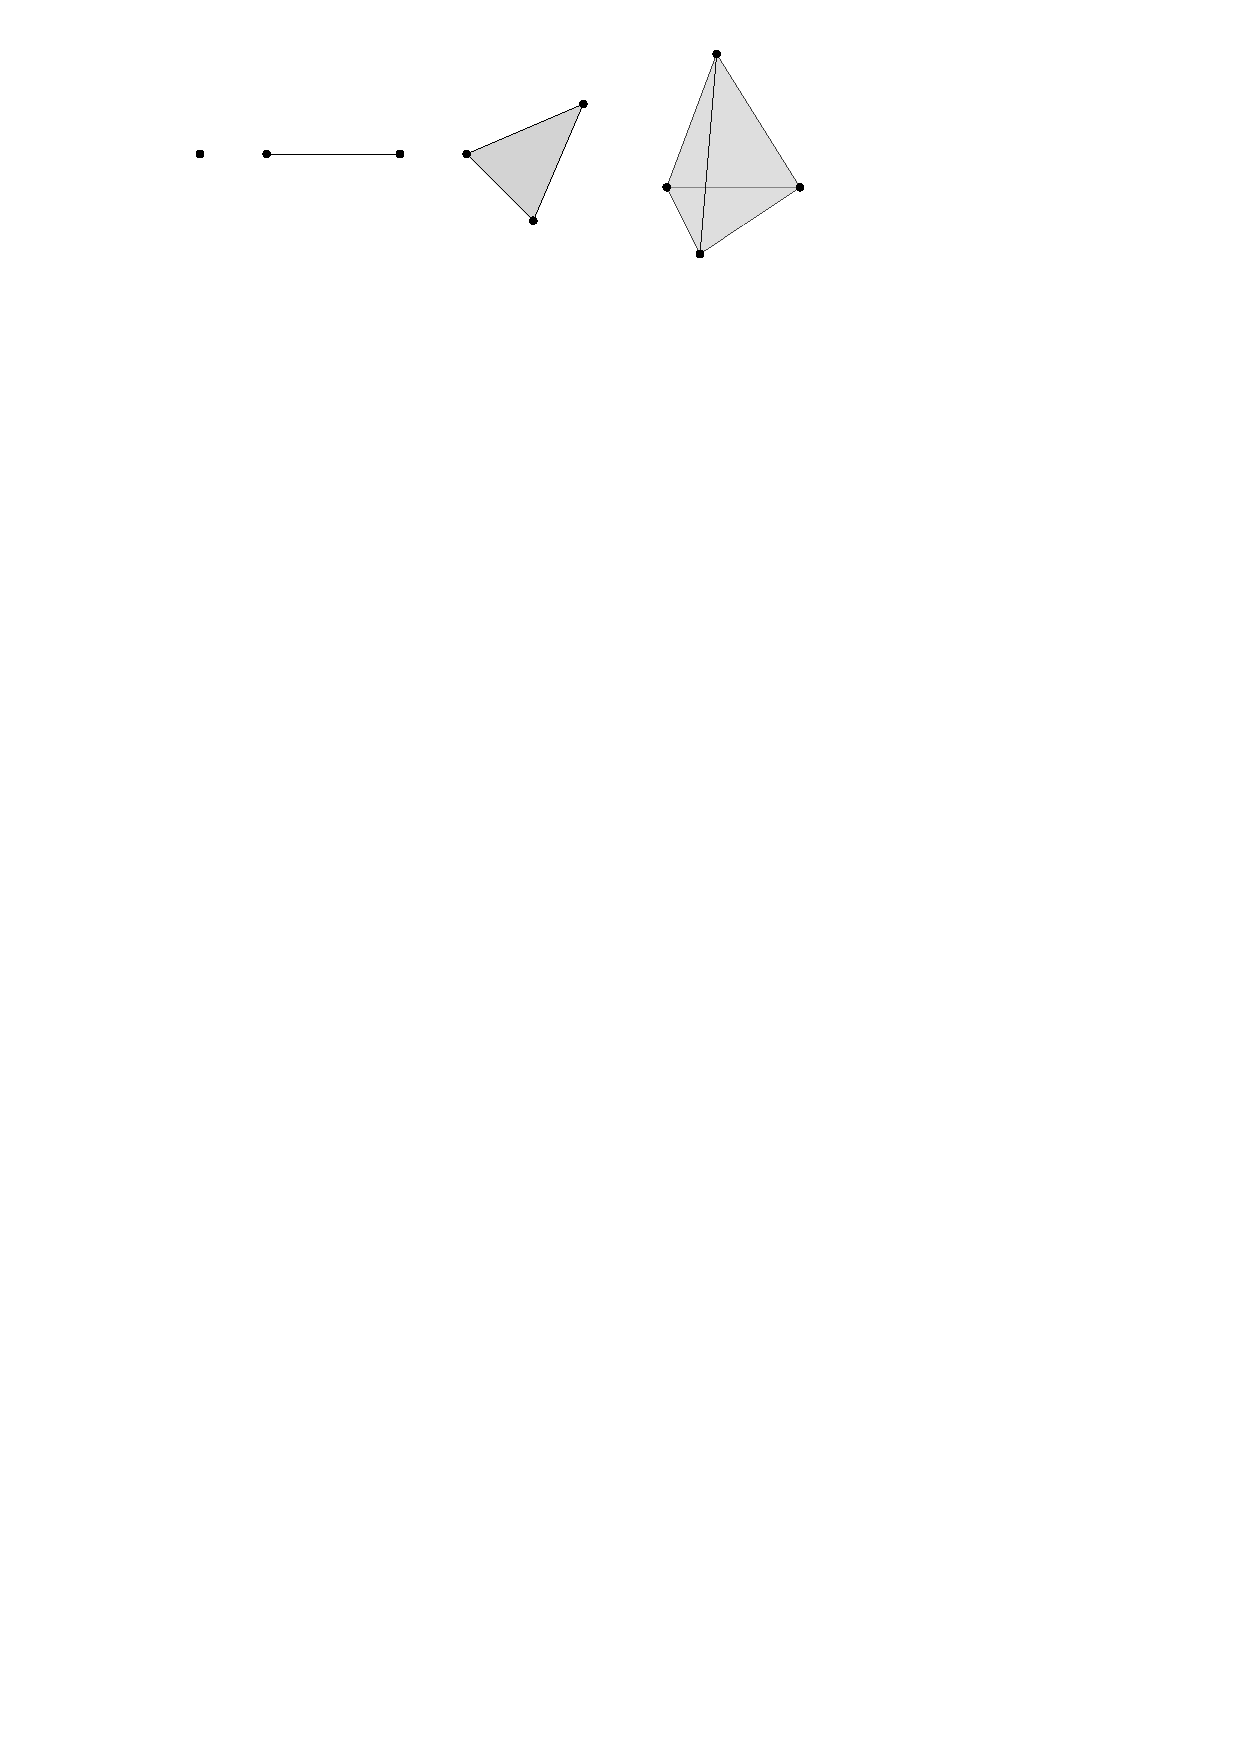
\includegraphics[width = 7cm]{figures/Simplices} 
\caption[Geometric simplices]{
Example of geometric simplices in dimension 0, 1, 2 and 3.} 
\label{fig:geomsimpl} 
\end{figure}
 

\begin{figure}[h] \centering 
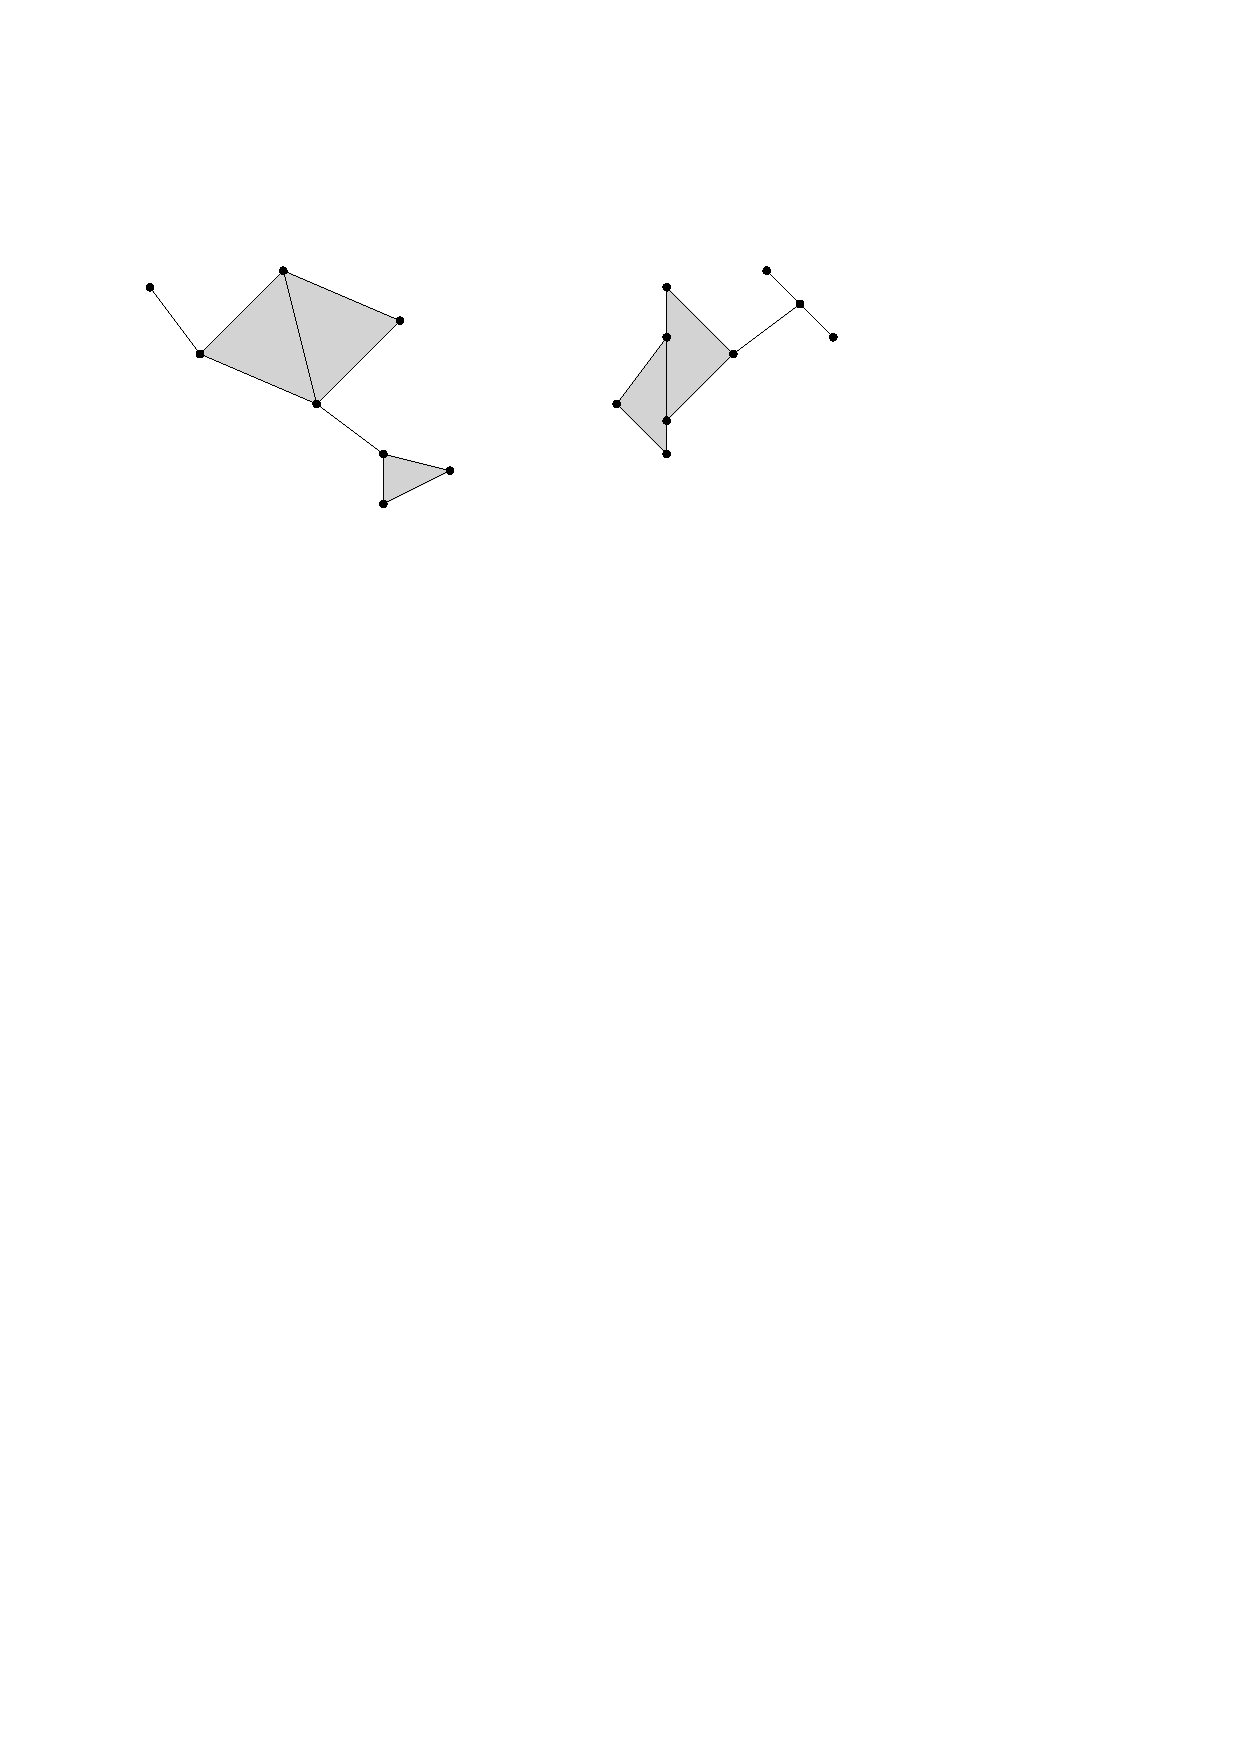
\includegraphics[width = 7cm]{figures/CounterExampleComplex} 
\caption[Geometric simplicial complex]{\label{fig:CEsimpl} The complex on the right hand side 
is not a geometric simplicial complex, because the intersection of the two 
triangles should be empty, as the triangles do not share any vertex, whereas it is not. 
The complex on the left hand side is a simplicial complex.} 
\end{figure}

\subsection{Simplicial Homology}
\label{sec:simplexHomo}

The definition of homology is based on {\em p-chains}, i.e. formal sums of simplices.

\begin{defin}
The set of $p$-chains of $K$, denoted by $C_{p}(K;\Z)$, is the free 
abelian group generated by the oriented $p$-simplices of $K$.
\end{defin} 

%Note that one can consider any ring $R$ instead of $\mathbb{Z}$, but it leads to heavier definitions. 
In practice, we often work with coefficients in a field, like $\Z_q=\Z/q\Z$ (if $q$ is a prime integer). 
%instead of $\mathbb{Z}$ as many operations are simplified in this field of coefficients.

%We now define the {\em boundary} of a simplex. and the {\em boundary operator} $\partial_{p}$.

\begin{defin} 
Let $\sigma$ be an oriented simplex of dimension $p$. 
The {\em boundary} of $\sigma$ is the $(p-1)$-chain given by the alternate 
sum of all of the oriented $(p-1)$-faces of $\sigma$. 
Formally, if $\sigma=[v_{0},\cdots,v_{p}]$, the boundary of $\sigma$ is: 
$$\sum_{i=0}^{p}(-1)^{i}[v_{0},\cdots,\hat{v}_{i},\cdots,v_{p}],$$ 
where $[v_{0},\cdots,\hat{v}_{i},\cdots,v_{p}]$ is the oriented $(p-1)$-face of $\sigma$, with missing $v_{i}$.
\end{defin}

By linearity, we extend the definition of the boundary to a $p$-chain of $K$. 
By convention, the boundary of a 0-chain is 0. The resulting 
{\em boundary operator} $\partial_{p}:C_{p}(K;\mathbb{Z})\rightarrow C_{p-1}(K;\mathbb{Z})$ 
sends a $p$-chain $c=\sum_{i}n_{i}\sigma_{i}$ to its boundary---see Figure~\ref{fig:bound}: 
$$\partial_{p}(c)=\sum_{i}n_{i}\partial_{p}(\sigma_{i}).$$ 

\begin{figure}[h]\centering 
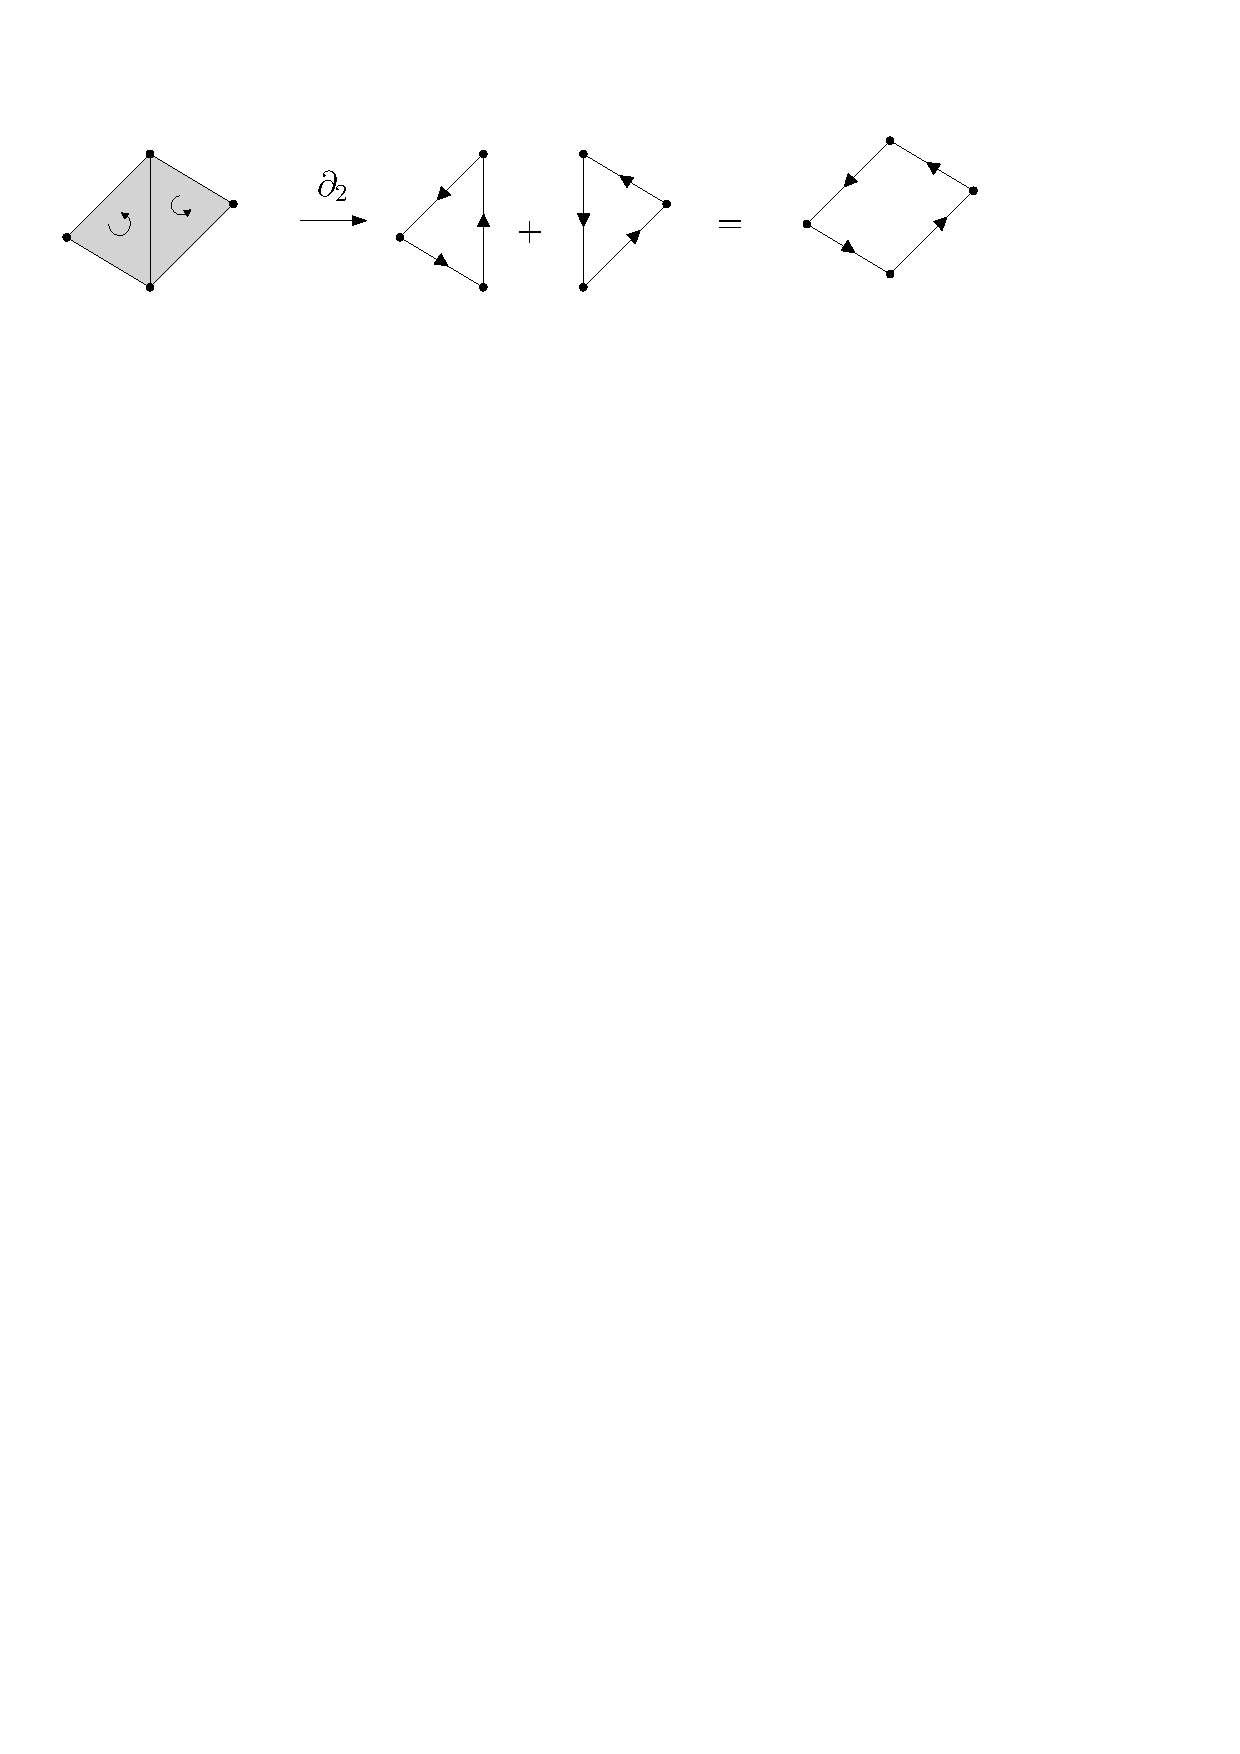
\includegraphics[width = 10cm]{figures/BoundaryOperator} 
\caption[Boundary operator]{\label{fig:bound} Action of the boundary operator on the sum of two oriented simplices. 
The middle edge cancels as it is counted twice with opposite orientations.} 
\end{figure}

\begin{defin} 
A {\em $p$-cycle} is a $p$-chain whose boundary is 0. 
The subgroup of all $p$-cycles is $\ker(\partial_{p})$.
\end{defin}

%An example of a 1-cycle in $\mathbb{Z}_{2}$ are 
%is shown in Figure~\ref{fig:cycles}. 
%In this field of coefficients, orientation does not matter, as $+$ and $-$ are the same operations. 
%Thus, the sum used to compute boundaries is no longer alternate, and simplices disappear when counted twice.

%See Figure~\ref{fig:cycles}. 

\begin{figure}[h] \centering
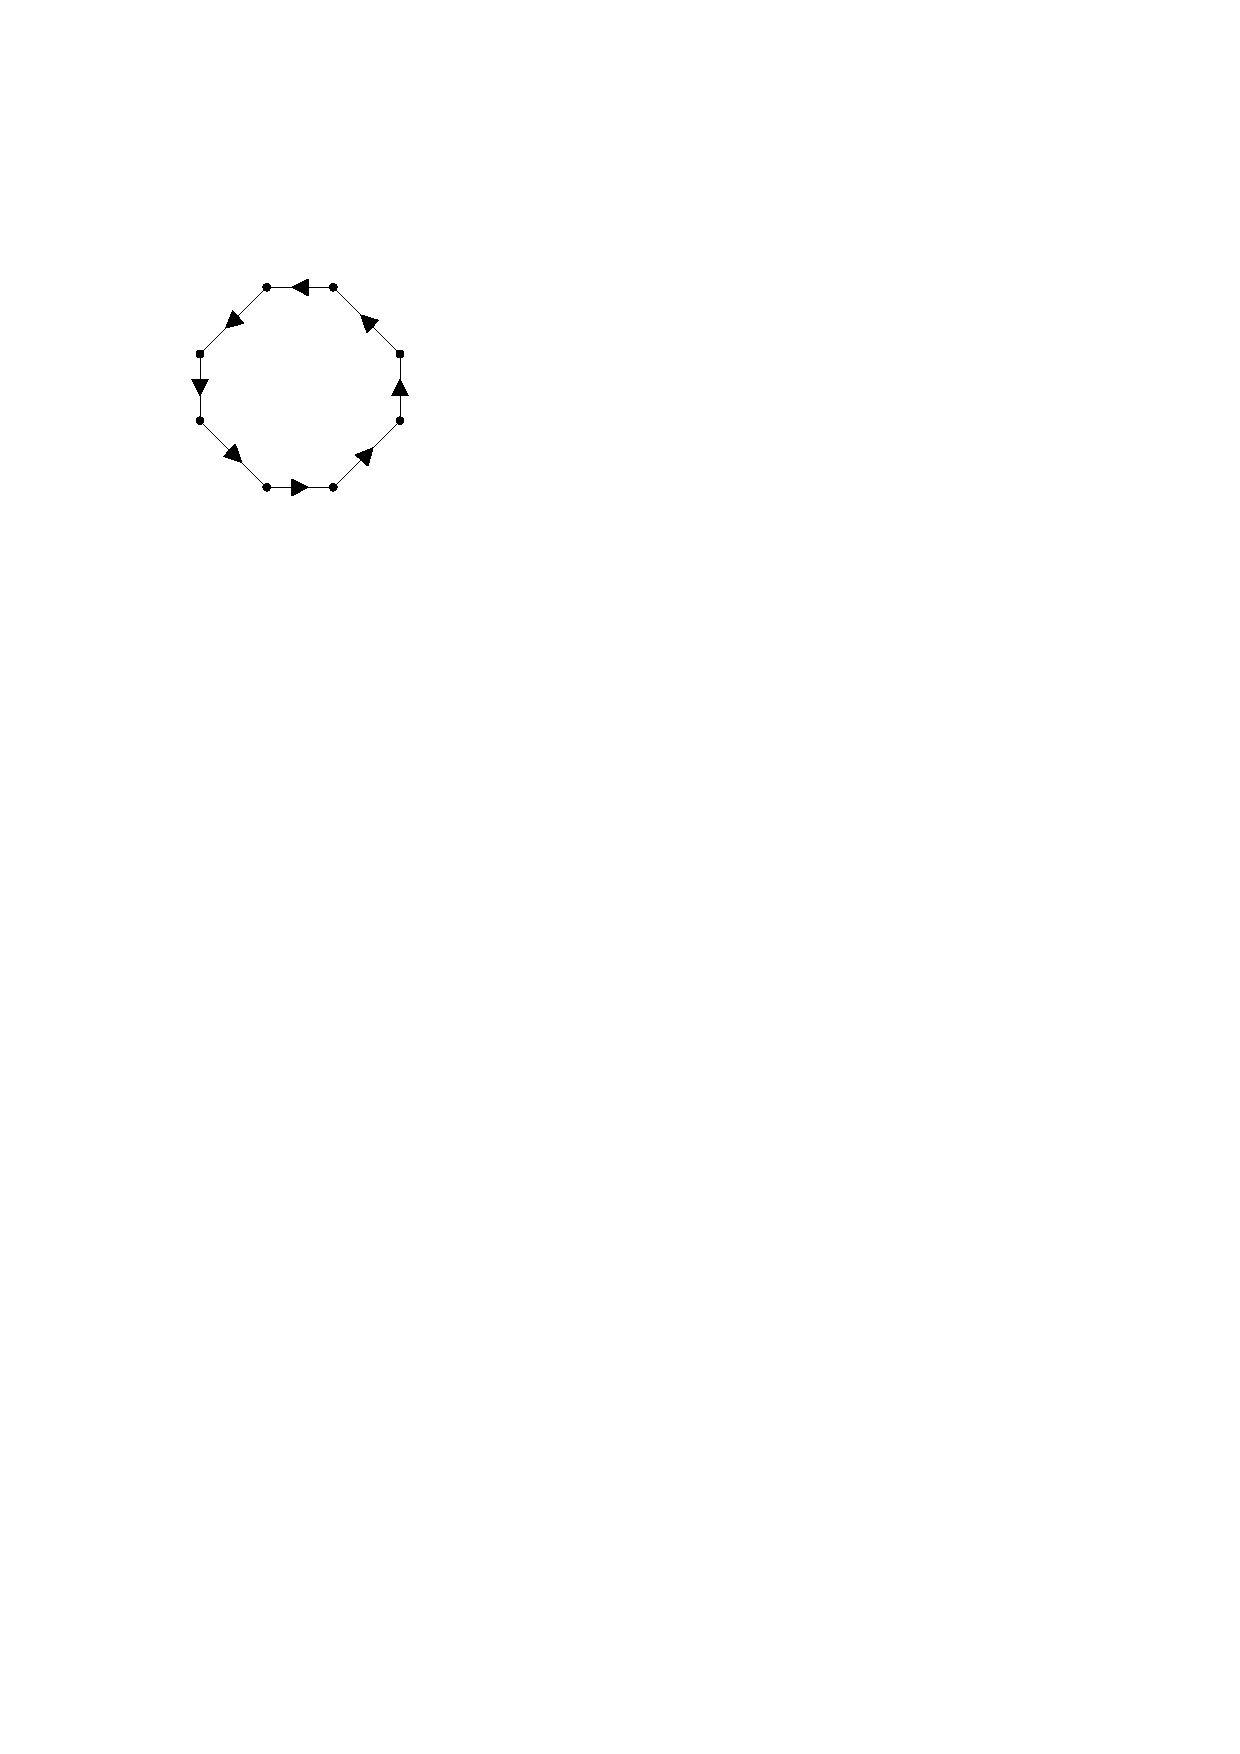
\includegraphics[width = 2cm]{figures/Cycles} 
\caption[Cycles]{\label{fig:cycles} Example of an oriented 1-cycle.} 
\end{figure}

Let us state the main property of the boundary operator:

\begin{prop} 
$\forall p\in \N^*,\ \partial_{p-1}\circ\partial_{p} = 0.$
\end{prop}

%\begin{proof} 
%Let $\sigma$ be a $p$-simplex. 
%If $\sigma=[v_{0}, \cdots, v_{p}]$, 
%then $\partial_{p}(\sigma)=\sum_{j=0}^{p}(-1)^{j}[v_{0}, \cdots,\hat{v}_{j}, \cdots,v_{p}]$ and: 
%\begin{align*}
%\partial_{p-1}\circ\partial_{p}(\sigma)& =\sum_{j}(-1)^{j}\partial_{p-1}([v_{0}, \cdots, \hat{v}_{j}, \cdots, v_{p}]) \nonumber\\
%& =\sum_{l>j}(-1)^{j}(-1)^{l-1}[v_{0},\cdots,\hat{v}_{j},\cdots,\hat{v}_{l},\cdots,v_{p}]\nonumber \\
%&\ \ \ \ \ \ \ \ \ +\sum_{l<j}(-1)^{j}(-1)^{l}[v_{0},\cdots,\hat{v}_{l},\cdots,\hat{v}_{j},\cdots,v_{p}]\nonumber\\
%&=0 \nonumber
%\end{align*}
%\end{proof}

Hence, we can extend this result to $p$-chains by linearity: if $c=\sum_{i}n_{i}\sigma_{i}$ then $\partial_{p-1}\circ\partial_{p}(c)=0$. 
This property allows to define a {\em chain complex}.

\begin{defin}
A {\em chain complex} $\mathcal C$ is a family of abelian groups $C_p$, $p\in\N^*$, together with homomorphisms 
$\phi_p:C_p\rightarrow C_{p-1}$ such that $\phi_{p-1}\circ\phi_p=0$.
%$$\cdots \overset{\partial_{p+1}}{\longrightarrow} C_p\overset{\partial_{p}}{\longrightarrow}C_{p-1}\overset{\partial_{p-1}}{\longrightarrow}\cdots$$
\end{defin}

In particular, the family of chain groups of a simplicial complex $K$ together with the boundary operators is a chain complex. 
In Sections~\ref{sec:singHomo} and~\ref{sec:relHomo}, we build other examples of chain complexes.
Since $\im(\phi_{p})\subseteq \ker(\phi_{p-1})$,
we can define the \textit{$p$th-homology group} of a chain complex as the quotient of those spaces.

\begin{defin}
The \textit{pth-homology group} of a chain complex $\mathcal C$ is: 
$$H_p(\mathcal C)={\rm ker}(\phi_{p})/\im(\phi_{p+1}).$$ 
\end{defin} 

In particular, the {\em simplicial pth-homology group} of a simplicial complex $K$ is: 
$$H_{p}(K;\mathbb{Z})={\rm ker}(\partial_{p})/\im(\partial_{p+1}).$$ 
A $p$-cycle in $\im(\partial_{p+1})$ is said to be \textit{trivial} and two equivalent $p$-cycles modulo 
$\im(\partial_{p+1})$ are said to be \textit{homologous}. If $K$ is a finite simplicial complex, then
$C_{p}(K;\Z)$ is finitely generated (by the $p$-simplices of $K$), and so is $H_p(K;\Z)$.

\begin{thm}[Decomposition of finitely generated abelian groups.]
\label{th:decomp} 
Every finitely generated abelian group $G$ is isomorphic to a 
direct sum of the form: $\mathbb{Z}^{n}\oplus\mathbb{Z}_{q_{1}}\oplus\cdots\oplus\mathbb{Z}_{q_{m}}$, 
where $q_{1},\cdots, q_{m}$ are powers of prime numbers. The integer $n$ is called the \textit{rank} of $G$, 
and $\oplus_{i=1}^{m}\mathbb{Z}_{q_{i}}$ is called the \textit{torsion subgroup} of $G$.
\end{thm}

\begin{defin} Let $K$ be a finite simplicial complex.
The {\em pth-Betti number} $\beta_{p}(K;\Z)$ of $K$, $p\in\N$, is the rank of $H_{p}(K;\Z)$.
\end{defin}

%In practice, we often change a little bit the definition of the Betti numbers by counting also 
%the number $m$ of finite cyclic groups in the torsion subgroup.
 
%\paragraph*{Coefficients in $\Z_2$.}
%When working in $\mathbb{Z}_{2}$, $H_{p}(K,\mathbb{Z}_{2})$ is not only finitely generated but also finite. 
%Theorem~\ref{th:decomp} states that $H_{p}(K,\mathbb{Z}_{2})$ is isomorphic to a direct sum of copies of 
%$\mathbb{Z}_{2}$. Thus, the rank is 0, and the Betti numbers $\beta_{p}(K,\mathbb{Z}_{2})$ 
%are the numbers of terms in the direct sum of the torsion subgroup. In that case, $H_{p}(K,\mathbb{Z}_{2})$ 
%can also be seen as a $\mathbb{Z}_{2}$-vector space, whose dimension is $\beta_{p}(K,\mathbb{Z}_{2})$.

\paragraph*{Interpretation.}
If we work with coefficients in $\Z_2$, then
the Betti numbers $\beta_{0}(K,\mathbb{Z}_{2})$, $\beta_{1}(K,\mathbb{Z}_{2})$ and $\beta_{2}(K,\mathbb{Z}_{2})$ can be 
interpreted as respectively the number of connected components of $K$, the number of holes in $K$ and the number of cavities, 
or voids, in $K$. To convince oneself, let us look at the 0-dimensional case. A 0-chain is a set 
of vertices of a simplicial complex. We claim that each of these vertices corresponds to a specific 
connected component. Indeed, if we select an arbitrary vertex in every connected component then every 
vertex of a given connected component is homologous to the corresponding arbitrary vertex. The proof is immediate: if 
two vertices $v_{1}$ and $v_{2}$ are in the same connected component, there exists a path of edges, or a 1-chain, 
between them. If we compute the boundary of this path, we get the boundary of every edge in the path, which consists 
of two vertices. As the edges in the path are linked, all the vertices will be counted twice and thus will disappear
(since the field of coefficients is $\Z_2$), 
except for the vertices at the beginning and the end of the path, in other words $v_{1}$ and $v_{2}$, that are 
thus homologous. On the contrary, no such path exists if the vertices are not in the same connected component.

\paragraph*{Example on the annulus.} 
To make these notions clearer, let us look at a specific example, the annulus of Figure~\ref{fig:annu}. 
As we said, $\beta_{0}$ is fairly easy to compute, it is equal to 1 in the example. Let us 
now look at $\beta_{1}$. We recall that in $\mathbb{Z}_{2}$, we do not consider orientations or 
alternate sums. Clearly, $\{a_{0},a_{1}\}+\{a_{1},a_{2}\}+\{a_{2},a_{0}\}$ is a 1-cycle because: 
\begin{align*}
\partial_{1} &(\{a_{0},a_{1}\}+\{a_{1},a_{2}\}+\{a_{2},a_{0}\})\nonumber\\
&=\partial_{1}(\{a_{0},a_{1}\})+\partial_{1}(\{a_{1},a_{2}\})+\partial_{1}(\{a_{2},a_{0}\})\nonumber\\
&=\{a_{0}\}+\{a_{1}\}+\{a_{1}\}+\{a_{2}\}+\{a_{2}\}+\{a_{0}\}=0\nonumber 
\end{align*} 
This cycle is also non trivial. Every other 1-cycle is homologous, for instance let us 
consider $\{a_{0},a_{1}\}+\{a_{1},a_{3}\}+\{a_{3},a_{2}\}+\{a_{2},a_{0}\}$, which is also non trivial. 
Then their sum is $\{a_{1},a_{3}\}+\{a_{3},a_{2}\}+\{a_{2},a_{1}\}$, which is trivial 
(it is the boundary of $\{a_{1},a_{2},a_{3}\}$). Thus $\beta_{1}=1$. 

\begin{figure}[h] \centering 
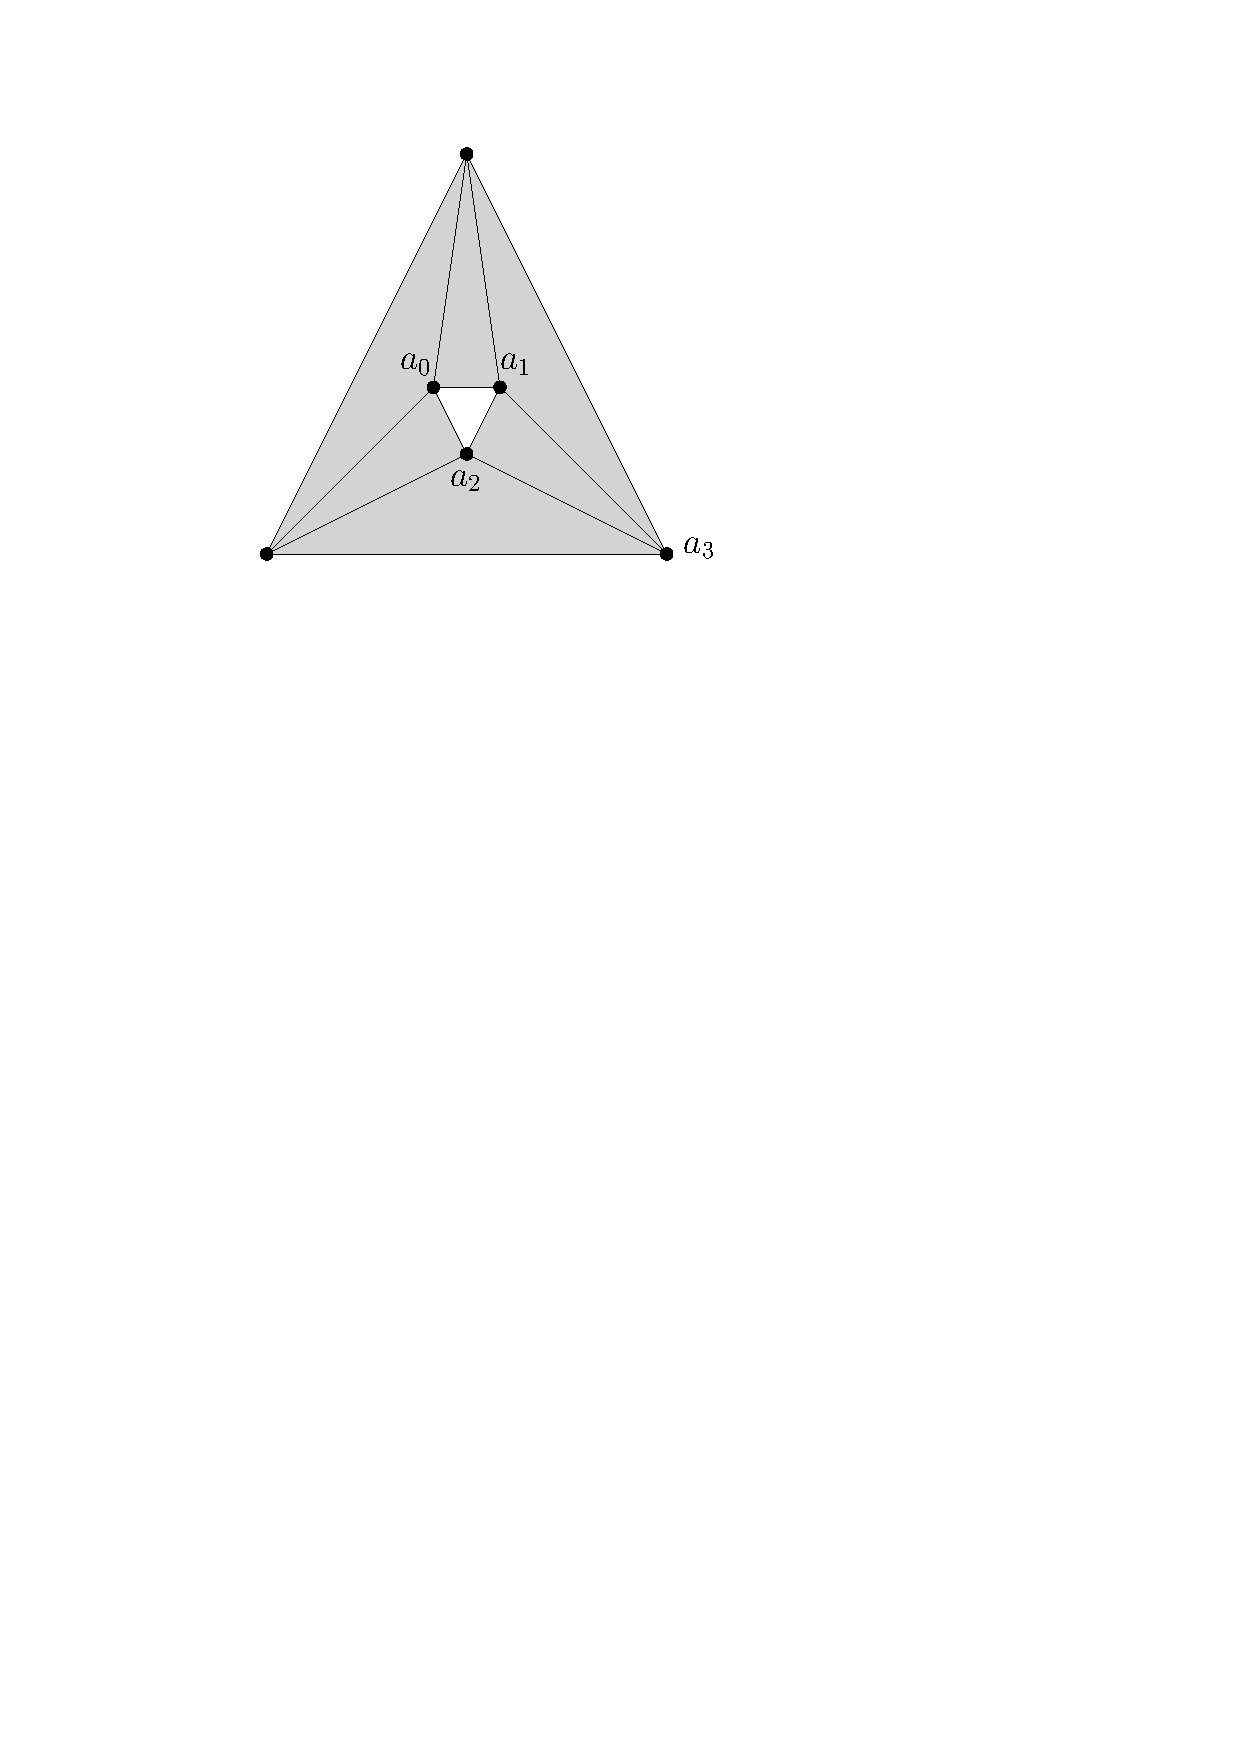
\includegraphics[width = 4cm]{figures/Annulus} 
\caption[Homology of annulus]{\label{fig:annu}
Example of simplicial complex representing an annulus. 
The Betti numbers are $\beta_{0}=\beta_{1}=1$.}
\end{figure}

\paragraph*{Morphisms between homology groups.}
Given several chain complexes, morphisms between their corresponding
homology groups can be built from {\em chain maps}.

\begin{defin}
Let 
$\mathcal C = \cdots \overset{\phi_{p+1}}{\longrightarrow} C_p\overset{\phi_{p}}{\longrightarrow}C_{p-1}\overset{\phi_{p-1}}{\longrightarrow}\cdots$ 
and $\mathcal C'=\cdots \overset{\phi'_{p+1}}{\longrightarrow} C'_p\overset{\phi'_{p}}{\longrightarrow}C'_{p-1}\overset{\phi'_{p-1}}{\longrightarrow}\cdots$
be chain complexes. A family of homomorphisms $f=\{f_p:C_p\rightarrow C'_p\}_{p\in\N}$ is a {\em chain map} if 
%\begin{equation}\label{eq:chaincomplex}
$$\phi'_p\circ f_p=f_{p-1}\circ \phi_p,$$
%\end{equation}
for any $p\in\N^*$. 
\end{defin}

\begin{prop}
A chain map $f:\mathcal C\rightarrow \mathcal C'$ induces a homomorphism $f_*:H_*(\mathcal C)\rightarrow H_*(\mathcal C')$.
Moreover, {\rm (i)} the identity map ${\rm id}$ of $\mathcal C$ is a chain map, and ${\rm id}_*$ is the identity map of $H_*(\mathcal C)$,
and {\rm (ii)} if $f:\mathcal C\rightarrow \mathcal C'$ and $g:\mathcal C'\rightarrow \mathcal C''$ are chain maps, then 
$g\circ f:\mathcal C\rightarrow \mathcal C''$ is a chain map and $(g\circ f)_*=g_*\circ f_*$. 
\end{prop}

%\begin{proof}
%It follows from~(\ref{eq:chaincomplex}) that $f_p({\rm ker}(\phi_p))\subseteq {\rm ker}(\phi'_p)$ 
%and $f_p({\rm im}(\phi_{p+1}))\subseteq {\rm im}(\phi'_{p+1})$. 
%Indeed, let $c\in C_p$ such that $\phi_p(c)=0$. 
%Then, $\phi'_p(f_p(c))=f_{p-1}(\phi_p(c))=f_{p-1}(0)=0$ since $f_p$ is a homomorphism. 
%Moreover, assume now that there is $d\in C_{p+1}$ such that $c=\phi_{p+1}(d)$.
%Then, $f_p(c)=f_p(\phi_{p+1}(d))=\phi'_{p+1}(f_{p+1}(d))\in{\rm im}(\phi'_{p+1})$. 
%Hence, $f_p$ induces a morphism $H_p(\mathcal C)\rightarrow H_p(\mathcal C')$.
%Items~{\rm (i)} and~{\rm (ii)} are straightforward.
%\end{proof}

\paragraph*{Morphisms between simplicial homology groups.} Chain maps between simplicial homology groups arise from {\em simplicial maps}
between simplicial complexes.

\begin{defin}
Let $K,L$ be two abstract simplicial complexes.
A map $f:V(K)\rightarrow V(L)$ is a {\em simplicial map} if
$\{v_0,\cdots,v_p\}\in K\Rightarrow \{f(v_0),\cdots,f(v_p)\}\in L$.
\end{defin}

%The domain of any simplicial map can be extended to the whole set of oriented simplices %of an abstract simplicial complex 
%with $f(\sigma)=f([v_0,\cdots,v_p])=[f(v_0),\cdots,f(v_p)]$.

\begin{prop}
Let $K,L$ be two abstract simplicial complexes, and
$f:V(K)\rightarrow V(L)$ be a simplicial map.
Then, $f$ induces a chain map between the chain complexes $\{C_p(K;\Z),\partial_p\}_{p\in\N}$ and $\{C_p(L;\Z),\partial_p\}_{p\in\N}$.
%In particular, $f$ induces a morphism $f_*:H_*(K)\rightarrow H_*(L)$.
%Moreover, one has $({\rm id})_*={\rm id}_{H_*}$, and, given a third simplicial complex $M$ and a second simplicial map $g:V(L)\rightarrow V(M)$, 
%between $L$ and , 
%we have $(g\circ f)_*=g_*\circ f_*$.
\end{prop}

%\begin{proof}
%Let $f_p:C_p(K;\Z)\rightarrow C_p(L;\Z)$ be defined with $f_p(\sum_i n_i\sigma_i)=\sum_i n_i f(\sigma_i)$.
%Then, by linearity of $\partial_p$, we have $\partial_p\circ f_p(\sum_i n_i \sigma_i)=
%\partial_p(\sum_i n_i f(\sigma_i))=\sum_i n_i \partial_p\circ f(\sigma_i)$. Now, again by linearity of $\partial_p$,
%$f_{p-1}\circ\partial_p(\sum_i n_i \sigma_i)=f_{p-1}(\sum_i n_i \partial_p(\sigma_i))=\sum_i n_i f\circ\partial_p(\sigma_i)$.
%Hence, it only remains to show that $f$ commutes with $\partial_p$ on all $p$-simplices $\sigma_i$.

%Let $\sigma=[v_0,\cdots,v_p]$ be such a simplex. Then, 
%\begin{align*}
%& f\circ\partial_p(\sigma)=f(\sum_{j=0}^{p}(-1)^{j}[v_{0}, \cdots,\hat{v}_{j}, \cdots,v_{p}])=\sum_{j=0}^{p}(-1)^{j}f([v_{0}, \cdots,\hat{v}_{j}, \cdots,v_{p}])\\
%&=\sum_{j=0}^{p}(-1)^{j}[f(v_{0}), \cdots,\widehat{f(v_{j})}, \cdots,f(v_{p})])=\partial_p([f(v_0),\cdots,f(v_p)])=\partial_p\circ f(\sigma).
%\end{align*}
%\end{proof}



\subsection{Singular Homology}
\label{sec:singHomo}

Other chain complexes can be defined if the space under consideration is not a simplicial complex.
This can be done using the so-called {\em singular homology}. Intuitively, singular simplices are
images of usual simplices under continuous functions.
%The proofs in this Section follow 
%closely the ones of Section~\ref{sec:simplexHomo}, so we do not explicit all of them. 
We refer the interested reader to~\cite{Munkres93} for further details. 

\begin{defin}
Let $\Sigma_p=\{v_1,\cdots,v_{p+1}\}$ be the {\em oriented standard $p$-simplex}, i.e. the geometric simplex in $\R^{\infty}$
whose vertices are defined by $v_i=e_i$, where $e_i$ is the $i$th element of the standard basis %an the canonical orthonormal family 
of $\R^{\infty}$, %with $p+1$ elements, 
together with the orientation induced by the basis ordering. %of these $p+1$ elements.
Let $X$ be a topological space. An {\em oriented singular $p$-simplex} of $X$ is the image of $\Sigma_p$ under a 
continuous mapping $\sigma:\Sigma_p\rightarrow X$,
together with an orientation induced by the one of $\Sigma_p$.
We write $\sigma([v_1,\cdots,v_{p+1}])$ to denote such a simplex together with its orientation. 
%When we want to specify the orientation, we write $[\sigma]$
%instead of $\sigma$.  
\end{defin}

Note that $\sigma$ need not be injective. It may be the constant map for instance. We give an example of an
oriented singular 2-simplex in Figure~\ref{fig:ExampleSing}.

\begin{figure}\centering
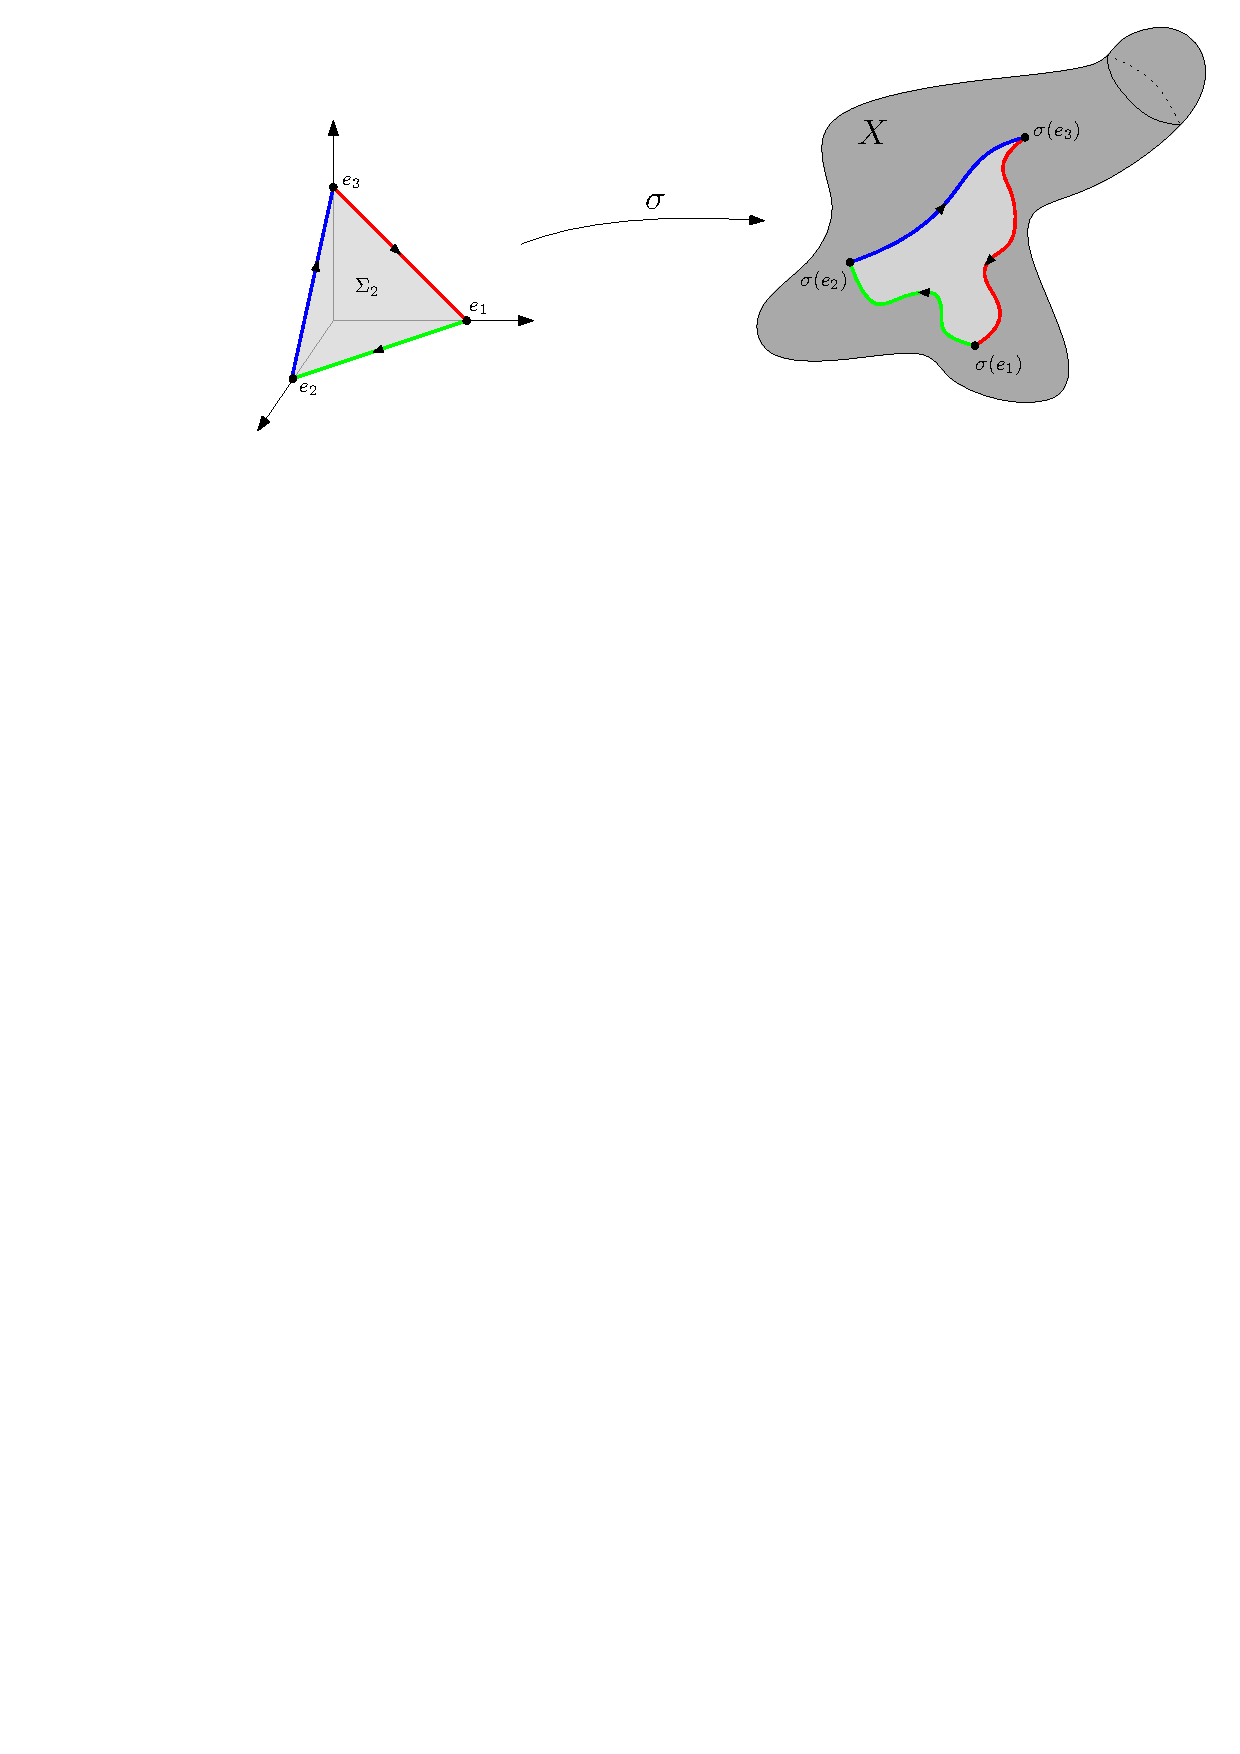
\includegraphics[width=13cm]{figures/ExampleSingularSimplex}
\caption[Singular simplex]{\label{fig:ExampleSing} Oriented singular 2-simplex $\sigma$ on a 3D surface $X$.}
\end{figure} 

\paragraph*{Singular homology groups.} All the definitions in the previous section extend almost directly.
The group of {\em singular $p$-chains} is defined as the free abelian group generated by the oriented singular
$p$-simplices of $X$. Note that this group may contain uncountably many generators.
The {\em (singular) boundary operator} $\partial^{\rm sing}_p$ is defined on a singular simplex as:
$$\partial^{\rm sing}_p(\sigma([v_1,\cdots,v_{p+1}]))=\sum_{i=1}^{p+1}(-1)^i \sigma_i([v_1,\cdots,\hat v_i,\cdots,v_{p+1}]),$$
where $\sigma_i$ is the restriction of $\sigma$ on the $(p-1)$-face of $\Sigma_p$ induced by the removal of $v_i$.
It is then extended by linearity to singular chains, and
%The chains that have null boundary are called {\em singular cycles}. 
we have again $\partial^{\rm sing}_p\circ\partial^{\rm sing}_{p+1}=0$, so we can define a chain complex with these boundary operators.
Hence, we define the {\em singular  $p$th-homology group} of $X$ as $H_p(X;\Z)=\ker(\partial^{\rm sing}_p)/\im(\partial^{\rm sing}_{p+1})$,
i.e. the group of those singular $p$-chains with null boundary (also called {\em singular $p$-cycles}) 
that are not images by $\partial_{p+1}$ of singular $(p+1)$-chains.  
%An interesting property of homology is to be invariant to homeomorphism.

\paragraph*{Singular and simplicial homologies.} Given an abstract simplicial complex $K$
and a geometric realization $|K|$ thereof, one may ask for the relationships between the
simplicial homology groups of $K$ and the singular homology groups of $|K|$.
It turns out that they are essentially the same:

\begin{prop}[\S 34 in Chapter 4 in~\cite{Munkres93}]\label{prop:SingSimpl}
Let $K$ be an abstract simplicial complex and let $|K|$ be a geometric realization of $K$.
Then, the singular homology groups of $|K|$ and the simplicial homology groups of $K$ are isomorphic.
\end{prop}

\paragraph*{Morphisms between singular homology groups.}
There is an easy way to build chain maps between the chain complexes induced by the singular chain groups of two spaces $X$ and $Y$.
%and their corresponding boundary operators.
%the singular homology groups of different topological spaces.
Indeed, given a function $f:X\rightarrow Y$, continuity is a sufficient requirement to build such a chain map.

\begin{prop}[Theorems 29.1 and 29.2 in~\cite{Munkres93}]\label{prop:inducedSingular}
Let $X,Y$ be topological spaces and $f:X\rightarrow Y$ be a continuous function. Then, $f$ induces a
chain map between the chain complexes $\{C_p(X;\Z),\partial_p\}_{p\in\N}$ and $\{C_p(Y;\Z),\partial_p\}_{p\in\N}$. 
%morphism $f_*:H_*(X)\rightarrow H_*(Y)$.
%Moreover, one has $({\rm id})_*={\rm id}_{H_*}$, and, given a third topological space $Z$ and a second continuous function $g:Y\rightarrow Z$, 
%we have $(g\circ f)_*=g_*\circ f_*$.
\end{prop}

\paragraph*{Invariance to homotopy equivalence.} One of the key properties of homology groups
is their invariance to continuous deformations of spaces. To formalize this, we use the notion of {\em homotopy equivalence}
between topological spaces.

\begin{defin}\label{def:homotopy}
Let $X,Y$ be topological spaces, and let $f,f':X\rightarrow Y$ be continuous functions. The functions $f$ and $f'$
are said to be {\em homotopic} if there exists a continuous function $F:X\times [0,1]\rightarrow Y$ such that $F(\cdot,0)=f$ and $F(\cdot,1)=f'$.
The spaces $X$ and $Y$ are said to have {\em the same homotopy type}, or to be {\em homotopy equivalent}, 
if there exist $f:X\rightarrow Y$ and $g:Y\rightarrow X$ such that
$f\circ g$ is homotopic to ${\rm id}_Y$ and $g\circ f$ is homotopic to ${\rm id}_X$.
\end{defin}

Note that if $X$ and $Y$ are homeomorphic, i.e. there exists a continuous bijection $f:X\rightarrow Y$ such that the inverse $f^{-1}$ is also
continuous, then they have the same homotopy type (it suffices to take $g=f^{-1}$ in Definition~\ref{def:homotopy}).
Proposition~\ref{prop:inducedSingular} allows to show the following proposition, which states that homology is
invariant under homotopy equivalences---and thus also under homeomorphisms.

\begin{prop}
Let $X,Y$ be homotopy equivalent topological spaces. Then $H_*(X;\Z)\simeq H_*(Y;\Z)$.
\end{prop}

%\begin{proof}
%Let $f:X\rightarrow Y$ and $g:Y\rightarrow X$ be continuous functions such that $f\circ g$ is homotopic to ${\rm id}_Y$
%and $g\circ f$ is homotopic to ${\rm id}_X$. Then, $({\rm id}_Y)_*={\rm id}_{H_*(Y;\Z)}=(f\circ g)_*=f_*\circ g_*$.
%Since ${\rm id}_{H_*(Y;\Z)}$ is an isomorphism, it follows that $g_*$ is injective. Similarly,
%$g_*\circ f_*={\rm id}_{H_*(X;\Z)}$ is also an isomorphism, and $g_*$ is also surjective. Hence, $g_*:H_*(Y;\Z)\rightarrow H_*(X;\Z)$
%is an isomorphism of homology groups, which we denote by $H_*(X;\Z)\simeq H_*(Y;\Z)$.  
%\end{proof}

In particular, if a topological space $X$ is triangulable, then there is an abstract simplicial complex $K$ such that
$X$ and $|K|$ are homeomorphic. Thus, the singular homology groups of $X$ are isomorphic to the ones 
of $|K|$, which in turn are isomorphic to the simplicial homology groups of $K$. 

\subsection{Relative Homology}\label{sec:relHomo}

Relative homology groups are computed with pairs of topological spaces.
As for singular homology, it is a simple extension of simplicial homology.

\begin{defin}
Let $Y\subseteq X$ be topological spaces. Let $C_p(X;\Z)$ and $C_p(Y;\Z)$ be the groups of
$p$-chains of $X$ and $Y$ respectively. Then, the group of {\em relative $p$-chains} is the
quotient group: $$C_p(X,Y;\Z)=C_p(X;\Z)/C_p(Y;\Z).$$
\end{defin} 

\paragraph*{Relative homology groups.} The usual boundary operator commutes with the inclusion:
letting $\iota_p:C_p(Y;\Z)\hookrightarrow C_p(X;\Z)$ denote the canonical inclusion, we have
$\partial_p\circ\iota_p = \iota_{p-1}\circ\partial_p$.
Hence, $\partial_p$ induces the
{\em (relative) boundary operator} $\partial^{\rm rel}_p:C_p(X,Y;\Z)\rightarrow C_{p-1}(X,Y;\Z)$, 
%is well defined (it suffices to compose the usual boundary operator, with the map induced by the quotient of the groups of $p$-chains) 
which satisfies $\partial^{\rm rel}_{p}\circ\partial^{\rm rel}_{p+1}=0$. Once again, this allows to define
a chain complex, which in turn induces the so-called {\em relative $p$th-homology group} with $H_p(X,Y;\Z)=\ker(\partial^{\rm rel}_p)/\im(\partial^{\rm rel}_{p+1})$.  Note
that these definitions hold also for abstract simplicial complexes.

\paragraph*{Example.} It is easy to build examples where homology and relative homology differ.
For instance, any $p$-chain included in $Y$ is trivial in $C_p(X,Y;\Z)$. It may also happen
that $p$-chains of nonzero boundary with the usual boundary operator become $p$-cycles in relative homology.
See Figure~\ref{fig:RelHom} for instance.


\begin{figure}\centering
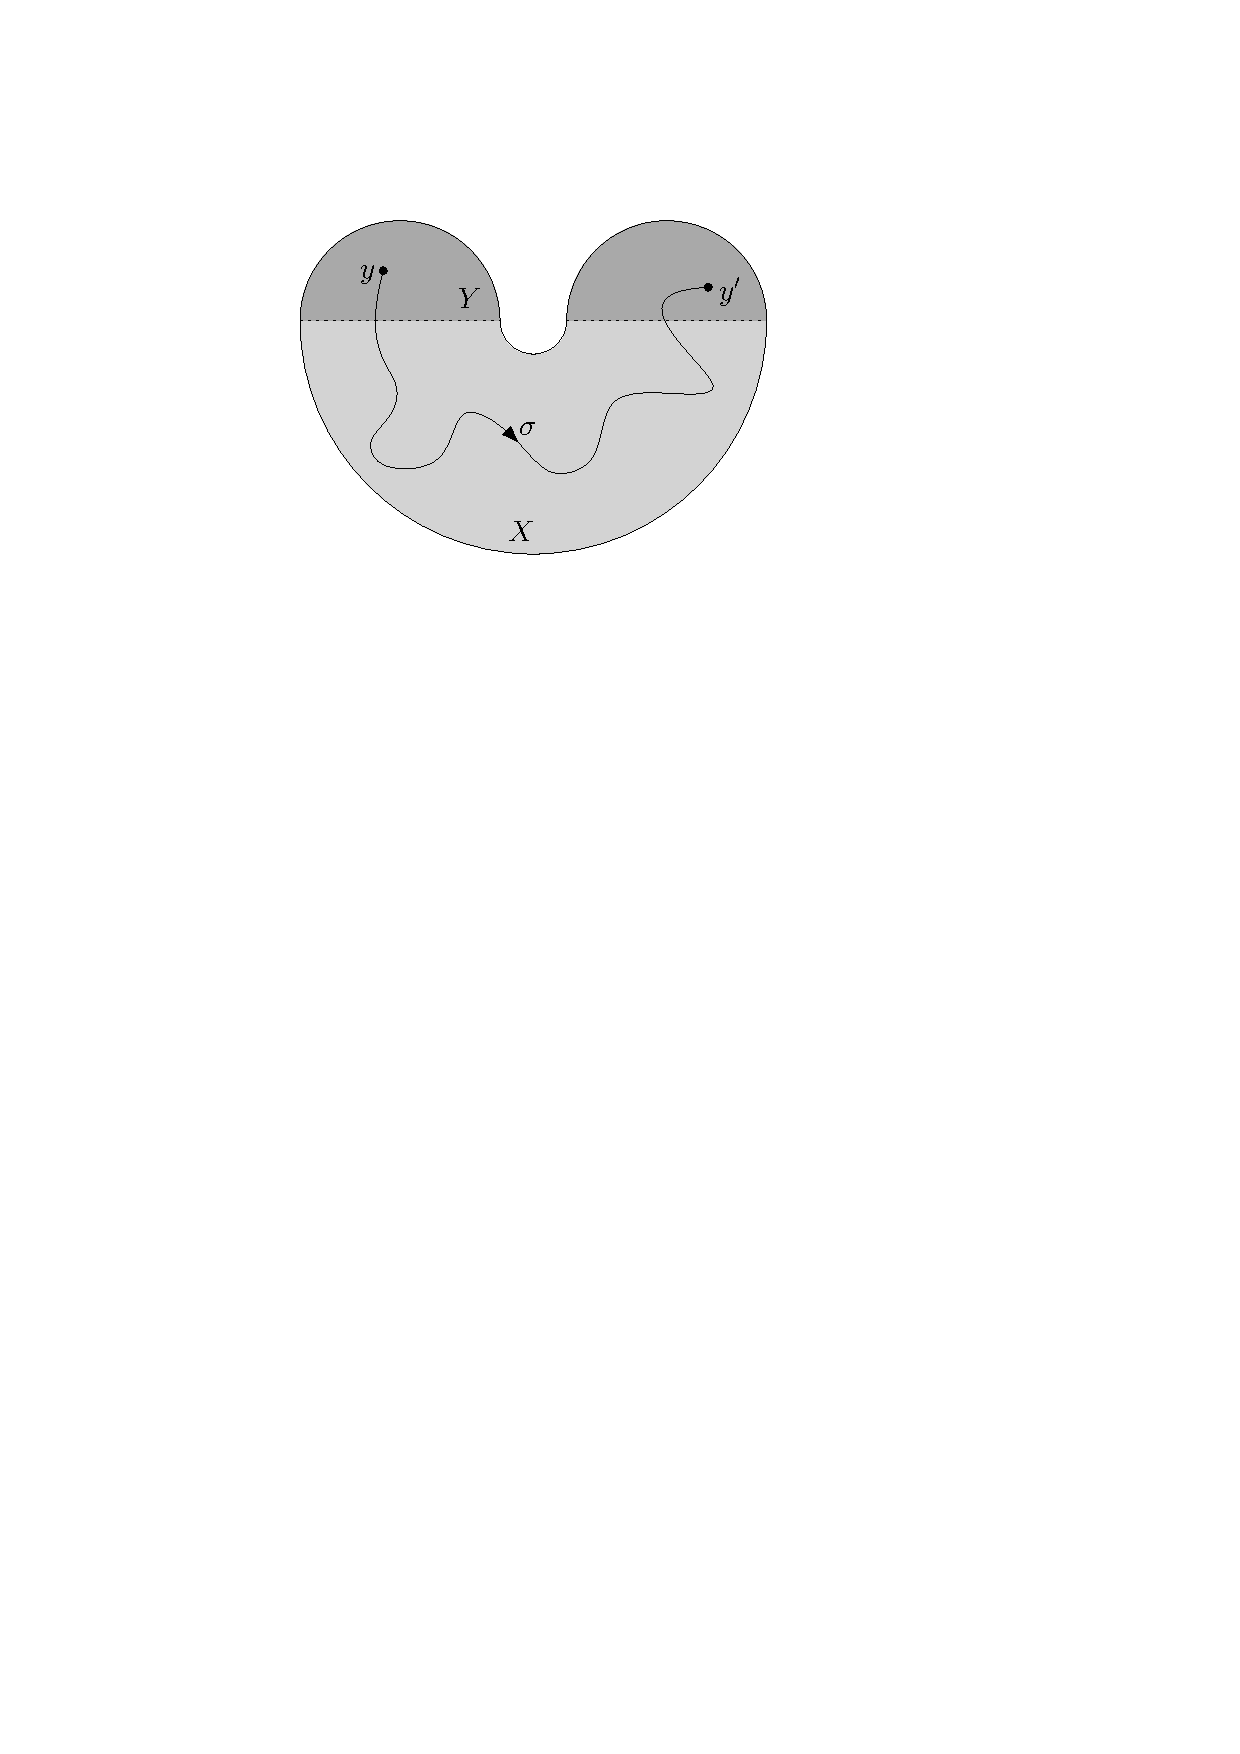
\includegraphics[width=5cm]{figures/CounterExampleRelHom}
\caption[Relative cycle]{\label{fig:RelHom} In this example, we study the pair of spaces $Y\subseteq X$. The oriented singular 1-simplex $\sigma=[y,y']$
has boundary $[y']-[y]\in Y$. Hence, $\partial_1(\sigma)\neq 0$ while $\partial^{\rm rel}_1(\sigma)=0$:
$\sigma$ is a cycle in relative homology but not in usual homology.}
\end{figure}















\section{Persistence Theory}
\label{sec:persistence}

We now describe persistent homology for topological spaces.
However, we recall from Proposition~\ref{prop:SingSimpl} that all definitions
hold for simplicial complexes as well.
%We define {\em filtrations} and {\em modules} in Sections~\ref{sec:filtrations} and~\ref{sec:modules} respectively,
%from which we can define the {\em persistence diagrams} in Section~\ref{sec:defPD}. Finally, their {\em stability}
%is derived in Section~\ref{sec:stabilityPD}.

\subsection{Filtrations}\label{sec:filtrations}

%A lot of the following notions were studied in~\cite{Chazal16a}. 
%Let us start with a basic yet important object: a {\em filtration}.
Intuitively, the aim of persistence is to study the evolution of the homology groups through a %so-called 
{\em filtration}. 

\begin{defin} \label{def:filt}
A {\em filtration} 
%of a topological space $X$ 
is an $\R$-indexed family of topological spaces  $\{X_{\alpha}\}_{\alpha\in\R}$ 
that are nested with respect to  inclusion, %which is 
%subsets of $X$ 
%indexed by the real line. 
%It is a family
that is $s\leq t\Rightarrow X_s\subseteq X_t$.
%$\emptyset =X_{0}\subseteq X_{1}\subseteq\ \cdots\ \subseteq X_{n}=X$.
\end{defin} 

Note that, when the $X_{i}$ are simplicial complexes, %must be a subcomplex of $K$, 
Definition~\ref{def:filt} means that a simplex $\sigma_{i}\in X_i$ cannot appear in the filtration before its faces.


%A standard way to build filtrations uses the {\em sublevel sets of functions}.

\begin{defin} 
Let $f:X\rightarrow\mathbb{R}$ be a continuous function defined on a topological space $X$. 
The filtration $\{F_{\alpha}\}_{\alpha\in\mathbb{R}}$ {\em induced by} $f$ is the filtration 
composed of the sublevel sets of $f$: %$\sigma\in K_{\alpha}\Leftrightarrow f(\sigma)\leq\alpha$, 
%in other words 
$F_{\alpha}=f^{-1}((-\infty,\alpha])$.
\end{defin}

One cannot choose just any function to build a filtration. For instance, when the spaces are simplicial complexes, 
the value of $f$ on a  simplex $\sigma$ must be superior to its values on all the faces of $\sigma$, so that 
the faces of $\sigma$ are included in the filtration before $\sigma$ itself. We must have: 
$$\forall\sigma\in X_i,\ \tau\text{ is a face of }\sigma\ \Rightarrow\ f(\tau)\leq f(\sigma).$$ 
A classical way to accomplish this is to define the values of $f$ on $V(K)$ and to define $f$ on simplices of dimension $p>0$
in the following way: $f(\{v_0,\cdots,v_p\})=\max\{f(v_0),\cdots, f(v_p)\}$. 
This is also known as the \textit{lower-star filtration of f}. See Figure~\ref{fig:lowstar}, where a function 
is defined on the 8 vertices of a simplicial complex $K$. The order of appearance of 
the simplices depends on the values of $f$ at these vertices. 

\begin{figure}[h] \centering
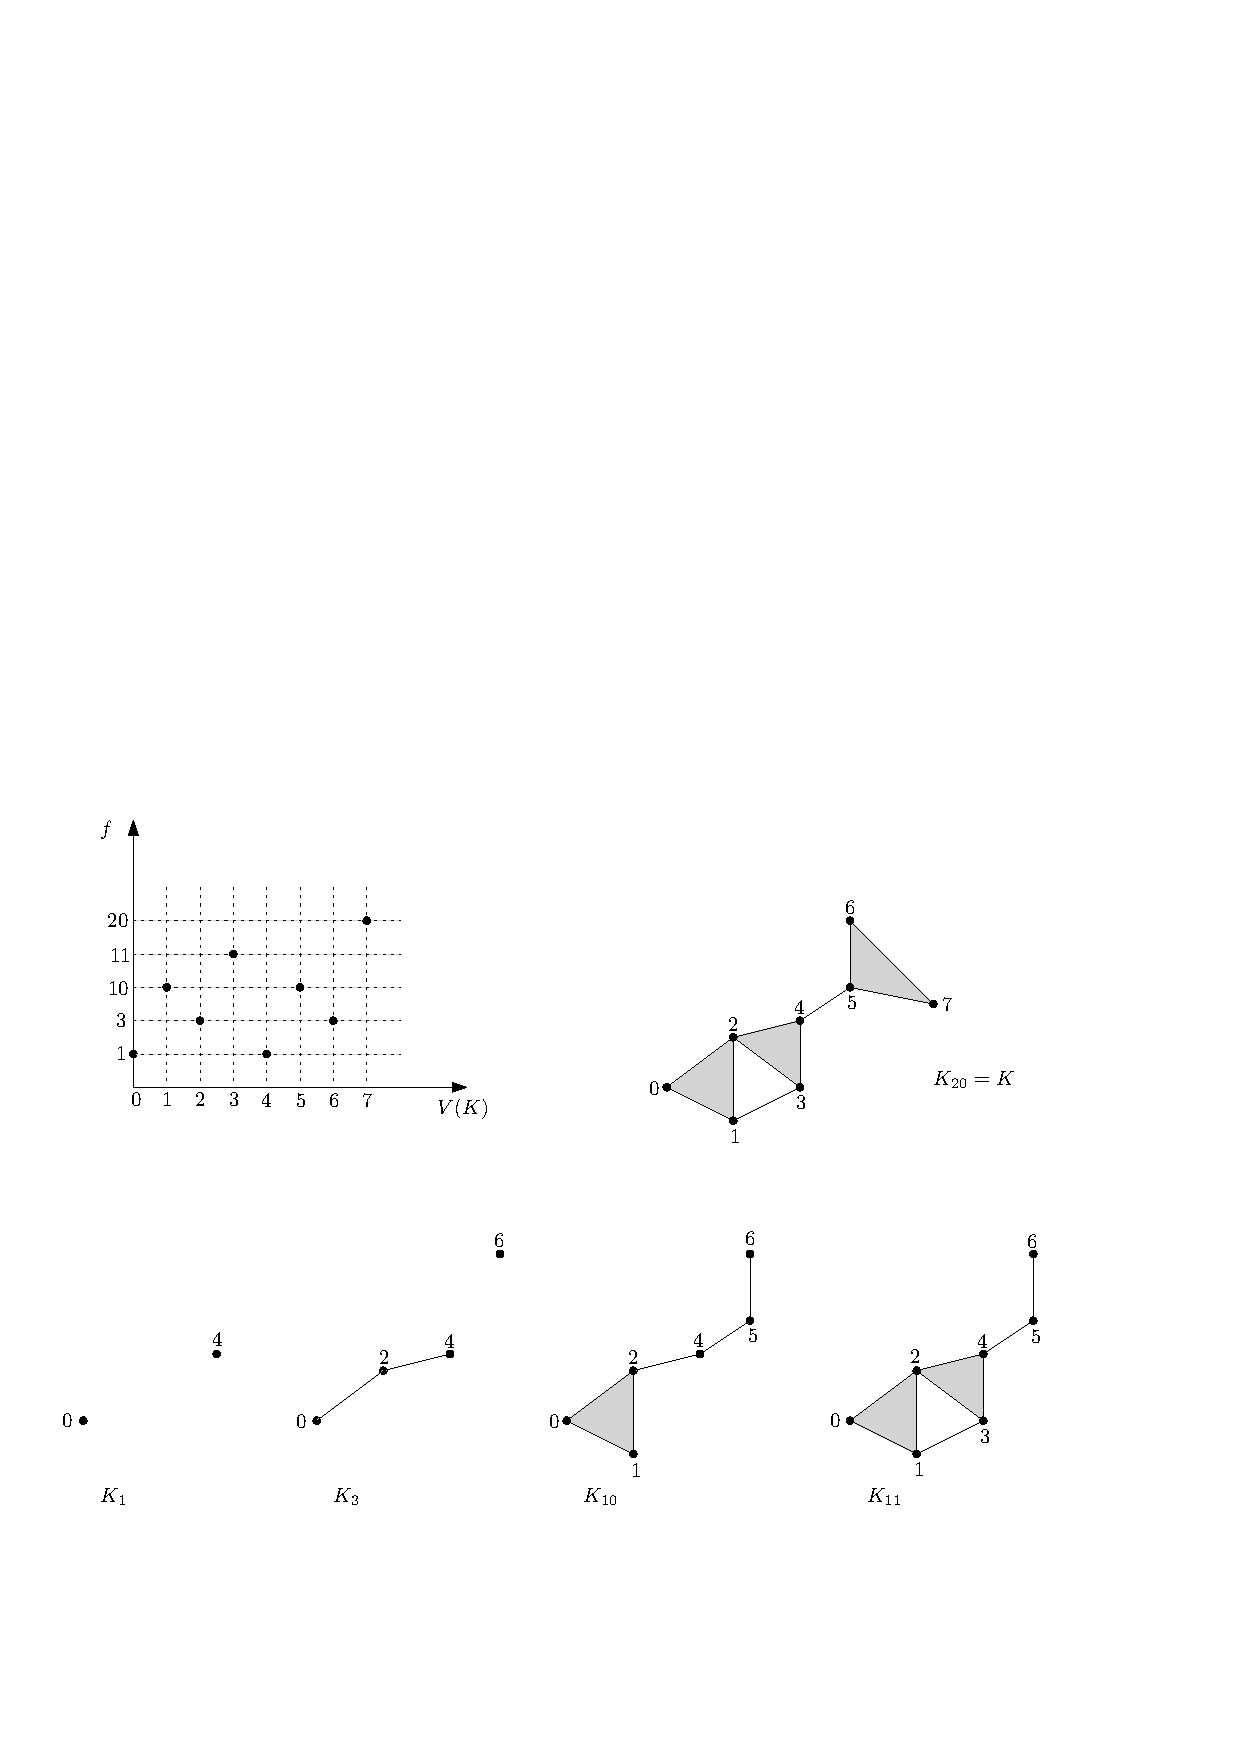
\includegraphics[width = 13cm]{figures/LowStar} \caption[Lower-star filtration]{\label{fig:lowstar}
Example of lower star filtration of a function $f$} 
\end{figure}

%\paragraph*{Rips filtration.}
%The aim of persistence is to study the evolution of the homology groups through a filtration. 
%Before formalizing this, 
%We now define a very common filtration of simplicial complexes built on a set of points in $\mathbb{R}^{D}$: 
%the \textit{\v{C}ech filtration} and 
%the \textit{Rips filtration}. 
%We will use it later in Chapter~\ref{chap:MapperStatistic}.

%\begin{defin} 
%Let $P$ be a finite point cloud in $\mathbb{R}^{D}$: $P=\{p_{0},\cdots,p_{n}\}$. 
%Let $B(x,r)$ be the open ball centered at $x\in\mathbb{R}^{D}$ with radius $r>0$. 
%The \textit{\v{C}ech filtration $\{C_{\alpha}\}_{\alpha\in\mathbb{R}_{+}}$} of $P$ is defined by: 
%$$\sigma=\{p_{i_{0}},\cdots, p_{i_{k}}\}\in C_{\alpha}\ \Leftrightarrow\ \bigcap_{j=0}^{k}B(p_{i_{j}},\alpha)\neq \emptyset.$$ 
%Note that this is a filtration of the $n$-dimensional abstract simplex $\{p_{0},\cdots,p_{n}\}$.
%\end{defin}

 

%\begin{defin}
%The {\em Rips filtration} $\{\Rips_{\delta}\}_{\delta\in\mathbb{R}_{+}}$ of a point cloud $P\subset \R^D$ is a filtration of abstract simplicial complexes defined by: 
%$$\sigma=\{p_{i_{0}},\cdots, p_{i_{k}}\}\in \Rips_{\delta}\ \Leftrightarrow\ {\rm diam}(\{p_{i_{0}},\cdots,p_{i_{k}}\})\leq\delta,$$
%where the {\rm diameter} of a set of points in $\mathbb{R}^{D}$ is the maximal Euclidean distance between any pair of points. %in the set.
%\end{defin}

\subsection{Persistence Modules}\label{sec:modules}
%Persistence theory aims at studying the structure of \textit{persistence modules}. These objects can be built 
%from filtrations using homology. 
 %In practice, we often consider $\mathbb{K}=\mathbb{Z}_{2}$. 
The main object of persistence theory is the so-called {\em persistence module}.

\begin{defin} 
Let $\mathbb{K}$ be a field.
A {\em persistence module} $\mathbb{U}$ is a set of $\mathbb{K}$-vector spaces indexed by $\R$, denoted by 
$\{U_{\alpha}\}_{\alpha\in\mathbb{R}}$, together with a family of linear maps $\{u_{\alpha}^{\beta}:U_{\alpha}\rightarrow 
U_{\beta}\}_{\alpha,\beta\in\mathbb{R},\alpha\leq\beta}$ such that:
\begin{itemize}
\item  $\forall\alpha\in\mathbb{R}$, $u_{\alpha}^{\alpha}={\rm id}_{U_{\alpha}}$ and
\item  $\forall \alpha\leq\beta\leq\gamma$, $u_{\beta}^{\gamma}\circ u_{\alpha}^{\beta}=u_{\alpha}^{\gamma}.$ 
\end{itemize}
\end{defin}

\paragraph*{Interval module.}
A notable example of persistence module is the {\em interval module $\mathbb{I}_{I}$} on an interval $I\subseteq \mathbb{R}$, 
defined by: $(\mathbb{I}_{I})_{\alpha}=\mathbb{K}$ if $\alpha\in I$ and $0$ otherwise;  
$(i_{I})_{\alpha}^{\beta}=\text{id}_{\mathbb{K}}$ if $[\alpha,\beta]\subseteq I$ and $0$ otherwise.

%\paragraph*{Inclusion map.} Let $X_{s}\subseteq X_{t}$ be two elements of a filtration of topological spaces. 
%An element $C\in H_{*}(X_{s},\mathbb{K})$ is an equivalence class of linear combinations of simplices 
%of $X_{s}$---pick a representative of that class and call it $c$. 
%Now $c$ is a linear combination of simplices of $X_{s}$, and since $X_{s}$ is included 
%in $X_{t}$, we can just as well see $c$ as a linear combination of simplices of $X_{t}$. Therefore it 
%represents an element $D\in H_{*}(X_{t},\mathbb{K})$. It is not difficult to see that this element depends 
%only on $C$ and not on the particular representative $c$ we picked, so in this way we get a linear map at 
%homology level $\iota_{s}^{t}\ :\ H_{*}(X_{s},\mathbb{K})\rightarrow H_{*}(X_{t},\mathbb{K})$ 
%which maps each $C$ to the corresponding $D$. This is the 
%\textit{inclusion map $H_{*}(X_{s},\mathbb{K})\hookrightarrow H_{*}(X_{t},\mathbb{K})$}, and this description makes 
%t clear how to compute it (in principle).

\paragraph*{Persistence module of a filtration.} Let $\mathbb{K}$ be a field, $X$ a topological space, 
$\{X_s\}_{s\in\R}$ a filtration of $X$, 
$H_p(X_s;\mathbb{K})$ and $H_p(X_t;\mathbb{K})$ the $p$th-homology 
groups of  $X_s$ and $X_t$ 
(with $s\leq t$ thus $X_s\subseteq X_t$). We can consider the 
inclusion maps $\iota_s^t=H_p(X_s;\mathbb{K})\rightarrow H_p(X_t;\mathbb{K})$
induced by the canonical inclusion $X_s\hookrightarrow X_t$. 
Note that these maps depend on the homological dimension $p$ and may not be injective. 
The {\em $p$th-persistence module of 
$X$ associated to the filtration $\{X_s\}_{s\in\R}$} is the persistence 
module $\{H_p(X_s;\mathbb{K}),\{\iota_s^t\}_{t\geq s}\}_{s\in\R}$.

\paragraph*{Morphisms.}
The persistence modules can actually be seen as the objects of an abelian category, 
whose morphisms we now define. 
%To this end, we first give the definition
%of an {\em interleaving} between persistence modules.

\begin{defin} 
Let $\mathbb{U}=\{U_\alpha,u_\alpha^\beta\}$ and $\mathbb{V}=\{V_\alpha,v_\alpha^\beta\}$ be two persistence modules. 
A \textit{morphism $\Psi$} between $\mathbb{U}$ and $\mathbb{V}$ is a family of 
morphisms $\Psi=\{\psi_{\alpha}:U_{\alpha}\rightarrow V_{\alpha}\,:\,\alpha\in\mathbb{R}\}$ 
such that for all $\alpha,\beta\in \mathbb{R}$ such that $\alpha\leq\beta$, we have
$\psi_{\beta}\circ u_{\alpha}^{\beta}=v_{\alpha}^{\beta}\circ\psi_{\alpha}$. 
If every $\psi_{\alpha}$ is an isomorphism, then $\Psi$ is called an {\em isomorphism},
and $\mathbb{U}$ and $\mathbb{V}$ are {\em isomorphic}, which we write: $\mathbb{U}\simeq\mathbb{V}$.
\end{defin}

%Isomorphisms give a notion of equivalence between persistence modules. 

\paragraph*{Direct sum.}
The direct sum of two modules $\mathbb{W}=\mathbb{U}\oplus\mathbb{V}$ is the module 
defined by $W_{\alpha}=U_{\alpha}\oplus V_{\alpha}$ for all $\alpha\in\mathbb{R}$, and 
$w_{\alpha}^{\beta}=u_{\alpha}^{\beta}\oplus v_{\alpha}^{\beta}$ for all $\alpha,\beta\in\mathbb{R}$, such that $\alpha\leq\beta$.
 We say that a persistence module $\mathbb{U}$ is \textit{decomposable} if it is isomorphic to the direct sum of two non zero modules.

\begin{prop}[Proposition 2.6 in~\cite{Chazal16a}]
An interval module admits no other decomposition than the trivial one: 
$\mathbb{I}_{I}=0\oplus\mathbb{I}_{I}=\mathbb{I}_{I}\oplus 0$.
\end{prop}

A module $\mathbb{U}$ is said to be \textit{decomposable into intervals} if it admits a decomposition composed of 
interval modules $\mathbb{U}\simeq\oplus_{I\in \mathcal I}\mathbb{I}_{I}$.
This decomposition is unique up to isomorphism and reordering of the terms, as stated in the following proposition.

\begin{prop}[Theorem 2.7 in~\cite{Chazal16a}]
Let $\mathbb{U}$ be a decomposable persistence module. Assume that there exists two 
different decompositions: $\mathbb{U}\simeq\oplus_{I\in \mathcal I}\mathbb{I}_{I}\simeq\oplus_{J\in \mathcal J}\mathbb{I}_{J}$. 
Then there exists a bijection $b:\mathcal I\rightarrow \mathcal J$ such that $\mathbb{I}_I\simeq \mathbb{I}_{b(I)}$ for all $I\in \mathcal I$. 
\end{prop}



\begin{thm}[%Theorem~1.13 in~\cite{Oudot15}, 
Theorem 2.8 in~\cite{Chazal16a}]\label{thm:finite} 
Let $\mathbb{U}=\{U_\alpha,u_\alpha^\beta\}$ be a persistence module. If $\mathbb{U}$ is {\em tame}, i.e.
%$u_\alpha^\beta$ has finite rank for any $\alpha\leq\beta$, 
$U_{\alpha}$ is finite-dimensional for all $\alpha\in\mathbb{R}$, 
then $\mathbb{U}$ is decomposable into intervals.
\end{thm}

\paragraph*{Special case.}
%According to Theorem~\ref{thm:finite}, it is of particular interest to know what type of 
%filtrations lead to q-tame persistence modules.
In the case of simplicial complexes, Theorem~\ref{thm:finite} applies to the $p$th-persistence module of any 
filtration of any simplicial complex $K$, %(when the field of coefficient is $\mathbb{Z}_{2}$), 
provided that $K$ has a finite number of $p$-simplices.
%In the case of topological spaces, Theorem~\ref{thm:finite} applies to filtrations induced by 
%functions whose sublevel sets have finitely-generated homology, which we also call {\em tame}.

\begin{defin}
Let $X$ be a topological space and $f:X\rightarrow\R$ be a continuous function. We say that $f$ is 
{\em tame} if the persistence module induced by its sublevel sets is tame. %$H_*(f^{-1}((-\infty,\alpha]))$ has finite rank for all $\alpha\in\R$.
\end{defin}

 It follows that the persistence module of any tame function is decomposable into intervals.

%\begin{thm}
%Let $f:X\rightarrow\R$ be a tame function. Then, the persistence module induced by $f$
%is decomposable into intervals.
%\end{thm}





\subsection{Persistence Diagram}\label{sec:defPD}

When a persistence module is decomposable into intervals, for instance when it comes from
the filtration induced by a tame function, it is convenient to plot each interval
in the extended plane $\bar\R^2$, where $\bar\R=\R\cup\{+\infty\}$, using the endpoints of the intervals as coordinates.
This way of encoding a persistence module is called a {\em persistence diagram}.

\begin{defin} 
Let $\mathbb{U}$ be a decomposable persistence module of the 
form $$\mathbb{U}\simeq\bigoplus_{\alpha\in A}\mathbb{I}_{(b_\alpha,d_\alpha)},$$ 
where $A$ is an index set,
$b_\alpha$ and $d_\alpha\in\bar\R$, and 
$(b_\alpha,d_\alpha)$ can be the open interval $(b_\alpha,d_\alpha)$, the closed one, or one of the 
two half-closed ones. The {\em persistence diagram} of $\mathbb{U}$ is the multiset: 
$\dg(\mathbb{U})=\sqcup_{\alpha\in A} \{(b_\alpha,d_\alpha)\}$. %\in\mathbb{R}^{2}\,:\,\alpha\in A\}.$
\end{defin}

\paragraph*{Birth and death.}
$b_\alpha$ is called the birth time of homological feature $\alpha$, 
and $d_\alpha$ is called its death time. Note that a point in a persistence diagram can 
encode several different homology generators. The number of generators this point represents 
is called the \textit{multiplicity} of the point. 

\paragraph*{Example on a simplicial complex.} We compute homology  with coefficients in $\Z_2$. Let us consider the example of Figure~\ref{fig:filtrex}.  
The final simplicial complex $K$ is shown at the end of the discrete filtration, it 
has dimension 2 with $\beta_{0}=1$, $\beta_{1}=0$ and $\beta_{2}=0$. 
%However the discrete filtration on it makes persistent homology appear. 
At time 0, there is nothing ($\beta_{0}=\beta_{1}=0$). 
At time 1, a new connected component is born, thus an interval with  birth time equal to 1 is created in $H_{0}$ 
($\beta_{0}$ becomes 1). At time 2, three other connected components (two isolated vertices and one triangle) are 
born, three other intervals with birth 2 are created in $H_{0}$ (and $\beta_{0}=4$), but there is 
still no 1-cycle. At time 3, one of the connected components is merged with the first connected component, 
thus one of the previous interval with birth time 2 in $H_{0}$ has a death time set to 3.
%while two other connected components appear, and then one new interval with birth 3 (and $\beta_{0}$ becomes 4). 
A 1-cycle appears too, an interval with birth 3 for $H_{1}$ is created (and $\beta_{1}=1$). At time 4, 
the 1-cycle is killed, the corresponding interval has a death time set to 4,
as well as one of the two connected components added at time 2. %are merged, both of them have a death set to 4 (thus $\beta_{0}=2,\beta_{1}=0$). 
Finally at time 5, the 
two remaining connected components are merged together: one of the still non closed intervals in $H_{0}$ has 
a death time set to 5 (the most recent one, i.e. the one with birth time 2) and the other to 
$+\infty$ (and $\beta_{0}=1,\beta_{1}=0$).  
%The resulting persistence diagram is shown in Figure~\ref{fig:PDs}. 
%Note that, in the 0th persistence diagram, the multiplicity of the point $(3,4)$ is 
%2, as two different 0-homological features were born at 3 and died at 4, whereas it is 1 for all 
%the other points. 

\begin{figure}[h]\centering 
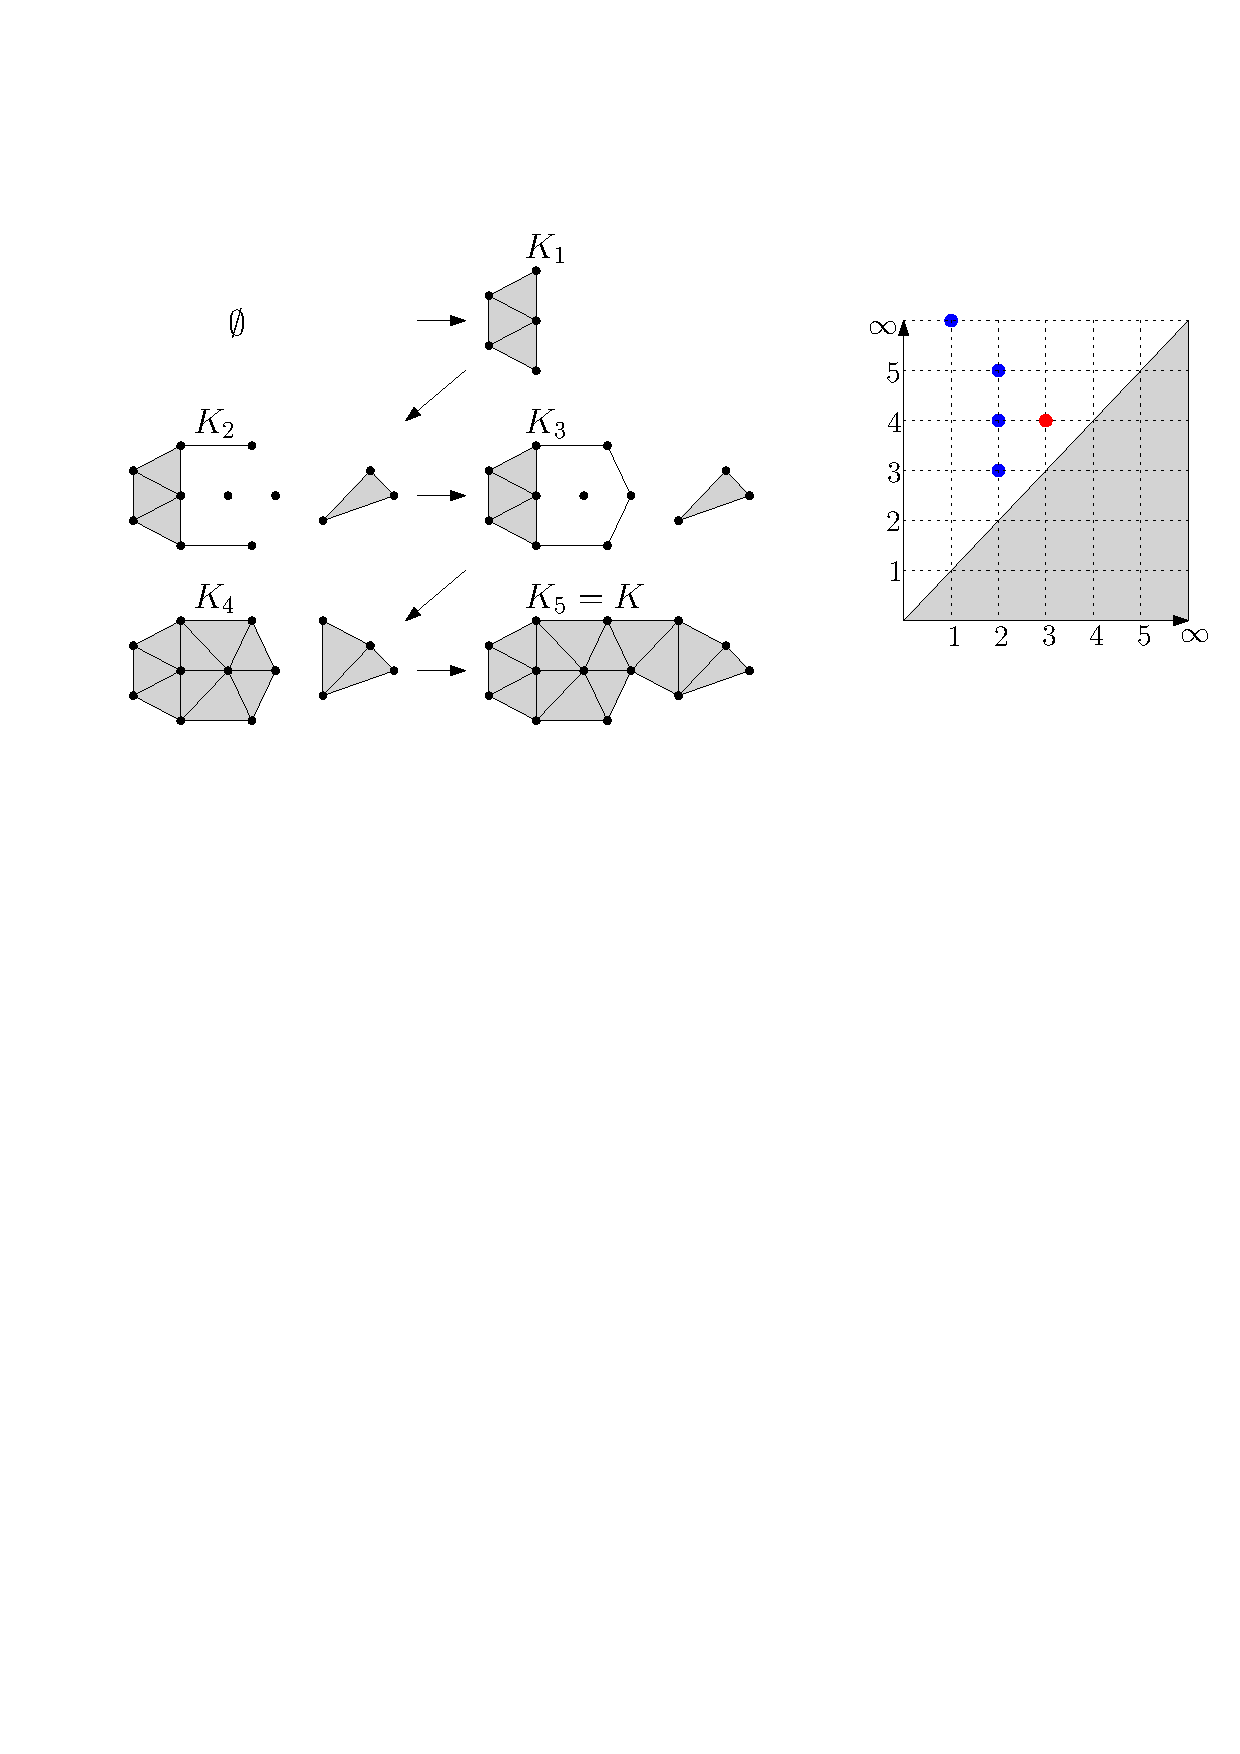
\includegraphics[width = 10cm]{figures/ExampleFiltration} \caption[Persistence diagram induced by filtration]{\label{fig:filtrex} Example of a filtration
and its corresponding persistence diagram (0-dimensional points are marked in blue and 1-dimensional points in red).} 
\end{figure} 

%\begin{figure}[h] \centering 
%\includegraphics[width = 7cm]{figures/Figure_10.pdf} \caption{\label{fig:PDs}
%0th persistence diagram (left) and 1st persistence diagram (right).} 
%\end{figure}

%An important part of persistent theory, which deals with the 
%\textit{stability} of the persistent diagrams, has to be covered. 
%This will done at the beginning of the next chapter, to show how useful it is in our applications. 
%Before moving to the next chapter, 

\paragraph*{Computation.}
The persistence diagram of filtrations of simplicial complexes can be computed with Algorithm~\ref{alg:pers} below, when $\mathbb{K}=\mathbb{Z}_{2}$, 
and when the filtration $\{K_{i}\}_{1\leq i\leq n}$ is such that there is a simplex $\sigma_i$ for which 
$K_{i+1}=K_{i}\cup\{\sigma_{i}\}$ for each $i$. In Algorithm~\ref{alg:pers}, $M$ is the $n\times n$ matrix such that 
$m_{ij}=1\Leftrightarrow\ \sigma_{i}$ is a $({\rm dim}(\sigma_j)-1)$-face of $\sigma_j$, $m_{ij}=0$ otherwise. 
$M_{i}$ is the $i$th column of $M$, and $l_{i}$ is the index of the lowest positive element in $M_{i}$, where $l_i=-1$
by convention when $M_i=0$.

\begin{algorithm}
\caption{\label{alg:pers}  Computation of the persistence diagram}
\begin{algorithmic}
\STATE {\bfseries Input:} $\{K_{i}\}_{1\leq i\leq n}$.
\FOR{$i=0,\cdots,n$} 
	\WHILE{$\exists j<i$ such that $l_{j}==l_{i}\neq -1$} 
		\STATE $M_{i}=M_{i}+M_{j}$ in $\mathbb{Z}_2$
	\ENDWHILE
\ENDFOR
\STATE {\bfseries Output:} $\dg=\sqcup_{i=1}^n\{(l_i,i)\}$.
\end{algorithmic}
\end{algorithm}  

Even though this algorithm has cubic complexity $n^{3}$---see~\cite{Morozov08}, 
faster algorithms can be used in practice depending on the application. 
For instance, 0-dimensional persistent homology in $\mathbb{Z}_{2}$ amounts to track the 
evolution of the connected components, and there exists a very efficient data 
structure that allows to update the number of connected components in a filtration: 
the Union-Find data structure (see Chapter I.1. of~\cite{Edelsbrunner10} for more details). 
This is the data structure we use in practice when we compute 0-dimensional persistent homology.


\subsection{Stability Properties of Persistence Diagrams}\label{sec:stabilityPD}

In this section, we introduce the main property of persistence diagrams, i.e. their {\em stability}
with respect to perturbations of their modules. 
But before presenting the main theorem, we have to detail the metrics we 
are going to use on the persistence modules and their diagrams. 
We start with the metric between persistence modules.

\paragraph*{The interleaving distance.} The so-called {\em interleaving distance}
between persistence modules measures the degree of {\em interleaving}, i.e. the smallest
shift of indices for which one can find commutative diagrams between the modules. 

\begin{defin} 
Two persistence modules $\mathbb{U}$ and $\mathbb{V}$ are \textit{$\epsilon$-interleaved} if there 
exist two families of morphisms $\Psi=\{\psi_{\alpha}:U_{\alpha}\rightarrow V_{\alpha+\epsilon}\,:\, \alpha\in\mathbb{R}\}$ 
and $\Phi=\{\phi_{\alpha}:V_{\alpha}\rightarrow U_{\alpha+\epsilon}\, :\, \alpha\in\mathbb{R}\}$ such that: 
$$\forall\alpha,\epsilon\in\mathbb{R},\epsilon>0,u_{\alpha-\epsilon}^{\alpha+\epsilon}=\phi_{\alpha}\circ\psi_{\alpha-\epsilon}$$ 
$$\forall\alpha,\epsilon\in\mathbb{R},\epsilon>0,v_{\alpha-\epsilon}^{\alpha+\epsilon}=\psi_{\alpha}\circ\phi_{\alpha-\epsilon}$$ 
$$\forall\alpha,\beta,\epsilon\in\mathbb{R},\alpha\leq\beta,\epsilon>0,\psi_{\beta}\circ u_{\alpha}^{\beta}=v_{\alpha+\epsilon}^{\beta+\epsilon}\circ\psi_{\alpha}$$ 
$$\forall\alpha,\beta,\epsilon\in\mathbb{R},\alpha\leq\beta,\epsilon>0,\phi_{\beta}\circ v_{\alpha}^{\beta}=u_{\alpha+\epsilon}^{\beta+\epsilon}\circ\phi_{\alpha}.$$ 
It is equivalent to saying that the diagrams in Figure~\ref{fig:comm} \textit{commute}. 
\end{defin}

\begin{figure}[h] \centering 
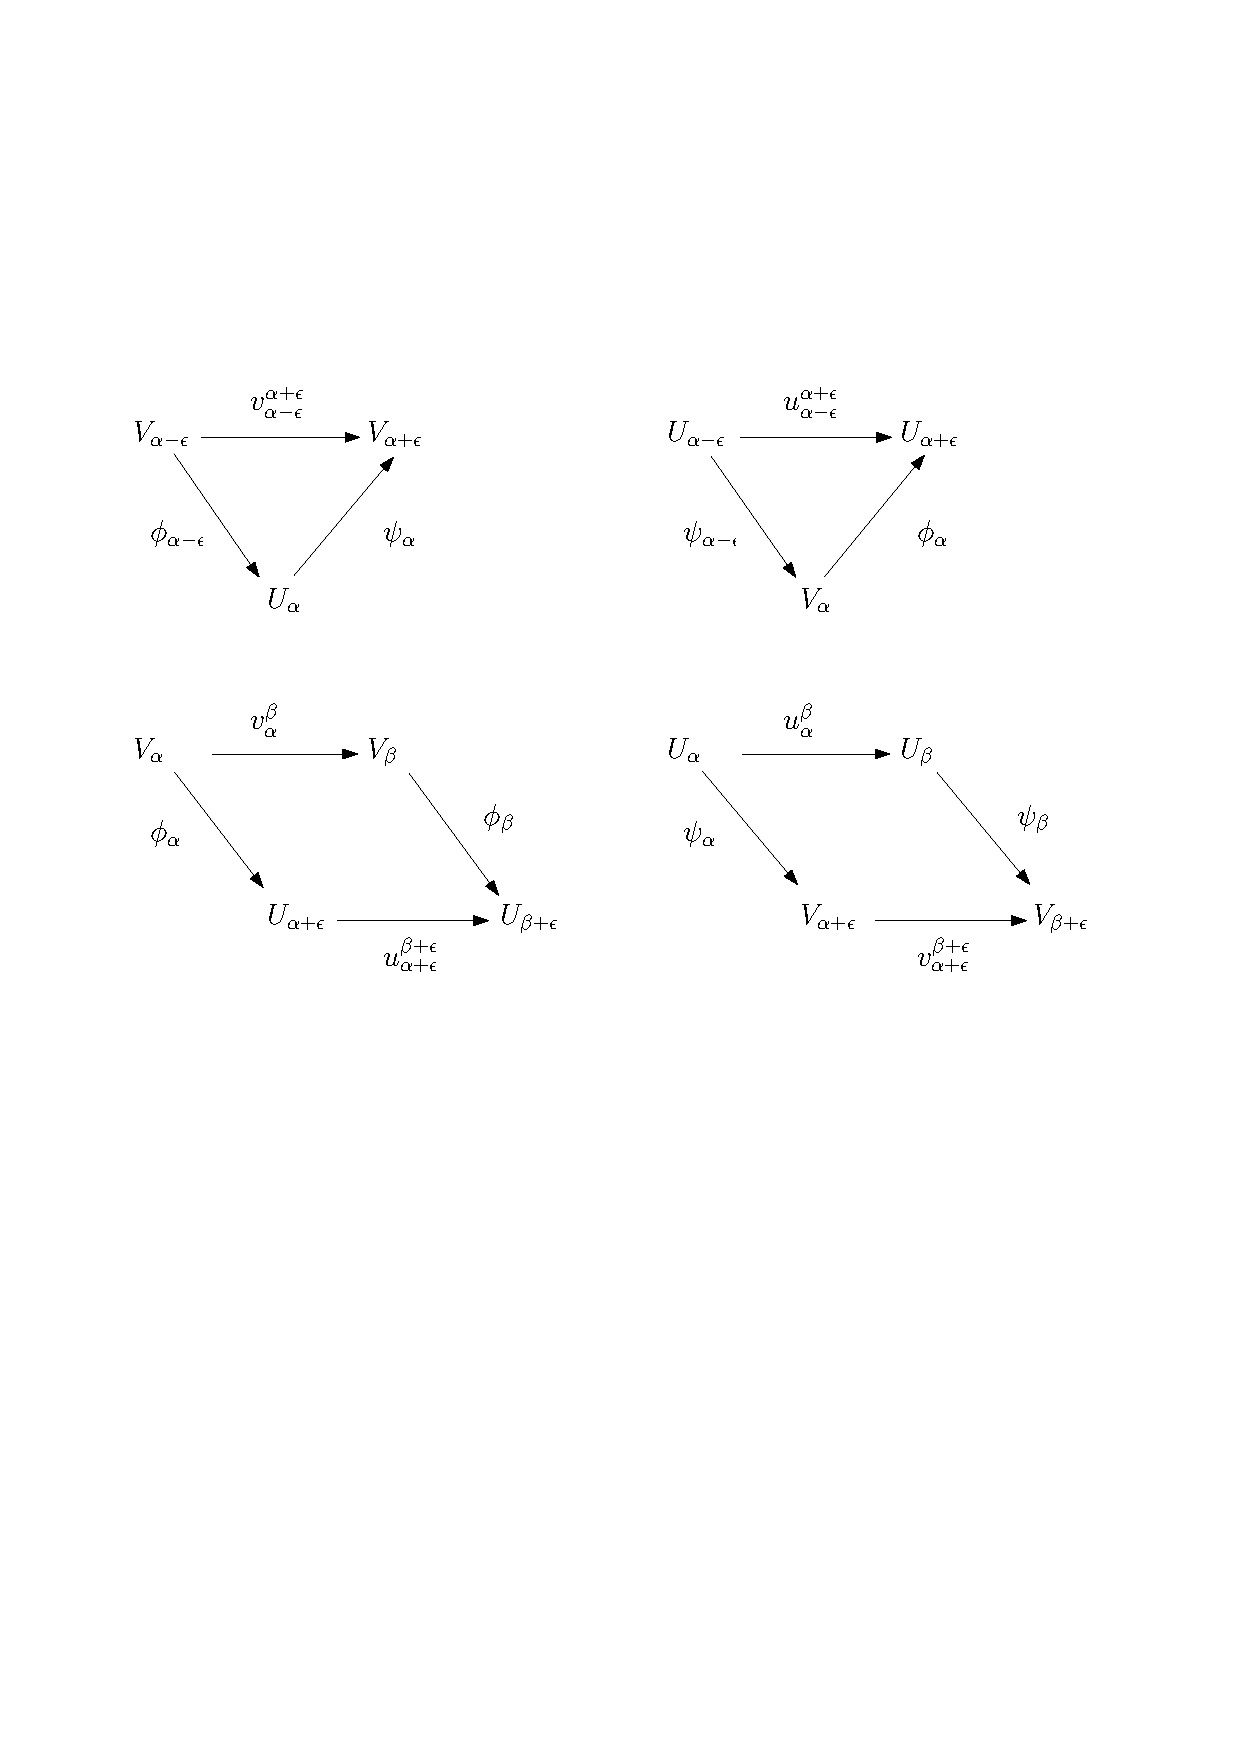
\includegraphics[width = 10cm]{figures/CommutativeDiagrams} \caption{\label{fig:comm}Commutative diagrams for interleaving.} 
\end{figure}

\begin{defin} 
The \textit{interleaving distance $d_{\rm int}$} between two persistence modules is defined by: 
$$\distint(\mathbb{U},\mathbb{V})=\inf\ \{\epsilon\geq 0\,:\, \mathbb{U},\mathbb{V}\text{ are $\epsilon$-interleaved}\}.$$
\end{defin}

\paragraph*{The bottleneck distance.} We now define the distance between persistence diagrams, called the {\em bottleneck distance}.
The definition of this distance is based on partial matchings between the
diagrams. Given two persistence diagrams $\dg,\dg'$, a 
{\em partial matching} between $\dg$ and $\dg'$ is a subset $\Gamma$ of $\dg\times \dg'$ such that:
%
\[
\forall p\in \dg, \text{ there is at most one }p'\in \dg'\text{ such that }(p,p')\in\Gamma,
\]
\[
\forall p'\in \dg', \text{ there is at most one }p\in \dg\text{ such that }(p,p')\in\Gamma.
\]
%
The {\em cost} of $\Gamma$ is:
%
$$\text{cost}(\Gamma)=\max\left\{ \sup_{(p,p')\in\Gamma}\ \|p-p'\|_\infty,
\sup_{p\in\dg\setminus\Gamma}\ \|p-\pi_\Delta(p)\|_\infty,\sup_{p'\in\dg'\setminus\Gamma}\ \|p'-\pi_\Delta(p')\|_\infty\right\},
%\max\left\{\sup_{p\in \dg}\ \delta_{\dg}(p),\ \sup_{p'\in \dg'}\ \delta_{\dg'}(p')\right\},
$$
where, by a slight abuse of notation, we let $\dg\setminus\Gamma$ denote the set of those points in $\dg$ which
have no match in $\Gamma$, and similarly for $\dg'\setminus\Gamma$.
%
%where
%
%\[
%\delta_{\dg}(p)=\|p-p'\|_\infty \text{ if } \exists p'\in \dg'\text{ such that }(p,p')\in\Gamma \text{ and } \delta_{\dg}(p)=d_\infty(p,\Diag)=\inf_{q\in\Diag} \|p-q\|_\infty \text{ otherwise},
%\]
%\[
%\delta_{\dg'}(p')=\|p-p'\|_\infty \text{ if } \exists p\in \dg\text{ such that }(p,p')\in\Gamma \text{ and } \delta_{\dg'}(p')=d_\infty(p',\Diag)=\inf_{q\in\Diag} \|p'-q\|_\infty \text{ otherwise}.
%\]
%
\begin{defin}
\label{def:bottleneck}
Let $\dg,\dg'$ be two persistence diagrams.
The {\em bottleneck distance} between $\dg$ and $\dg'$ is:
%
\[
\distb(\dg,\dg')=\inf_{\Gamma}\ \emph{cost}(\Gamma),
\]
%
where $\Gamma$ ranges over all partial matchings between $\dg$ and $\dg'$.
\end{defin}
%
Note that $\distb$ is only a pseudometric, not a true metric, because points lying on $\Diag$ can be left unmatched at no cost.

\paragraph*{The Wasserstein distances.} In addition to $\distb$, it is possible to define a 1-parameter family of metrics for persistence diagrams by
using the following 1-parameter family of cost functions:
\[
\text{cost}_q(\Gamma)=\left(\sum_{(p,p')\in\Gamma}\|p-p'\|_\infty^q + \sum_{p\in\dg\setminus \Gamma}\|p-\pi_\Delta(p)\|_\infty^q +
\sum_{p'\in\dg'\setminus \Gamma}\|p'-\pi_\Delta(p')\|_\infty^q\right)^{1/q},
\]
for any fixed $q\in\N^*$. This is the definition of the {\em $q$-Wasserstein distance} $\distw{q}$:
$$\distw{q}(\dg,\dg')=\inf_\Gamma\ {\rm cost}_q(\Gamma).$$
%Intuitively, it corresponds to taking taking the sum of the  instead of a max, as in the bottleneck distance.
%is sometimes useful, as we will see in Chapter~\ref{chap:LearningPDs}, where  
%we study the 1-Wasserstein distance.

%\textbf{Example 3.1.} In Figure 4.2, the partial matching $\Gamma$ is 
%$\Gamma=\{(x_{1},y_{1})\}$. 
%\begin{figure}[h]\centering 
%\includegraphics[width = 5cm]{Figure_15.pdf} \caption{Example of partial matching} 
%\end{figure}

%\begin{defin} 
%The \textit{bottleneck distance $\distb$} between two persistence diagrams is defined by: 
%$$\distb(\Dg(\mathbb{U}),\Dg(\mathbb{V}))=\inf\ \{\epsilon>0\,:\,\text{there is an $\epsilon$-partial matching between } \Dg(\mathbb{U}),\Dg(\mathbb{V})\}$$ 
%\end{defin}

\begin{thm}[Theorem 5.14 in~\cite{Chazal16a}]  
Let $\mathbb{U}$ and $\mathbb{V}$ be two decomposable persistence modules. 
Then we have the following inequality: 
\begin{equation} 
\distb(\dg(\mathbb{U}),\dg(\mathbb{V})) = d_{\rm int}(\mathbb{U},\mathbb{V})
\end{equation}
\end{thm}

Note that there exists a similar stability theorem for the Wasserstein distances:

\begin{thm}[Theorem 3.8 in~\cite{Oudot15}]  
Let $\mathbb{U}$ and $\mathbb{V}$ be two decomposable persistence modules. 
Then we have the following inequality: 
\begin{equation} 
\distw{q}(\dg(\mathbb{U}),\dg(\mathbb{V})) \leq ({\rm Pers}(\mathbb{U}) + {\rm Pers}(\mathbb{V}))^{\frac 1q} d_{\rm int}(\mathbb{U},\mathbb{V})^{1-\frac 1q},
\end{equation}
where ${\rm Pers}(\mathbb{U})=\sum_{p\in\dg(\mathbb{U})} 2\|p-\pi_\Delta(p)\|_\infty$.
\end{thm}

%This inequality can actually be turned into an equality---see Theorem~5.14 in~\cite{Chazal16a}.

\paragraph*{Sublevel sets of functions.} An interesting special case is when the persistence modules $\mathbb{U}$ and $\mathbb{V}$ come 
from the filtrations $\{F_{\alpha}\}_{\alpha\in\R}$ and $\{G_{\alpha}\}_{\alpha\in\R}$ induced respectively by tame functions $f$ and $g$ 
on the same topological space $X$. Let $\dg(f)$ and $\dg(g)$ denote the corresponding persistence diagrams, and 
let $\|f-g\|_{\infty}=\sup\{|f(x)-g(x)|\,:\,x\in X\} \leq\epsilon$. 
%We write $\Dg_{i}(f)$ and $\Dg_{i}(g)$ for the $i$th persistence diagrams obtained by their induced filtrations. 
Then, $\forall\alpha\in\mathbb{R}$, $F_{\alpha-\epsilon}\subseteq G_{\alpha}\subseteq F_{\alpha+\epsilon}$ and 
$G_{\alpha-\epsilon}\subseteq F_{\alpha}\subseteq G_{\alpha+\epsilon}$. Indeed, let $x\in X$. 
Then, $f(x)\leq\alpha\ \Rightarrow\ g(x)\leq f(x)+\epsilon\leq\alpha+\epsilon$. The 
inclusion maps $F_{\alpha}\hookrightarrow G_{\alpha+\epsilon}$ and $G_{\alpha}\hookrightarrow F_{\alpha+\epsilon}$ 
induce an $\epsilon$-interleaving at the homology level. Hence, the interleaving distance is bounded by $\epsilon$,
which allows to state the following {\em stability theorem}:

\begin{thm}\label{th:Stab}
Let $X$ be a topological space and $f,g:X\rightarrow\R$ be tame functions.
Then: 
\begin{align}
\distb(\dg(f),\dg(g)) & \leq \|f-g\|_{\infty} \label{eq:Stabbottle} \\
\distw{q}(\dg(f),\dg(g)) & \leq ({\rm Pers}(f)+{\rm Pers}(g))^{\frac 1q}\|f-g\|_{\infty}^{1-\frac 1q} \label{eq:Stabwasser}
\end{align}
\end{thm}

This result is very useful: if one considers a function $f$ and a perturbed version thereof, 
then the persistence diagrams will be stable in the sense that their bottleneck or Wasserstein distances will be less 
than the amplitude of the perturbation. Note that Theorem~\ref{th:Stab} is significantly  
weaker for $\distw{1}$ since, in that case, the upper bound in~(\ref{eq:Stabwasser}) does not depend on $\|f-g\|_\infty$ anymore. 

\paragraph*{Application on point clouds.} An application of Theorem~\ref{th:Stab} is the stability of persistence diagrams
built from growing balls, as in Figure~\ref{fig:ExamplePersistence}. It is stated with the so-called {\em Hausdorff distance}.

\begin{defin}
Let $Y,Z$ be two subsets of a metric space $(X,d_X)$.
Then, the {\em Hausdorff distance} between $Y$ and $Z$ is:
\begin{equation}
\disth(Y,Z)=\max\{\sup_{y\in Y}\inf_{z\in Z}d_X(y,z),\sup_{z'\in Z}\inf_{y'\in Y}d_X(z',y')\}.
\end{equation}  
\end{defin}

\begin{thm}\label{th:StabCech}
Let $P,P'$ be two finite point clouds in a metric space $(X,d_X)$. 
Let $d_P,d_{P'}:X\rightarrow\R_+$ be the distance functions to these point clouds.
Then, $$\distb(\dg(d_P),\dg(d_{P'}))\leq \|d_P-d_{P'}\|_\infty \leq \disth(P,P').$$
\end{thm}


%\paragraph*{Functions defined on different domains.} 
%\begin{thm}
%\label{th:stabilityPD}
%Let $X$ and $Y$ be two  with convexity radii $\rho_X$ and $\rho_Y$ respectively, and let $x\in X$ and $y\in Y$.
%Let $f_x:X\rightarrow\R$ and $f_y:Y\rightarrow\R$ be the corresponding distance functions. 
%Let $\dg_1$ and $\dg_2$ be the PDs associated to the center points $p_1$ and $p_2$ as described in Section~\ref{sec:Def}. 
%Let $C$ be a correspondence between $X$ and $Y$ of metric distortion $\epsilon$ such that $(x,y)\in C$.
%If $\distgh(X,Y)\leq \frac{1}{20}\min\{\rho_X,\rho_Y\}$ and $\e\leq \frac{1}{10}\min\{\rho_X,\rho_Y\}$, then:
%Under some mild conditions on the shapes and $\epsilon$ (stated in~\cite{Carriere15b}), one has: 
%\begin{equation} 
%\distb(\dg(f_x),\dg(f_y))\leq 20\epsilon 
%\end{equation} 
%\end{thm}


%Note that, compared to the stability results of Chapter~\ref{chap:backgroundHomologyPersistence}, 
%for topological signatures, such as the ones
%from~\cite{Chazal09,Chazal13}, 
%this result applies to signatures
%derived from single points on a shape rather than from the entire
%shape itself, which adds a level of difficulty in the analysis.

\section{Extended and Levelset Zigzag Persistence}\label{sec:extendedzigzag}

In this section, we present two extensions of persistent homology, called respectively {\em extended persistence}
and  {\em levelset zigzag persistence}. It turns out that they actually encode the same information---see Corollary~\ref{cor:EPZZ}.
However, we use them both in the following chapters of this thesis, since, depending on the type of result we want to prove,
the one or the other can be easier to work with. Again, we define these objects for topological spaces, 
but the definitions hold for simplicial complexes as well.

\paragraph*{Notation.} From now, on, given a real-valued function $f$ on a topological space $X$, and an
interval $I\subseteq\R$, we denote by $X_f^I$ the preimage
$f^{-1}(I)$. We omit the subscript $f$ in the notation when there is
no ambiguity in the function considered.

\subsection{Extended persistence}\label{sec:extended}

%\paragraph*{Convention.} In this Section, homology groups are always computed with $\Z_2$ coefficients, so we do not
%specify the field of coefficient in their notation.


\paragraph*{Filtrations with superlevel sets.} 
Let $f$ be a real-valued function on a topological space $X$.
%The family $\{X^{(-\infty, \alpha]}\}_{\alpha\in\R}$ of
%sublevel sets of $f$ defines a {\em filtration}, that is, it is
%nested with respect to the inclusion: $X^{(-\infty, \alpha]}\subseteq
%X^{(-\infty, \beta]}$ for all $\alpha\leq\beta\in\R$. 
Recall that the family of sublevel sets of $f$ is nested, and induces a filtration of $X$.
The family $\{X^{[\alpha, +\infty)}\}_{\alpha\in\R}$ of superlevel sets of $f$ is also
nested but in the opposite direction: $X^{[\alpha, +\infty)}\supseteq X^{[\beta, +\infty)}$
for all $\alpha\leq\beta\in\R$. We can turn it into a filtration by
reversing the real line. Specifically, let $\Rop=\{\tilde{x}\,:\,x\in\R\}$,
ordered by $\tilde{x}\leq\tilde{y}\Leftrightarrow x\geq y$. We index
the family of superlevel sets by $\Rop$, so now we have a
filtration: $\{X^{[\tilde\alpha, +\infty)}\}_{\tilde\alpha\in\Rop}$, with
$X^{[\tilde\alpha, +\infty)}\subseteq X^{[\tilde\beta, +\infty)}$ for all
$\tilde\alpha\leq\tilde\beta\in\Rop$.

\paragraph*{Extended filtration.} Extended persistence connects the two filtrations at infinity as
follows. Replace each superlevel set $X^{[\tilde\alpha, +\infty)}$ by
the pair of spaces $(X, X^{[\tilde\alpha, +\infty)})$. This maintains the filtration property since we have
$(X, X^{[\tilde\alpha, +\infty)})\subseteq (X, X^{[\tilde\beta,+\infty)})$ for all
$\tilde\alpha\leq\tilde\beta\in\Rop$. Then, let
$\Rext=\R\cup\{+\infty\}\cup\Rop$, where the order is
completed by $\alpha<+\infty<\tilde{\beta}$ for all
$\alpha\in\R$ and $\tilde\beta\in\Rop$. %This poset is
%isomorphic to $(\R, \leq)$. 
Finally, define the {\em extended filtration} of $f$ over $\Rext$ by:
%
\[
\begin{array}{llll}
F_\alpha &=& X^{(-\infty, \alpha]} & \mbox{for $\alpha\in\R$}\\[0.5em]
F_{+\infty} &=& X \equiv (X,\emptyset)\\[0.5em]
F_{\tilde\alpha} &=& (X, X^{[\tilde\alpha, +\infty)}) & \mbox{for $\tilde\alpha\in\Rop$},
\end{array}
\]
%
where we have identified the space $X$ with the pair of spaces $(X,\emptyset)$. 
This is a well-defined filtration since we have
$X^{(-\infty, \alpha]}\subseteq X \equiv (X, \emptyset) \subseteq (X,X^{[\tilde\beta, +\infty)})$ 
for all $\alpha\in\R$ and $\tilde\beta\in\Rop$.  The subfamily $\{F_\alpha\}_{\alpha\in\R}$ is
called the {\em ordinary} part of the filtration, and the
subfamily $\{F_{\tilde\alpha}\}_{\tilde\alpha\in\Rop}$ is called the
{\em relative} part. See Figure~\ref{fig:ExFilt} for an illustration.

%%%
\begin{figure}[htb]
\begin{center}
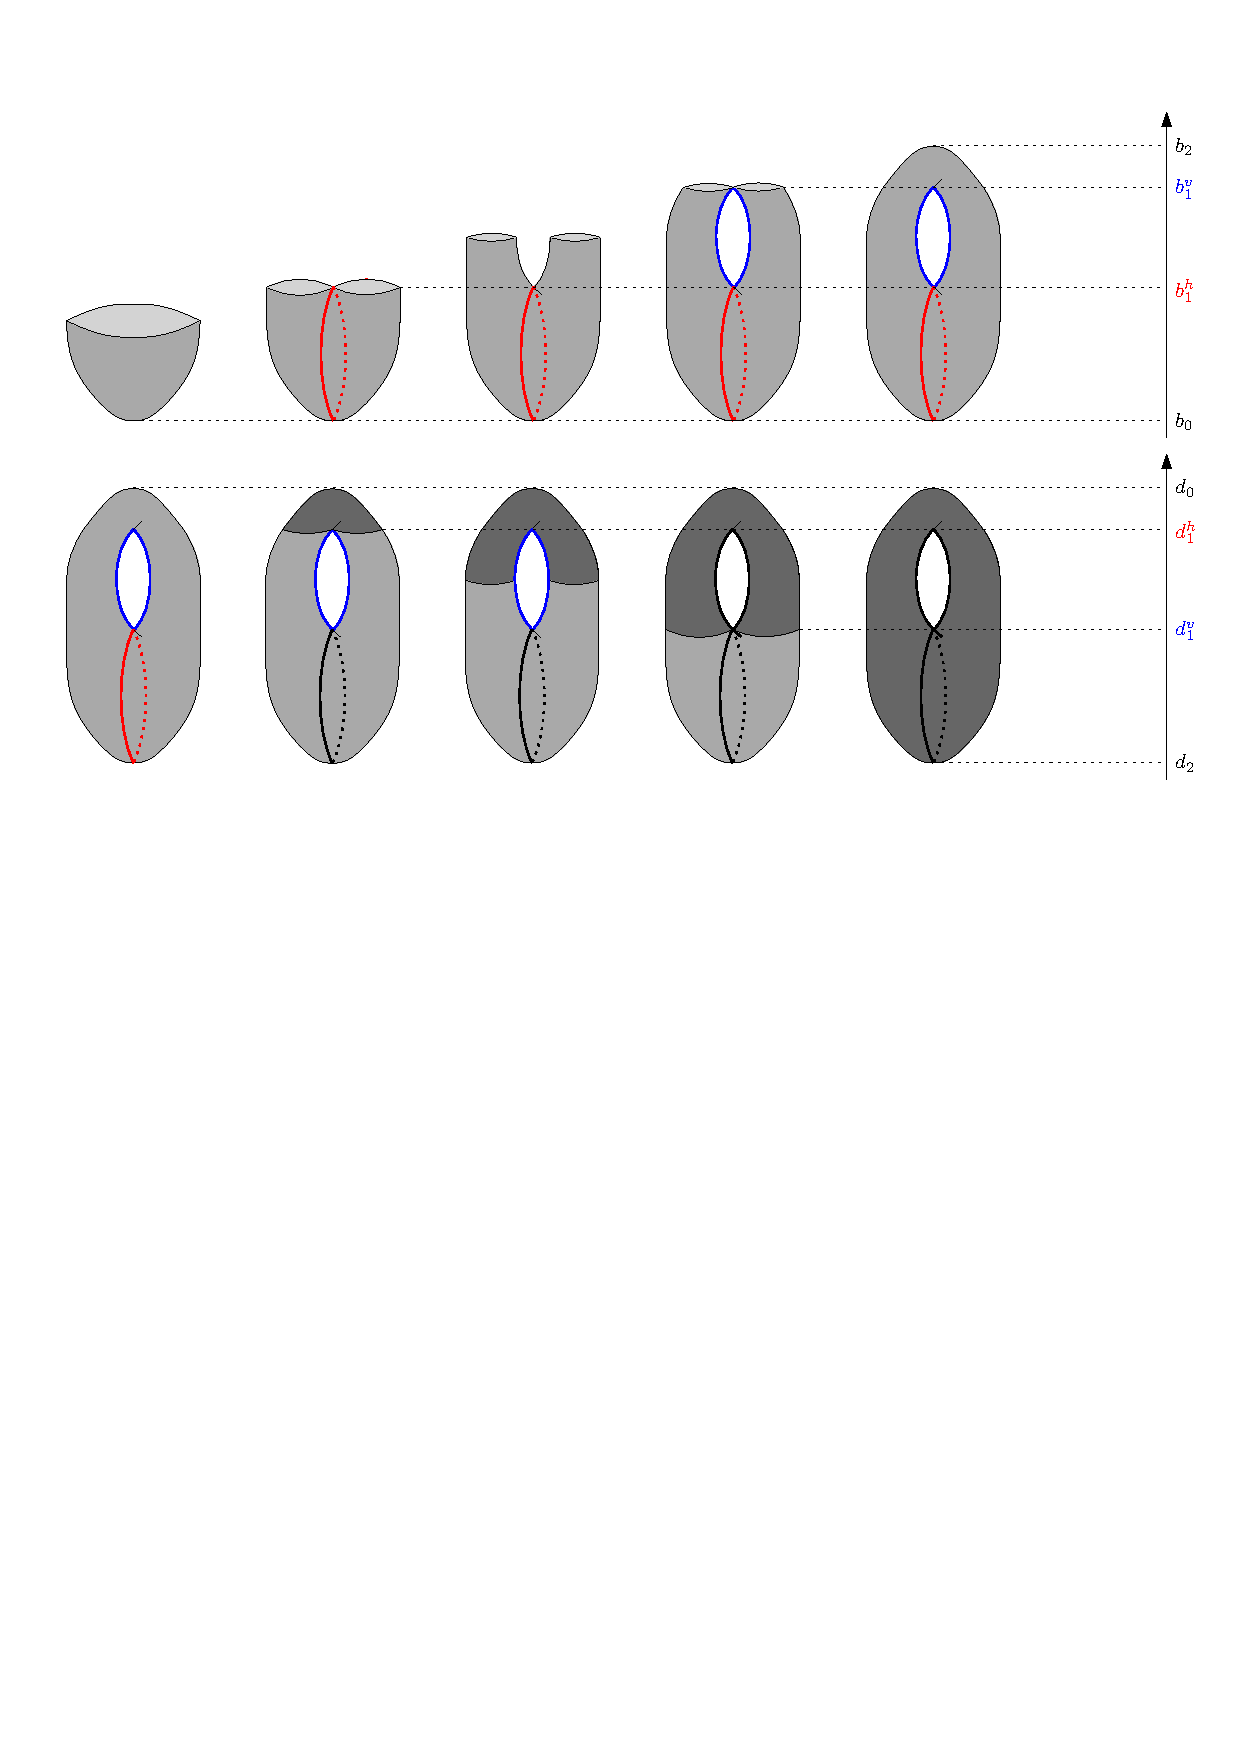
\includegraphics[width=13cm]{figures/ExFilt}
\caption[Extended filtration]{\label{fig:ExFilt} The extended filtration of the
height function on a torus.  The upper row displays the ordinary
part of the filtration while the lower row displays the relative part.  
The red and blue cycles both correspond to
extended points in dimension 1.  The point corresponding to
the red cycle, sometimes called {\em horizontal cycle}, is located above 
the diagonal ($d_1^h>b_1^h$), while
the point corresponding to the blue cycle, sometimes called {\em vertical cycle},  
is located below the
diagonal ($d_1^v>b_1^v$).}
\end{center}
\end{figure}

\paragraph*{Extended persistence module.} 
%Applying the homology functor $\Hom_*$ to this filtration gives 
Inclusions in the extended filtration induce the so-called {\em extended persistence module} $\EP(f)$:
%
\[
\begin{array}{llll}
\EP(f)_\alpha &=& H_*(F_\alpha;\mathbb K)=H_*(X^{(-\infty, \alpha]};\mathbb K) & \mbox{for $\alpha\in\R$}\\[0.5em]
\EP(f)_{+\infty} &=& H_*(F_{+\infty};\mathbb K)=H_*(X;\mathbb K) \cong H_*(X,\emptyset;\mathbb K)\\[0.5em]
\EP(f)_{\tilde\alpha} &=& H_*(F_{\tilde\alpha};\mathbb K)=H_*(X, X^{[\tilde\alpha, +\infty)};\mathbb K) & \mbox{for $\tilde\alpha\in\Rop$}.
\end{array}
\]
%
%and where the linear maps between the spaces are induced by the
%inclusions in the extended filtration.



\paragraph*{Decomposition.} As for ordinary persistence, an extended persistence module can be
decomposed as a direct sum of interval modules whenever the function $f$ is tame, meaning
%that the morphisms between 
that the (relative) homology groups %, either relative or not, 
of its sub- or superlevel sets are finite-dimensional---see e.g. Section 6.2 in~\cite{Chazal16a}:
%
\[
\EP(f)\simeq\bigoplus_{\alpha\in A} \mathbb{I}[b_\alpha, d_\alpha),
\]
%
where $A$ is an index set, where $b_\alpha\leq d_\alpha\in\Rext$,
and where each summand $\mathbb{I}[b_\alpha, d_\alpha)$ is made of copies of $\mathbb K$ 
at each index $\beta\in [b_\alpha, d_\alpha)$, and of
copies of the zero space elsewhere, the maps between copies of $\mathbb K$ being identities. 

\paragraph*{Extended persistence diagram.}
Given a tame function $f$, its extended persistence module can be encoded in the so-called {\em extended persistence diagram} $\Dg(f)$.  
%Each summand represents the lifespan of a
%{\em homological feature} (connected component, hole, void, etc.) within the
%filtration. More precisely, the {\em birth time} $b_i$ and {\em death time} 
%$d_i$ of the feature are given by the endpoints of
%the interval.  Then, a convenient way to represent the structure
%of the module is to plot each interval in the decomposition as a
%oint in the extended plane, whose coordinates are given by the
%endpoints. Such a plot is called the {\em extended persistence diagram} of $f$, 
%denoted $\Dg(f)$.  
Moreover, the distinction
between ordinary and relative parts of the filtration allows to
classify the points in $\Dg(f)$ in the following way:
%
\begin{itemize}
\item points whose coordinates both belong to $\R$  are called {\em ordinary} points; 
they correspond to homological features being born and then dying in the ordinary part of the filtration;
\item points whose coordinates both belong to $\Rop$ are called {\em relative} points; 
they correspond to homological features being born and then dying in the relative part of the filtration;
\item points whose abscissa belongs to $\R$  and whose ordinate belongs to $\Rop$ are called {\em extended} points; 
they correspond to homological features being born in the ordinary part and then dying in the relative part of the filtration. 
\end{itemize}
%
Note that ordinary points lie strictly above the diagonal
$\Diag=\{(x,x)\,:\,x\in\bar\R\}$ and relative points lie strictly below $\Diag$,
while extended points can be located anywhere, including on $\Diag$ (e.g. for connected components 
lying inside a single critical level).  It is common to
decompose $\Dg(f)$ according to this classification:
%
\[
\Dg(f)=\Ord(f)\sqcup\Rel(f)\sqcup\Ext^+(f)\sqcup\Ext^-(f),
\]
%
where by convention $\Ext^+(f)$ includes the extended points located on the diagonal~$\Diag$.

\paragraph*{Persistence measure.}

From an extended persistence module ${\rm EP}(f)$ we derive a measure on the set of rectangles in the plane, 
called the \textit{persistence measure} and denoted $\mu_{\rm EP}$. Given a rectangle~$R=[a,b]\times[c,d]$ with $a<b\leq c<d\in\Rext$, we let 
%
\begin{equation}\label{eq:pers_meas}
\mu_{\rm EP}(R)=r_b^c-r_b^d+r_a^d-r_a^c,
\end{equation}
%
where $r_x^y$ denotes the rank of the linear map between the vector
spaces indexed by $x,y\in\R_{\Ext}$ in~$\EP(f)$.
When $\EP(f)$ has a well-defined persistence diagram, i.e. $f$ is tame, $\mu_{\EP}(R)$ equals the total 
multiplicity of the diagram within the rectangle~$R$~\cite{Chazal16a}.

\paragraph*{Stability.}
Extended persistence diagrams are also stable
in the bottleneck and Wasserstein distances:
% 
\begin{thm}[EP Stability Theorem in~\cite{Carlsson09b}]
\label{th:ExStab}
For any  tame functions $f,g:X\rightarrow\R$,
%
\begin{align}
\distb(\Dg(f),\Dg(g)) & \leq \|f-g\|_\infty\\
\distw{q}(\Dg(f),\Dg(g)) & \leq ({\rm Pers}(f)+{\rm Pers}(g))^{\frac 1q}\|f-g\|_\infty^{1-\frac 1q}
\end{align}
%
\end{thm}
%
Moreover, as pointed out in~\cite{Cohen09}, the theorem can be
strengthened to apply to each subdiagram
$\Ord$, $\Ext^+$, $\Ext^-$, $\Rel$ and to each homological dimension
individually.

Extended persistence diagrams also enjoy a {\em symmetry theorem} when $X$ is a $d$-manifold, where $d\in\N^*$.


\begin{thm}[Symmetry Theorem in~\cite{Cohen09}]\label{th:EPsym}
Let $R:(x,y)\mapsto(-x,-y)$. Then,
for any tame function $f:X\rightarrow\R$ defined on a $d$-manifold $X$, one has, for any homological dimension $p <d$:
{\rm (i)} $\Ord_p(f)=R(\Ord_{d-p-1}(-f))$, 
{\rm (ii)} $\Rel_p(f)=R(\Rel_{d-p-1}(-f))$ and 
{\rm (iii)} $\Ext_p(f)=R(\Ext_{d-p}(-f))$.

\end{thm}

%%%%%%%%%%%%%%%%%%%%%%%
\subsection{Levelset zigzag persistence}
\label{sec:ZZ}

Levelset zigzag persistence~\cite{Carlsson09b} is specifically designed for the so-called {\em Morse-type functions} and the 
stratification of the space they induce.

\paragraph*{Morse-type functions.}
%The extended persistence module of a function $f$ can be simplified if the function is {\em of Morse type}.
Morse-type functions are generalizations of the classical Morse
functions that share some of their properties without having to be
differentiable nor defined over a smooth manifold.



\begin{defin}[Morse-type~\cite{Carlsson09b}]\label{def:Morse-type}
A continuous real-valued function $f$ on a topological space $X$ is {\em of Morse type} if:

\begin{itemize}

\item[{\rm (i)}] There is a finite set $\Crit(f)=\{a_1<...<a_n\}$, called the set of {\em critical values},
such that for every open interval $(a_0=-\infty,a_1),...,(a_i,a_{i+1}),...,(a_n,a_{n+1}=+\infty)$
there is a compact and locally connected space $Y_i$ 
and a homeomorphism $\mu_i:Y_i\times(a_i,a_{i+1})\rightarrow X^{(a_i,a_{i+1})}$
such that $\forall i=0,...,n, f|_{X^{(a_i,a_{i+1})}}=\pi_2\circ\mu_i^{-1}$, where
$\pi_2$ is the projection onto the second factor;

\item[{\rm (ii)}] $\forall i=1,...,n-1,\mu_i$ extends to a continuous function $\bar{\mu}_i:Y_i\times[a_i,a_{i+1}]\rightarrow X^{[a_i,a_{i+1}]}$
-- similarly $\mu_0$ extends to $\bar\mu_0:Y_0\times(-\infty,a_1]\rightarrow X^{(-\infty,a_1]}$
and $\mu_n$ extends to $\bar\mu_n:Y_n\times[a_n,+\infty)\rightarrow X^{[a_n,+\infty)}$;

\item[{\rm (iii)}] Each levelset $X^t$ has a finitely-generated homology.

\end{itemize}
\end{defin}

Items~(i) and~(ii) define a stratification of $X$, which we use extensively in the next chapters.
Morse functions are known to be of Morse type while the converse is
clearly not true. Moreover, it follows from item (iii) in Definition~\ref{def:Morse-type} that
Morse-type functions induce tame, and thus decomposable %{\em pointwise finite-dimensional} (pfd) 
extended persistence modules.
%, meaning that each vector space in the extended persistence module has finite dimension. Clearly, pfd persistence modules are tame and thus decomposable.


%Indeed, between any pair of consecutive critical values, there are no homological events, so the persistence module of the function
%should only depend on these critical values.  

\paragraph*{Zigzag persistence modules.} A zigzag persistence module is a discrete persistence module whose arrows can go
indifferently  forward {\em or} backward.

\begin{defin}
Let $\mathbb K$ be a field and $n\in\N$. 
A {\em zigzag persistence module} $\mathbb U$ is a set of $\mathbb{K}$-vector spaces indexed by $\{1,\cdots,n\}$, denoted by
$\{U_i\}_{1\leq i\leq n}$,
together with a family of linear maps $\{u_i:U_i\leftrightarrow U_{i+1}\}_{1\leq i\leq n-1}$, where $\leftrightarrow$
means that the linear map is either $\rightarrow$ or $\leftarrow$.
\end{defin}

As for usual persistence modules, any sequence of topological spaces with canonical inclusions (going either forward or backward) 
induces a zigzag persistence module after computing the homology groups. Note however that the full sequence is not required to be a filtration anymore.
Particular zigzag persistence modules, called {\em levelset zigzag persistence modules}, can be defined for Morse-type functions.

\begin{defin}\label{def:LZZ} 
Let $f:X\rightarrow\R$ be a Morse-type function, 
and let $\Crit(f)=\{a_1,\cdots,a_n\}$ be its set of critical values.
Let $-\infty=a_0<s_0<a_1<s_1<a_2<\cdots<s_{n-1}<a_n<s_n<a_{n+1}=+\infty$. Then, for any $1\leq i \leq j \leq n$, we write $X_i^j$ for $X^{[s_i,s_j]}$,
and we define the {\em levelset zigzag} as the following sequence of $2n+1$ nodes:
$$X_0^0\hookrightarrow X_0^1 \hookleftarrow X_1^1 \hookrightarrow X_1^2 \hookleftarrow \cdots \hookrightarrow X_{n-1}^n \hookleftarrow X_n^n,$$
where each arrow is an inclusion. %Note that this does not define a filtration since the spaces are not nested, i.e. the inclusions
%can go forward {\em and} backward. However, these inclusions still induce a discrete persistence module, called the 
%Applying the homology functor $H_*$ to the levelset zigzag gives 
Computing the homology groups of each space and the linear maps induced from the corresponding inclusions gives the so-called
{\em levelset zigzag persistence module} $\LZZ(f)$:
$$H_*(X_0^0;\mathbb K)\rightarrow H_*(X_0^1;\mathbb K)\leftarrow H_*(X_1^1;\mathbb K) \rightarrow H_*(X_1^2;\mathbb K) 
\leftarrow \cdots \rightarrow H_*(X_{n-1}^n;\mathbb K) \leftarrow H_*(X_n^n;\mathbb K).$$
%In general, we use the term {\em zigzag} to characterize modules whose arrows can go forward {\em and} backward. 
%., where the linear maps between the spaces are induced by the inclusions.
\end{defin}


\paragraph*{Decomposition.} Zigzag persistence modules also enjoy a decomposition theorem: 

\begin{thm}[Theorem 2.5 in~\cite{Carlsson10}]
Any zigzag persistence module $\mathbb U$ decomposes as a direct sum of closed interval modules:
$$\mathbb U\simeq \bigoplus_{\alpha\in A}\mathbb{I}_{[b_\alpha,d_\alpha]},$$ %{[X_{i_k}^{i_k'},X_{j_k}^{j_k'}]},
where $A$ is an index set, where $1\leq b_\alpha\leq d_\alpha\leq n$,
and where each summand $\mathbb{I}_{[b_\alpha, d_\alpha]}$ is made of copies of
$\mathbb K$ at each index $\beta\in [b_\alpha, d_\alpha]$, and of
copies of the zero space elsewhere, the maps between copies of $\mathbb K$ being identities. 
\end{thm}

In the case of a levelset zigzag persistence module induced by a Morse-type function $f$, 
each closed interval $[b_\alpha,d_\alpha]$ is of the form ${[X_{i_\alpha}^{i_\alpha'},X_{j_\alpha}^{j_\alpha'}]}$,
where $i_\alpha'$ is either $i_\alpha$ or $i_\alpha+1$ and similarly for $j_\alpha'$, hence the following classification:
\begin{table}[h]\centering
\begin{tabular}{|l|l|l|l|l|}
\hline
Type & I                                             & II                                            & III                                             & IV \\
\hline
     & \( \begin{array}{l} i_\alpha'=i_\alpha+1 \\ j_\alpha'=j_\alpha \end{array}\)  
     & \( \begin{array}{l} i_\alpha'=i_\alpha \\ j_\alpha'=j_\alpha+1 \end{array}\)   
     & \( \begin{array}{l} i_\alpha'=i_\alpha+1 \\ j_\alpha'=j_\alpha+1\end{array}\)  
     & \( \begin{array}{l} i_\alpha'=i_\alpha \\ j_\alpha'=j_\alpha\end{array}\) \\
\hline
\end{tabular}
\end{table}

%\begin{itemize}
%\item if $i_\alpha'=i_\alpha+1$ and $j_\alpha'=j_\alpha$ the interval is of type I,
%\item if $i_\alpha'=i_\alpha$ and $j_\alpha'=j_\alpha+1$ the interval is of type II,
%\item if $i_\alpha'=i_\alpha+1$ and $j_\alpha'=j_\alpha+1$ the interval is of type III,
%\item if $i_\alpha'=i_\alpha$ and $j_\alpha'=j_\alpha$ the interval is of type IV.
%\end{itemize}
The disjoint union of all of these intervals is called the {\em levelset zigzag persistence barcode} $\DgZZ(f)$.
%We also denote the restriction of $\DgZZ(f)$ to type I intervals as I-$\DgZZ(f)$, and similarly for the other types.
%and where each summand $\mathbb{I}_{I_k}$ %[X_i^{i'},X_j^{j'}]$ 
%is made of copies of $\mathbb K$ for each space between $X_{i_k}^{i_k'}$ and $X_{j_k}^{j_k'}$ and of
%copies of the zero space elsewhere, the maps between copies of the field being identities.

 
%\paragraph*{Levelset zigzag persistence barcode.} Again, each interval in the decomposition of a zigzag persistence module 
%can be associated to a point in the plane to produce a
%{\em zigzag persistence diagram}. 

%However, in the case of levelset zigzag persistence modules, we refine
%this description by distinguishing between the four different types of intervals that may occur in the
%decomposition due to the stratification induced by Morse-type functions.
%%Due to the stratification of Morse-type functions, 
%More precisely, interval modules can be associated to {\em critical intervals} with the following correspondence:
%\begin{align*}
%[X_i^i,X_j^j] & \longleftrightarrow (a_i,a_{j+1}) & [X_i^i,X_j^{j+1}] & \longleftrightarrow (a_i,a_{j+1}] \nonumber\\
%[X_i^{i+1},X_j^j] & \longleftrightarrow [a_{i+1},a_{j+1}) &  [X_i^{i+1},X_j^{j+1}] & \longleftrightarrow [a_{i+1},a_{j+1}]\nonumber
%\end{align*}
%The union of these intervals gives the so-called 
%{\em levelset zigzag persistence barcode} $\DgZZ(f)$.

\paragraph*{Mayer-Vietoris half-pyramid.} Morse-type functions also allow us to build the so-called {\em Mayer-Vietoris half-pyramid}~\cite{Carlsson09b}, 
which is the diagram of topological spaces and inclusions displayed in Figure~\ref{fig:ZZpyramid}.
%We refer the reader to~\cite{Carlsson09b} for more details.
Any zigzag within the Mayer-Vietoris half-pyramid that stretches from the left boundary (i.e. the node $X_0^0)$ 
to the right boundary without backtracking
is called {\em monotone}. Theorem~\ref{th:MY} and Corollary~\ref{cor:EPZZ} below allow us to link the zigzag persistence modules of 
any pair of monotone zigzags in the half-pyramid.
 %come from~\cite{Carlsson09b}, 
We use these results extensively in Section~\ref{sec:topoMultiNerve}.

\begin{figure}\centering
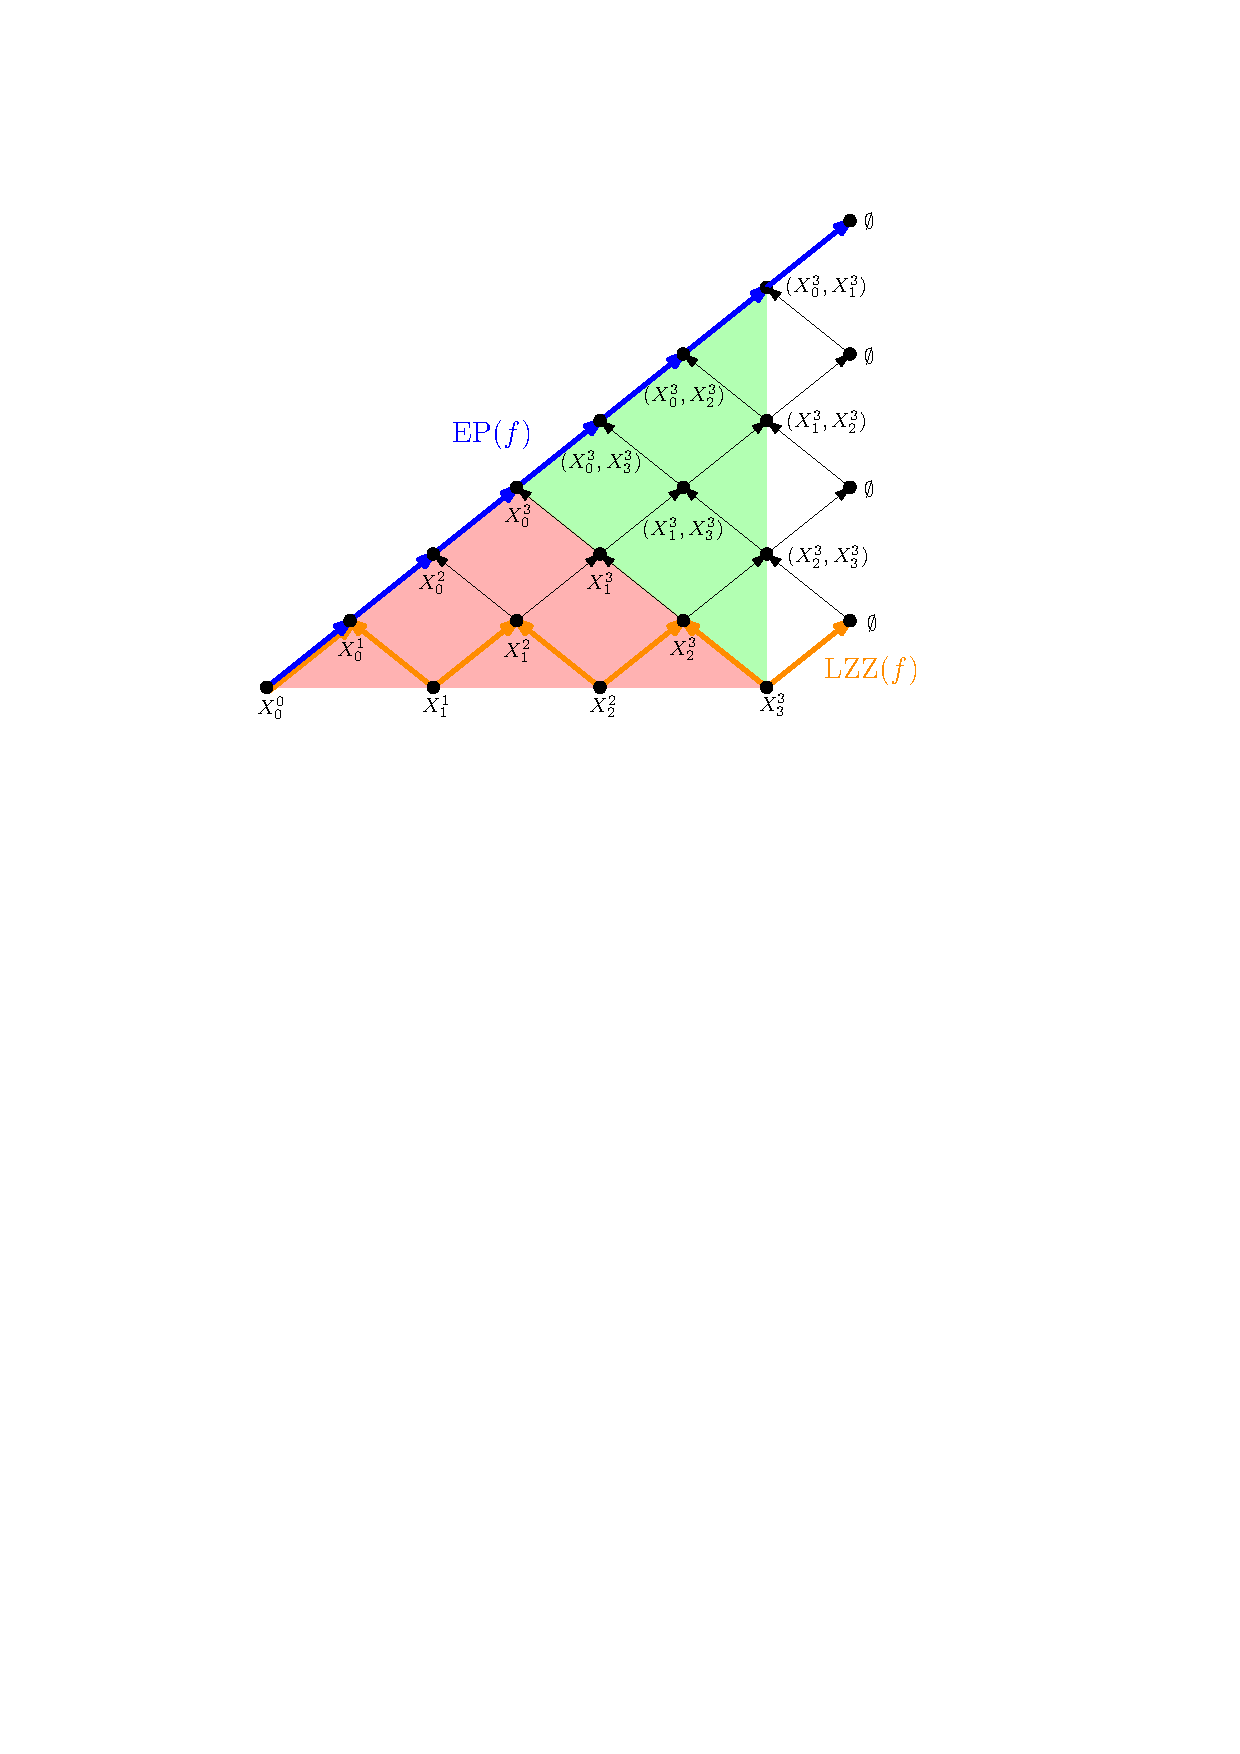
\includegraphics[width=12.5cm]{figures/ZZpyramid}
\caption[Mayer-Vietoris half-pyramid]{\label{fig:ZZpyramid} We show the Mayer-Vietoris half-pyramid when the Morse-type function has
3 critical values. It is composed of two faces of the full Mayer-Vietoris pyramid: 
the south face (red) and the east face (green). The extended persistence module ${\rm EP}(f)$ is in blue and 
the levelset zigzag persistence module $\LZZ(f)$ is in orange.}
\end{figure}

\begin{thm}[Pyramid Theorem in~\cite{Carlsson09b}]\label{th:MY}
For any Morse-type function $f$, there exists a bijection between the barcodes of any pair of monotone zigzag persistence modules in the Mayer-Vietoris half-pyramid.
\end{thm}

Since the extended persistence module of $f$ is a monotone zigzag persistence
module---more precisely the principal diagonal---of the Mayer-Vietoris half-pyramid, we have the following corollary.


\begin{cor}[Table 1 in~\cite{Carlsson09b}]\label{cor:EPZZ}
For any Morse-type function $f$, there exists a bijection between $\Dg(f)$ and $\DgZZ(f)$,
which is described in Table~\ref{tab:EPZZ}.
\end{cor}

\begin{table}[h]\centering
\begin{tabular}{|l|l|l|l|l|}
\hline
Type                      & $\Ord$                         & $\Rel$                      & $\Ext^+$                          & $\Ext^-$                   \\
\hline
$\Dg(f)$                  & $[a_i,a_j)$                    & $[\tilde a_j, \tilde a_i)$  & $[a_i,\tilde a_j)$                & $[a_j, \tilde a_i)$     \\
\hline
\hline
$\DgZZ(f)$                & $[X_{i-1}^i,X_{j-1}^{j-1}]$    & $[X_i^i,X_{j-1}^j]^-$       & $[X_{i-1}^i,X_{j-1}^j]$           & $[X_i^i,X_{j-1}^{j-1}]^-$ \\
\hline
Type                      & I                              & II                          & III                               & IV \\
\hline
\end{tabular}
\caption{\label{tab:EPZZ} This table gives the correspondences between the points of $\Dg(f)$ and the intervals of $\DgZZ(f)$.
The minus sign on some intervals of $\DgZZ(f)$ means that the homological dimension of that interval is equal to the dimension of 
its corresponding point in $\Dg(f)$ minus 1. }
\end{table}
 
In particular, bottleneck and Wasserstein distances, as well as stability results, can be derived for levelset zigzag persistence barcodes using
this correspondence and Theorem~\ref{th:ExStab}.

%%%%%%%%%%%%%%%%%%%%%%%%%%%%%%%%%%%%%%%%%%%%%%%%%%%%%%%%%%%%%%%%%%%%%%%%%%%
\section{Reeb graphs}
\label{sec:reebgraph}



%Since Reeb graphs of Morse-type functions are actually telescopes with 
%1-dimensional cylinders %(obtained from the preimages of a continuous function,
%We have now defined all the tools we need to study.
%In the context of shape analysis, 
The Reeb graph provides a meaningful alternative to persistence diagrams as summary
of a topological space and a real-valued function defined on that space.
Intuitively, it continuously collapses the connected components of the level sets of the function into single points, thus tracking
the values of the functions at which the connected components merge or split.
Reeb graphs have been widely used in computer graphics and visualization---see~\cite{Biasotti08} for a survey. 
%
%In this section, we formally define Reeb graphs and detail the bag-of-feature interpretation of
%extended persistence diagrams computed from Reeb graphs. %in Section~\ref{sec:dictionary}. 
%We then relate the topology of the Reeb graph
%to the one of the original space in Section~\ref{sec:topologyReeb}, and we describe several metrics between the Reeb graphs in Section~\ref{sec:metrics}. 
%
%
%\subsection{Reeb graphs and their persistence diagrams}
%\label{sec:reebdef}
%
\begin{defin}
Given a topological space $X$ and a continuous function 
$f:X\rightarrow\R$, we define the equivalence relation $\sim_f$ between points of $X$ by:
%
\[
x\sim_f y\ \Leftrightarrow\ \left[ f(x)=f(y)\emph{ and }x,y\ \emph{belong to the same connected component of}\ f^{-1}(f(x))=f^{-1}(f(y))\right].
\]
%
The \emph{Reeb graph} $\Reeb_f(X)$ is the quotient space $X/\sim_f$.
\end{defin}
%
%%%
\begin{figure}[htb] 
\begin{center}
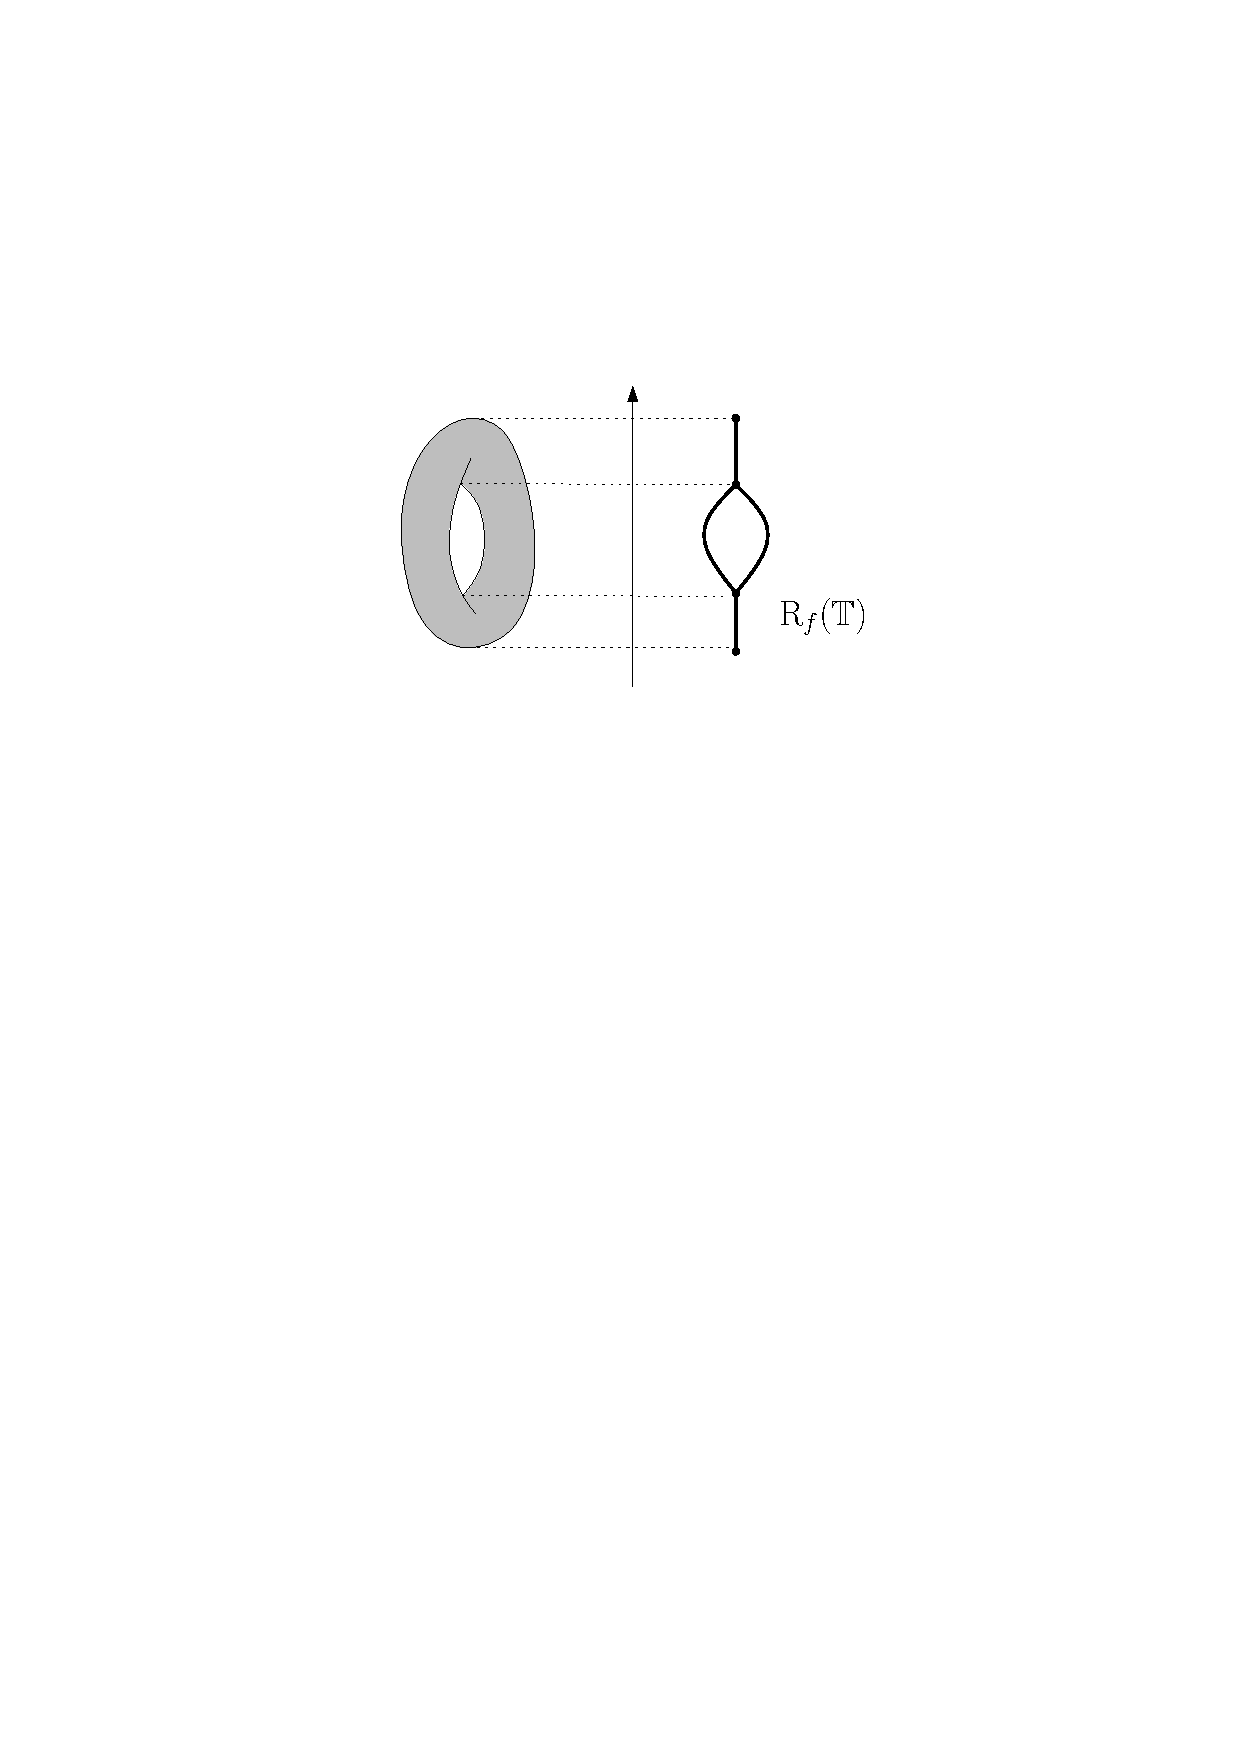
\includegraphics[height = 3.5cm]{figures/ReebGraphTorus}\hspace{3mm}
\caption[Reeb graph on torus]{\label{fig:ReebGraphTorus} Reeb graph of the height function $f$ of an embedding of the torus $\mathbb T$ in $\R^3$. Note how the critical points induce
changes on the graph.}
\end{center} 
\end{figure}
%
As $f$ is constant on equivalence classes, there is an induced map 
$\tilde{f}~:~\Reeb_f(X)~\rightarrow~\R$ such that $f~=~\tilde{f}~\circ~\pi$,
where $\pi$ is the quotient map $X\to \Reeb_f(X)$:
%
\begin{equation}\label{eq:triangleReeb}
\xymatrix@!C=5pt{
X \ar[rr]^-\pi \ar[dr]_-f && \Reeb_f(X) \ar[dl]^-{\tilde f}\\
& \R
}
\end{equation}
%
If $f$ is a function of Morse type, then
the pair $(X,f)$ is an {\em $\R$-constructible space} in the sense
of~\cite{deSilva16}.  This ensures that the Reeb graph is a
multigraph, whose nodes are in one-to-one correspondence with the connected components
of the critical level sets of $f$.
In that case, computing the Reeb graph of a Reeb graph preserves all information,
as stated in the following remark.

\begin{rmq}\label{rem:idemreeb}
Let $f$ be a Morse-type function.
Then there is a bijection $b:\Reeb_{\tilde f}(\Reeb_f(X))\rightarrow\Reeb_f(X)$
such that $\tilde f\circ b = \tilde{\tilde f}$. In other words, computing the Reeb graph is an idempotent operation.
%are actually the same graph, with the same induced maps.
\end{rmq}

 
\paragraph*{Reeb graphs as metric spaces.} Any Reeb graph can be turned into a metric space by 
adequately defining a metric between any pair of its points.

\begin{defin}[\cite{Bauer14}]\label{def:metricReeb}
Let $X$ be a topological space and $f:X\rightarrow\R$ be a continuous function.
Then, we define the following metric between any pair $x,x'\in\Reeb_f(X)$:
$$d_f(x,x')=\underset{\pi:x\rightarrow x'}{\rm min}\ \left\{
\underset{t\in[0,1]}{\max}\ \tilde f\circ\pi(t)-\underset{t\in[0,1]}{\min}\ \tilde f\circ\pi(t)\right\},$$ 
where $\pi:[0,1]\rightarrow\Reeb_f(X)$ ranges over the continuous paths from $x$ to $x'$ in $\Reeb_f(X)$ with $\pi(0)=x$ and $\pi(1)=x'$.
\end{defin} 
%We can equip this multigraph with a metric by assigning
%the length $l(v_i,v_j)=|f(v_i)-f(v_j)|$ to each edge $(v_i, v_j)$. 




\subsection{Persistence-based bag-of-features signature}
%Connection to the extended and levelset zigzag persistence of~$\tilde f$.} 
\label{sec:dictionary}


There is a nice interpretation of $\Dg(\tilde f)$ in terms of the
structure of $\Reeb_f(X)$. 
We refer the reader to~\cite{Bauer14} and
the references therein for a full description as well as formal definitions
and statements.  Orienting the Reeb graph vertically so ${\tilde f}$ is the height function,
we can see each connected component of the graph as a trunk with
multiple branches (some oriented upwards, others oriented downwards)
and holes.  Then,
one has the following correspondences, where the
{\em vertical span} of a feature is the span of its image under~$\tilde f$:
%
\begin{itemize}
\item The vertical spans of the trunks are given by the points in $\Ext_0^+(\tilde f)$;
\item The vertical spans of the branches that are oriented downwards are given by the points in $\Ord_0(\tilde f)$;
\item The vertical spans of the branches that are oriented upwards are given by the points in $\Rel_1(\tilde f)$;
\item The vertical spans of the holes are given by the points in $\Ext_1^-(\tilde f)$. 
\end{itemize}
%
The rest of the diagram of~$\tilde f$ is empty. These correspondences
provide a dictionary to read off the structure of the Reeb graph from
the persistence diagram of the induced map~$\tilde f$. Note that it
is a bag-of-features type signature, taking an inventory of all
the features (trunks, branches, holes) together with their vertical
spans, but leaving aside the actual layout of the features. As a
consequence, it is an incomplete signature: two Reeb graphs with the
same persistence diagram may not be isomorphic, as illustrated in
Figure~\ref{fig:Reeb_struct}.

\begin{figure}[htb]
\centering
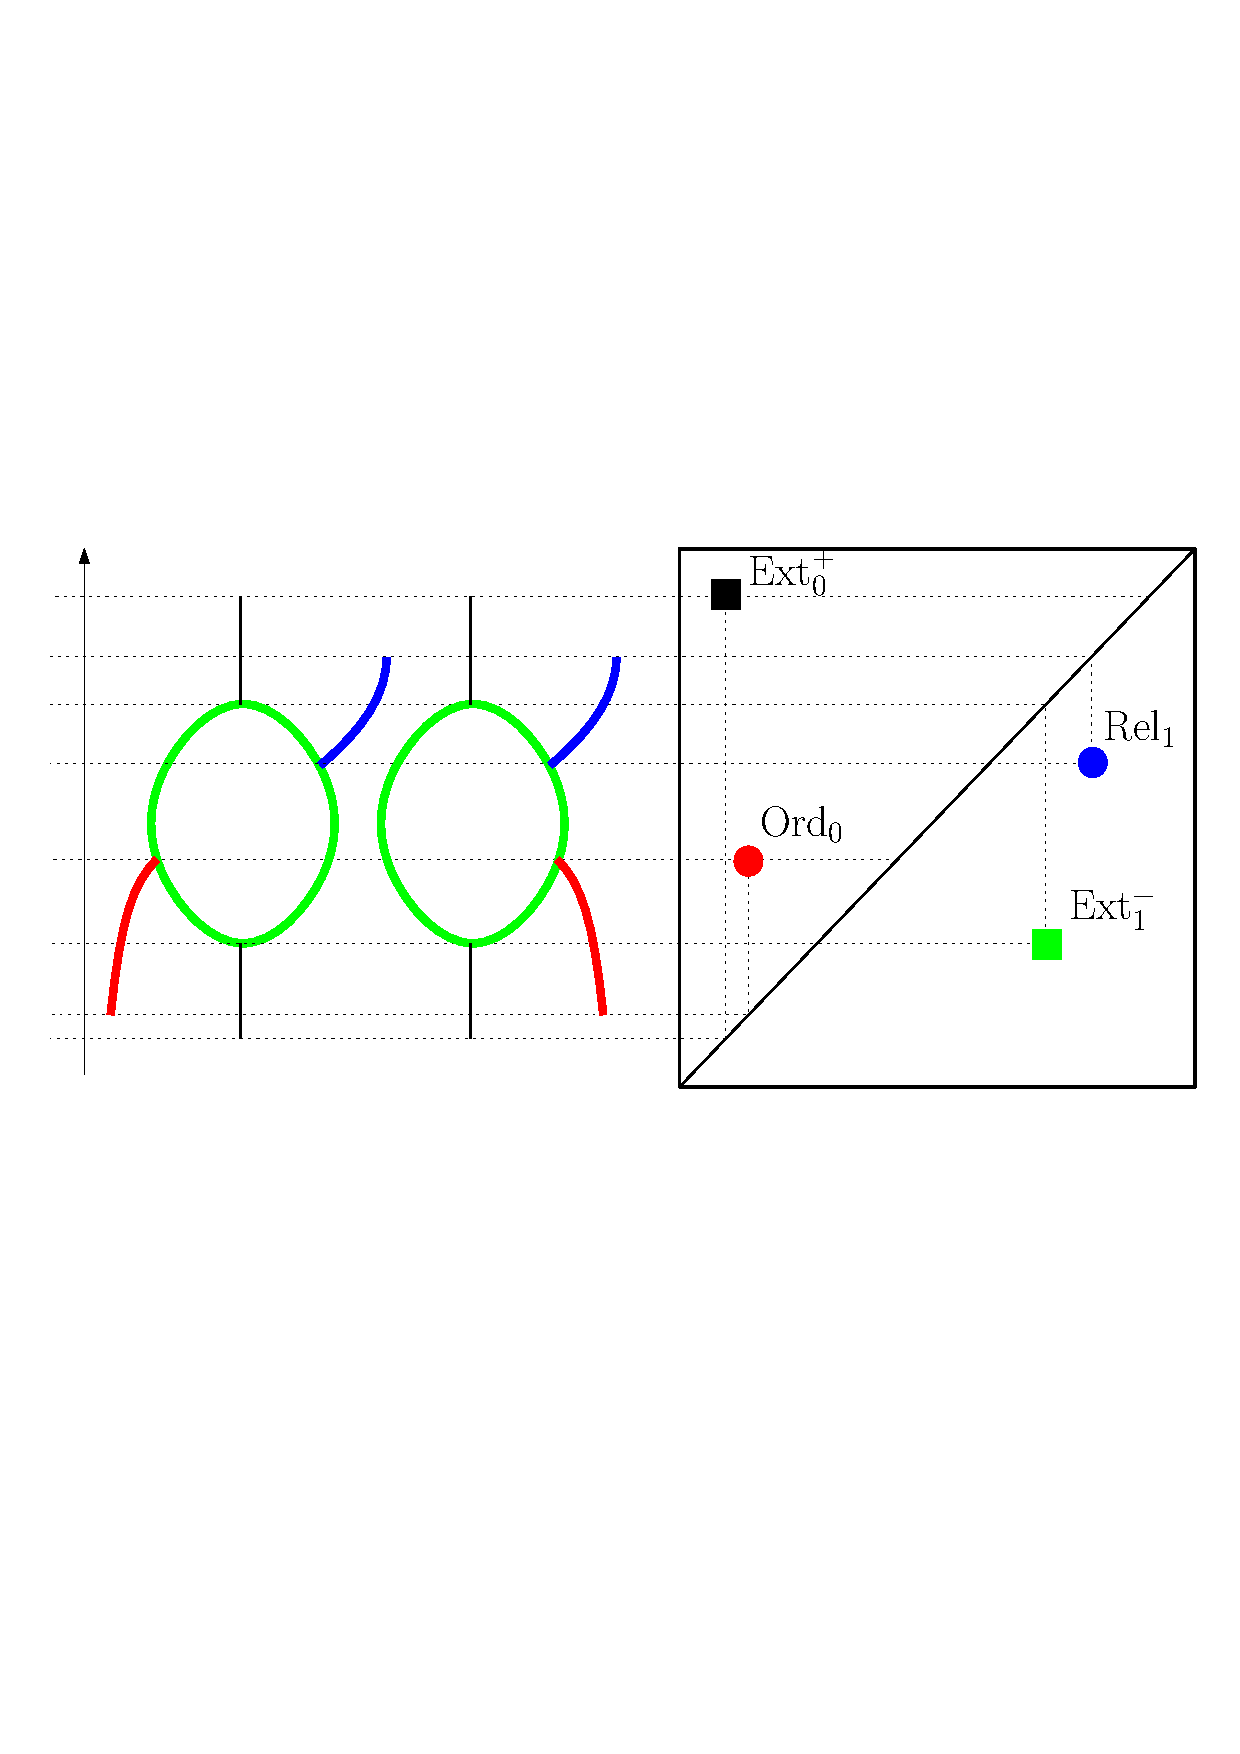
\includegraphics[width=10cm]{figures/CounterExampleMetric}
\caption{Two Reeb graphs with the same set of features but not the same layout.}
\label{fig:Reeb_struct}
\end{figure}



\subsubsection*{Connection to the extended and levelset zigzag persistence of~$f$.}
\label{sec:topologyReeb}

We now show that the topological structure of $\Reeb_f(X)$ is actually nothing but a simplification 
of the one of $f$, which we phrase in terms of persistence diagrams. 
This result and its proof can be seen as an exercise combining all concepts introduced before in a simple way.
%can be phrased using the levelset zigzag and extended persistence modules of $f$ and $\tilde f$, and

\begin{thm}\label{thm:pdreeb}
Let $X$ be a topological space and
$f:X\rightarrow\R$ be a function of Morse type.
Then, the levelset zigzag persistence barcodes of $f$ and $\tilde f$ in dimension 0 are the same: $\DgZZ_0(f)=\DgZZ_0(\tilde f)$,
and the extended persistence diagram of $\tilde f$ is included in the one of $f$: $\Dg(\tilde{f})\subseteq \Dg(f)$.
More precisely:
\begin{align*}
\Dg_0(\tilde{f}) &= \Dg_0(f) \\
\Dg_1(\tilde{f}) &= \Dg_1(f)\setminus(\Ext^+_1(f)\cup\Ord_1(f)) \\
\Dg_p(\tilde{f}) &= \emptyset\text{  if }p\geq 2
\end{align*}
\end{thm}

Note that  $\Ext_0^-(\tilde f)%= \Ext_0^-(f)
%=\Ext_0^-(\fMMtel)= \Ext_0^-(\fRMMtel)
= \emptyset$ because every
essential $0$-dimensional feature corresponds to some connected component of the
domain, and it is born at the minimum function value and killed at the
maximum function value over that connected component, hence it belongs to $\Ext_0^+$.
%Moreover, %$\Rel(\tilde f)=\Rel_1(\tilde f)$ since 
Similarly, $\Rel_0(\tilde f)=\emptyset$
because no 0-dimensional homology class (i.e. connected component) can be
created in the relative part of the extended filtration of~$f$. 
%We  also recall that $\Ext_0^-(f)$ is empty too.
Hence, the structure of a Reeb graph can be read off from the levelset zigzag persistence module of $\tilde f$.
Indeed, since $\Ext_1^+(\tilde f)$, $\Ord_1(\tilde f),\Ext_0^-(\tilde f),\Rel_0(\tilde f)$ and $\Dg_p(\tilde f)$ for $p\geq 2$ are empty, 
it follows from Corollary~\ref{cor:EPZZ} that 
there is a bijection preserving types between $\Dg_0(\tilde f)\cup\Dg_1(\tilde f)$ and $\DgZZ_0(\tilde f)$. 
This is because all intervals in the 1-dimensional extended persistence module of $\tilde f$ 
are either of type $\Rel$ or $\Ext^-$, and thus their analogues in the levelset zigzag persistence module of $\tilde f$ have 
homological dimension 0 according to Table~\ref{tab:EPZZ}.

%Hence, according to Theorem~\ref{thm:pdreeb} and Corollary~\ref{cor:EPZZ},
%there is a bijection between $\Dg_0(\tilde f)\cup \Dg_1(\tilde f)$ and $\DgZZ_0(\tilde f)$.

We now provide a proof of Theorem~\ref{thm:pdreeb} for completeness, 
as we have not seen this result  stated formally in the literature. 
First, note that $\Crit(f)=\{a_1,\cdots,a_n\}=\Crit(\tilde f)$. 
Hence, given $i\leq j$ and $[s_i,s_j]$ as in Definition~\ref{def:LZZ}, %Section~\ref{sec:ZZ},
we recall that $X_i^j$ denote $X^{[s_i,s_j]}=f^{-1}([s_i,s_j])$ and $\Reeb_f(X)_i^j$ denote $\Reeb_f(X)^{[s_i,s_j]}=\tilde f^{-1}([s_i,s_j])$.

\begin{lem}\label{lem:ZZ0}
Let $\pi$ denote the quotient map $X\rightarrow\Reeb_f(X)$.
Let $i\leq j$.
%and $I=[s_i,s_j]$, as defined in Section~\ref{sec:ZZ}.
Then the morphism $\pi_*:H_0(X_i^j)\rightarrow H_0(\Reeb_f(X)_i^j)$ 
is an isomorphism.
\end{lem}

The proof of Lemma~\ref{lem:ZZ0} is
simpler when $\pi$ admits {\em continuous sections}, i.e. when there exist
continuous maps $\sigma:\Reeb_f(X)\rightarrow X$ such that
$\pi\circ\sigma=\text{id}_{\Reeb_f(X)}$.
Below we give the proof under this hypothesis, deferring 
the general case of Morse-type functions to
Appendix~\ref{sec:proof_pdreeb}.  The hypothesis holds for instance
when $X$ is a compact smooth manifold and $f$ is a Morse function, or
when $X$ is a simplicial complex and $f$ is piecewise-linear.

\begin{proof}
Since $\pi$ is surjective, proving the result boils down to
showing that $x,y$ are connected in 
$X^j_i$ if and only if $\pi(x),\pi(y)$ are connected in $\Reeb_f(X)_i^j$.

\begin{itemize}
\item If $x,y$ are connected in $X^j_i$,
then $\pi(x),\pi(y)$ are connected in $\Reeb_f(X)^j_i$
by continuity of $\pi$ and
commutativity of~(\ref{eq:triangleReeb}).
%
\item If $\pi(x),\pi(y)$ are connected in $\Reeb_f(X)^j_i$,
then choose a path $\gamma$ connecting $\pi(x)$ to $\pi(y)$. By definition of~$\sigma$, we have
$\pi\circ\sigma\circ\pi(x)=\pi(x)$, thus $\sigma\circ\pi(x)$ and
$x$ lie in the same connected component of $f^{-1}(f(x))$.  Let $\gamma_x$ be a path
connecting $x$ to $\sigma\circ\pi(x)$. Similarly, let $\gamma_y$
be a path connecting $\sigma\circ\pi(y)$ to $y$. Then,
$\gamma_y\circ\sigma(\gamma)\circ\gamma_x$ is a path between $x$ and $y$ in $X^j_i$.
\end{itemize}

\end{proof}

\begin{proof}[Proof of Theorem~\ref{thm:pdreeb}]

We first show that $\DgZZ_0(f)=\DgZZ_0(\tilde f)$. Let $\pi$ denote the quotient map $X\rightarrow\Reeb_f(X)$.
Since $\pi$ is continuous, it induces a morphism in homology $\pi_*$. We will show that $\pi_*$ 
induces an isomorphism between $\LZZ(f)$ and $\LZZ(\tilde f)$ in dimension~0.

Now, let $1\leq i\leq n$.

\begin{itemize}
\item According to Lemma~\ref{lem:ZZ0}, $\pi_*:H_0(X_i^i)\rightarrow H_0(\Reeb_f(X)^i_i)$ is an isomorphism, and 
the same holds for $\pi_*:H_0(X_i^{i+1})\rightarrow H_0(\Reeb_f(X)^{i+1}_i)$. Hence $\pi_*$ induces a pointwise isomorphism 
in dimension~0 between $\LZZ(f)$ and $\LZZ(\tilde f)$. Since $\Crit(f)=\{a_1,\cdots,a_n\}=\Crit(\tilde f)$,
it follows that both $\LZZ(f)$ and $\LZZ(\tilde f)$ have $2n+1$ nodes.
\item Let $\iota:X^i_i\rightarrow X_i^{i+1}$ and
 $\iota^{\Reeb}:\Reeb_f(X)^{i}_i\rightarrow \Reeb_f(X)^{i+1}_i$
be canonical inclusions. Then, we have $\pi\circ\iota=\iota^{\rm R}\circ\pi$ 
by definition of $\iota^{\rm R}$.
Hence, the following diagram commutes:
$$\xymatrix@!C{
H_0(X^i_i) \ar[r]^-{\iota_*} \ar[d]_-{\pi_*} & H_0(X^{i+1}_i) \ar[d]^-{\pi_*} \\
H_0(\Reeb_f(X)^i_i) \ar[r]_-{\iota^{\Reeb}_*} & H_0(\Reeb_f(X)^{i+1}_i)
}$$
and the same is true for the canonical inclusions $X^i_{i-1}\hookleftarrow X_i^{i}$ and
 $\Reeb_f(X)^{i}_{i-1}\hookleftarrow \Reeb_f(X)^{i}_i$.
\end{itemize}

Hence, the induced pointwise isomorphism is an isomorphism between $\LZZ_0(f)$ and $\LZZ_0(\tilde f)$.

Now, recall that there is a bijection $b_1$ preserving types between $\Dg(\tilde f)$ and $\DgZZ_0(\tilde f)$.
Since there is also a bijection $b_2$ preserving types between $\DgZZ_0(\tilde f)$ and $\DgZZ_0(f)$
and a bijection $b_3$ preserving types between $\DgZZ_0(f)$ and $\Ord_0(f)\cup\Ext_0^+(f)\cup\Rel_1(f)\cup\Ext_1^-(f)$ from Corollary~\ref{cor:EPZZ},
the result follows by considering the bijection $b_3\circ b_2 \circ b_1$. 
\end{proof} 


















\subsection{Metrics between Reeb graphs}
\label{sec:metrics}

%Several stable distances have been derived to compare Reeb graphs, such as 
%the {\em edit distance $\diste$}~\cite{DiFabio16, Bauer16},
%the {\em functional distortion distance $\distfd$}~\cite{Bauer14},
%the {\em interleaving distance $\disti$}~\cite{deSilva16},
%which has been proven strongly equivalent to $\distfd$ in~\cite{Bauer15}, 
%and the {\em bottleneck distance $\distb$}, which is only a pseudo metric. 
%In this chapter, we focus on $\distfd$, which is the most natural analogue of the Gromov-Hausdorff distance
%for Reeb graphs, and $\distb$. We will show in Section~\ref{sec:lowerbound} that these distances are actually
%{\em locally} equivalent.

%\paragraph*{Metrics and pseudometrics.}
Finding relevant dissimilarity measures for comparing Reeb graphs has become an important question in the recent years.
The quality of a dissimilarity measure is usually assessed through three criteria: 
its ability to satisfy the axioms of a metric, its discriminative power, and its computational efficiency.  	
The most natural choice to begin with is to use the {\em Gromov-Hausdorff distance} $d_{\rm GH}$~\cite{Burago01} for Reeb graphs 
seen as metric spaces---see Definition~\ref{def:metricReeb}.  
The main drawback of this distance is to quickly become intractable to compute in practice, even for graphs that are metric trees~\cite{Agarwal15}.
Among recent contributions, the {\em functional distortion distance}
$\distfd$~\cite{Bauer14}, the {\em interleaving distance} $\disti$~\cite{deSilva16}---which is equivalent to $\distfd$~\cite{Bauer15}---
and the {\em edit distance $\diste$}~\cite{Bauer16,DiFabio16} share the same advantages and drawbacks as
$\distgh$, in particular they enjoy good stability and
discriminativity properties but they lack efficient algorithms for
their computation, moreover they can be difficult to interpret.  By
contrast, the {\em bottleneck distance} $\distb$
compares Reeb graphs with their extended persistence diagrams---which act as stable
bag-of-features signatures---and can be computed
efficiently in practice.  Its main drawback though is to be only a
pseudometric, so distinct graphs can have the same signature and
therefore be deemed equal in $\distb$---see Figure~\ref{fig:Reeb_struct}. We now give details on these distances.



%Reeb graphs are often used as descriptors for data, hence defining metrics to compare them is
%of particular interest. Since Reeb graphs are metric spaces, with intrinsic metrics given by Definition~\ref{def:metricReeb}, 
%the first natural distance between Reeb graphs is the {\em Gromov-Hausdorff distance}~\cite{Burago01}.	

\paragraph*{The Gromov-Hausdorff distance $\distgh$.} This distance compares Reeb graphs by computing the length distortion 
of corresponding curves drawn on the graphs.
%
\begin{defin}\label{def:dgh}
Let $X,Y$ be topological spaces and $f:X\rightarrow\R$, $g:Y\rightarrow\R$ be continuous functions.
The {\em Gromov-Hausdorff distance} between $\Reeb_f(X)$ and $\Reeb_g(Y)$ is:
\begin{equation}\label{eq:dgh}
\distgh(\Reeb_f(X),\Reeb_g(Y))=\underset{\phi,\psi}{\rm inf}\ D(\phi,\psi),
\end{equation}
where: 
\begin{itemize}
\item $\phi:\Reeb_f(X)\rightarrow\Reeb_g(Y)$ and $\psi:\Reeb_g(Y)\rightarrow\Reeb_f(X)$ are (nonnecessarily continuous) maps, 
\item $D(\phi,\psi)=\frac 12\ {\rm sup}\ \left\{|d_f(x,x')-d_g(y,y')|\,:\,(x,y),(x',y')\in C(\phi,\psi)\right\},$ %where
\item 
$C(\phi,\psi)=\{(x,\phi(x))\, :\, x\in\Reeb_f(X)\}\cup\{(\psi(y),y)\, :\, y\in\Reeb_g(Y)\}$.
\end{itemize}
\end{defin}
%
The main drawback of $\distgh$ is that it does not fully take function values into account. For instance,
it is straightforward to show that $\distgh(\Reeb_f(X),\Reeb_{-f}(X))=0$ and $\distgh(\Reeb_f(X),\Reeb_{f+c}(X))=0$,
where $c\in\R$. %is a constant. 

\paragraph*{Functional distances.}
To handle this issue, Bauer et al.~\cite{Bauer13a} suggested to add terms corresponding
to the absolute difference in function values:
%
\begin{defin}[\cite{Bauer13a}]\label{def:dfgh}
Let $X,Y$ be topological spaces and $f:X\rightarrow\R$, $g:Y\rightarrow\R$ be continuous functions.
The {\em functional Gromov-Hausdorff distance} between $\Reeb_f(X)$ and $\Reeb_g(Y)$ is:
\begin{equation}\label{eq:dfgh}
\distfgh(\Reeb_f(X),\Reeb_g(Y))=\underset{\phi,\psi}{\rm inf}\ \max\{D(\phi,\psi),\|f-g\circ\phi\|_\infty,\|f\circ\psi-g\|_\infty\},
\end{equation}
where $\phi$, $\psi$ and $D(\phi,\psi)$ are as in Definition~\ref{def:dgh}. 
\end{defin}
%
In Section~\ref{sec:lowerbound}, we will show that the functional Gromov-Hausdorff distance is actually {\em locally}
equivalent to the bottleneck distance between the extended persistence diagrams of the functions. To ease the analysis,
we will use a third distance which constrains the maps $\phi$ and $\psi$ to be continuous.
%
\begin{defin}[\cite{Bauer14}]\label{def:dfd}
Let $X,Y$ be topological spaces and $f:X\rightarrow\R$, $g:Y\rightarrow\R$ be continuous functions.
The {\em functional distortion distance} between $\Reeb_f(X)$ and $\Reeb_g(Y)$ is:
\begin{equation}\label{eq:dfd}
\distfd(\Reeb_f(X),\Reeb_g(Y))=\underset{\phi,\psi}{\rm inf}\ \max\{D(\phi,\psi),\|f-g\circ\phi\|_\infty,\|f\circ\psi-g\|_\infty\},
\end{equation}
where $\phi$, $\psi$ and $D(\phi,\psi)$ are as in Definition~\ref{def:dgh}, and where we also require
$\phi$ and $\psi$ to be continuous. 
\end{defin}
%
Requiring the maps to be continuous has very little impact on the distance properties since $\distfgh$ and $\distfd$ are {\em strongly equivalent}:
%
\begin{thm}[Theorem 5.1 in~\cite{Bauer13a}]\label{th:dfddfgheq}
Let $X,Y$ be topological spaces and $f:X\rightarrow\R$, $g:Y\rightarrow\R$ be continuous functions.
Then: $$\distfgh(\Reeb_f(X),\Reeb_g(Y))\leq\distfd(\Reeb_f(X),\Reeb_g(Y))\leq3\distfgh(\Reeb_f(X),\Reeb_g(Y)).$$
\end{thm}
%
Furthermore, these distances are stable with respect to changes in the function:
%
\begin{thm}[Theorem 4.1 in~\cite{Bauer14}]\label{th:dfdstab}
Let $X$ be a topological space and let $f,g:X\rightarrow\R$ be two Morse-type functions with continuous sections.
Then:
$$\distfgh(\Reeb_f(X),\Reeb_g(X))\leq\distfd(\Reeb_f(X),\Reeb_g(X))\leq \|f-g\|_\infty.$$
\end{thm}




\paragraph*{The bottleneck distance $\distb$.} This distance uses the extended persistence diagrams of the functions to compare the Reeb graphs.

\begin{defin}\label{def:BottleDistReeb}
Let $X,Y$ be topological spaces and $f:X\rightarrow\R$, $g:Y\rightarrow\R$ be continuous and tame functions.
The {\em bottleneck distance} between $\Reeb_f(X)$ and $\Reeb_g(Y)$ is:
\begin{equation}\label{eq:db}
\distb(\Reeb_f(X),\Reeb_g(Y))=\distb(\Dg(\tilde f), \Dg(\tilde g)),
\end{equation}
where $\tilde f:\Reeb_f(X)\rightarrow \R$ and $\tilde g:\Reeb_g(Y)\rightarrow \R$ are the induced maps on the Reeb graphs.
\end{defin}

As a direct application of the stability theorem---see Theorem~\ref{th:ExStab}, 
the bottleneck distance is also stable with respect to changes in the function.

%\paragraph*{Other distances.} Reeb graphs can also be compared with 
%the {\em interleaving distance $\disti$}~\cite{deSilva16} 
%However, since the interleaving distance has been proven equivalent to $\distfd$ and $\distfgh$ in~\cite{Bauer15} 
%and the edit distance is more suited to combinatorial graphs, we leave these distances aside. 


\paragraph*{A first inequality.} Bauer et al.~\cite{Bauer14} related $\distfd$ and $\distb$ as follows:
%
\begin{thm}[Theorem 4.3 in~\cite{Bauer14}]\label{th:weakupperbound}
Let $X,Y$ be topological spaces and $f:X\rightarrow\R$, $g:Y\rightarrow\R$ be continuous and tame functions.
The following inequality holds: 
$$\distb(\Reeb_f(X),\Reeb_g(Y))\leq 3\,\distfd(\Reeb_f(X),\Reeb_g(Y)).$$
\end{thm}
%
This result can be improved using the end of Section~3.4 of~\cite{Bjerkevik16}
(using the fact that levelset zigzag persistence barcodes and extended persistence diagrams are essentially the same---see Corollary~\ref{cor:EPZZ}), 
and then Lemma~9 of~\cite{Bauer15} and Theorem~\ref{th:dfddfgheq}:
%
\begin{thm}\label{th:upperbound}
Let $X,Y$ be topological spaces and $f:X\rightarrow\R$, $g:Y\rightarrow\R$ be continuous and tame functions.
The following inequality holds: 
$$\distb(\Reeb_f(X),\Reeb_g(Y))\leq 2\,\distfd(\Reeb_f(X),\Reeb_g(Y))\leq 6\,\distfgh(\Reeb_f(X),\Reeb_g(Y)).$$
\end{thm}
%



\subsection{Simplification techniques}\label{sec:simplopReeb}

Being able to simplify Reeb graphs by removing small topological features is very useful.
It very often helps to prove theoretical results concerning Reeb graphs, and has many applications, 
for instance in Reeb graph computation and visualization~\cite{Ge11, Pascucci07, Tierny15}. 

In this section, we define one possible way to do such a simplification, that we will 
use in Section~\ref{sec:lowerbound} of Chapter~\ref{chap:backgroundTelescopesReeb} to prove Theorem~\ref{th:locisom}. 
%More precisely, we define an operator for loops and branches of Reeb graphs.  
We recall that, due to the bag-of-feature interpretation of $\Dg(\tilde f)$, 
any point $p=(a,b)\in\Dg(\tilde f)\setminus \Ext_0^+(\tilde f)$ represents either an upward branch, 
a downward branch or a loop. 
%Moreover, the vertical span of the corresponding feature, that we denote $\gamma$, is 
%$[\min_{x\in\gamma} \tilde f(x),\ \max_{x\in\gamma} \tilde f(x)]=[a,b]$
%(we do not use infimum and supremum since $f$ is of Morse type, and thus extrema in $\gamma$ are achieved).
Depending on the feature type, we define the {\em merging path} $\pi^p$ as follows:
\begin{itemize}

\item assume $p\in\Ext_1^-(\tilde f)$, i.e. $p$ represents a loop 
with extremities $x_1,x_2\in\Reeb_f(X)$, so that we have $\tilde f(x_1)=a$ and $\tilde f(x_2)=b$.
Let $\pi_1^p$ and $\pi_2^p$ be two disjoint sub-curves of the loop that connect $x_1$ and $x_2$.
Then, we let $\pi^p=\pi_1^p\cup\pi_2^p$.

%\item assume $p\in\Ext_0^+(\tilde f)$, i.e. $p$ represents a connected component
%with extremities $x_1,x_2\in\Reeb_f(X)$, so that we have $\tilde f(x_1)=a$ and $\tilde f(x_2)=b$.
%Then, we let $\pi^p$ be an arbitrary path connecting $x_1$ and $x_2$.

\item assume $p\in\Ord_0(\tilde f)\cup \Rel_1(\tilde f)$, i.e. $p$ represents a branch.
Let $C_1$ be this branch. If $p\in\Ord_0(\tilde f)$ (resp. $\Rel_1(\tilde f)$), let $C_2$ be an arbitrary connected component of 
$\tilde f^{-1}((-\infty,b))$ (resp. $\tilde f^{-1}((b,+\infty))$)
to which $C_1$ gets connected at level $b$. We define the triple $x_1,x_2,y$ as follows:
$$
%\begin{array}{c|c|c} 
%x_1 = 
\left\{\begin{array}{l} 
x_1={\rm argmin}_{x\in C_1}\tilde f(x),y={\rm argmax}_{x\in C_1}\tilde f(x)\text{ and }x_2= {\rm argmin}_{x\in C_2}\tilde f(x)\text{ if }p\in\Ord_0(\tilde f)\text{ and } \\ 
x_1={\rm argmax}_{x\in C_1}\tilde f(x),y={\rm argmin}_{x\in C_1}\tilde f(x)\text{ and }x_2= {\rm argmax}_{x\in C_2}\tilde f(x)\text{ if }p\in\Rel_1(\tilde f).
\end{array}\right.$$ 
%y   = \left\{\begin{array}{l} {\rm argmax}_{x\in C_1} \tilde f(x)\text{ if }p\in\Ord_0(\tilde f) \\ {\rm argmin}_{x\in C_1} \tilde f(x)\text{ if }p\in\Rel_1(\tilde f)\end{array},\right. 
%x_2 = \left\{\begin{array}{l} {\rm argmin}_{x\in C_2} \tilde f(x)\text{ if }p\in\Ord_0(\tilde f) \\ {\rm argmax}_{x\in C_2} \tilde f(x)\text{ otherwise}\end{array},\right. 
%\end{array}$$
 
Note that we have $\tilde f(x_1)=a$ and $\tilde f(y)=b$ in both cases.
We now let $\pi_1^p$ be any arbitrary path from $x_1$ to $y$ and  $\pi_2^p$ be any arbitrary path from $y$ to $x_2$.
Finally, we let $\pi^p=\pi_1^p\cup\pi_2^p$ as before.

\end{itemize}

\begin{defin}[\cite{Bauer14,Ge11,Pascucci07}]
Let $X$ be a topological space and $f:X\rightarrow\R$ a Morse-type function.
Let $p\in\Dg(\tilde f)\setminus\Ext_0^+(\tilde f)$. We define the equivalence relation $\sim_p$ as follows:
$$
x\sim_p x' \Leftrightarrow x,x'\in\pi^p\text{ and }\tilde f(x)=\tilde f(x'). %\text{ if }p\in\Dg(\tilde f)\setminus\Ext_0^+(\tilde f).
%x\sim_p x' \Leftrightarrow x,x'\in\pi^p\text{ and }\tilde f(x)=\tilde f(x')\text{ if }p\in\Rel_1(\tilde f).
$$
See Figure~\ref{fig:simplificationop} for an illustration.
\end{defin}

\begin{figure}\centering
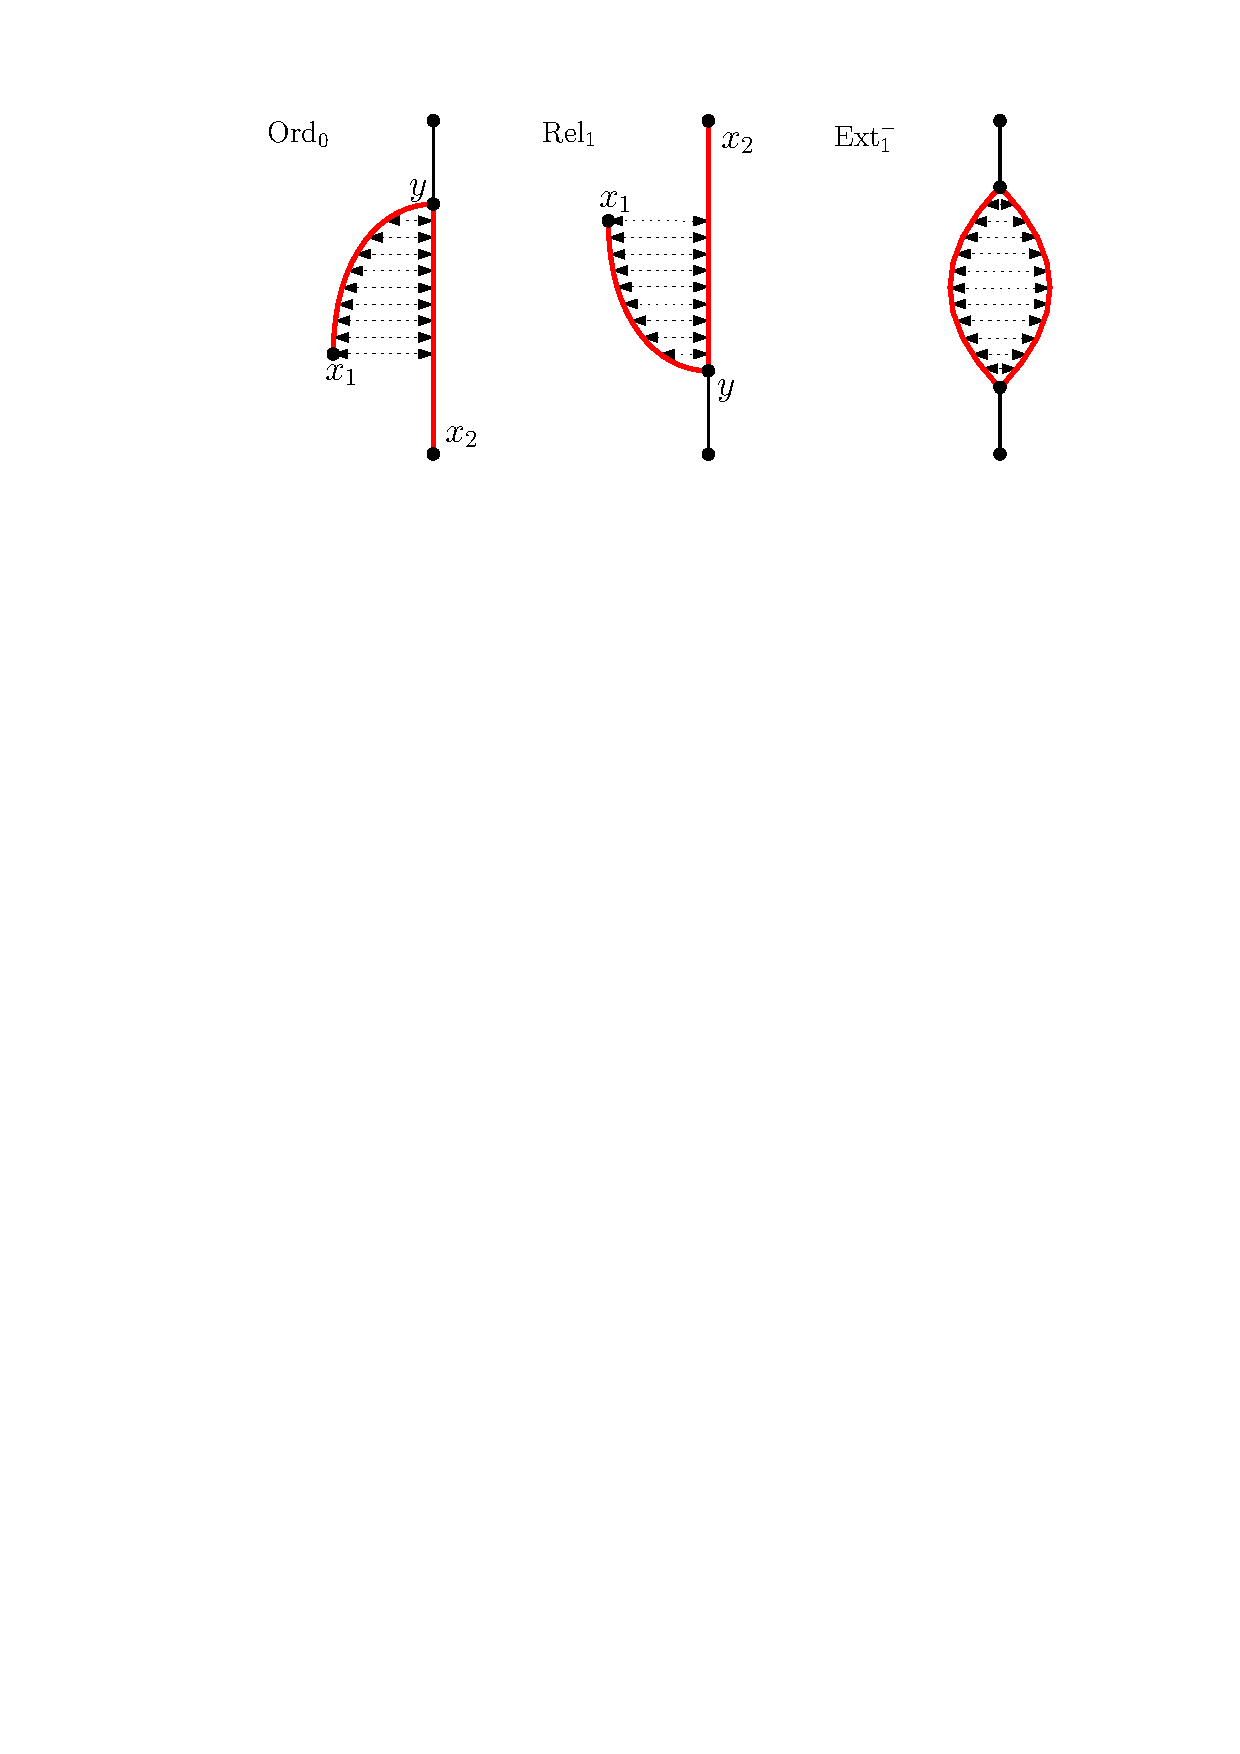
\includegraphics[height=5cm]{figures/ExampleSimplificationOp}
\caption[Feature simplification]{\label{fig:simplificationop} Dotted arrows show points that are glued together by the simplification operator depending
on the topological feature $p$, whose merging path $\pi^p$ is highlighted in red. }
\end{figure}

\begin{defin}
Let $X$ be a topological space and $f:X\rightarrow\R$ a Morse-type function.
Let $\alpha >0$, ${\rm Feat}_\alpha=\{p\in\Dg(\tilde f)\setminus \Ext_0^+(\tilde f)\,:\,2d_\infty(p,\Delta)\leq \alpha\}$
the set of points of $\Dg(\tilde f)$ representing loops and branches of $\Reeb_f(X)$ whose vertical span is less than $\alpha$
and ${\rm Conn}_\alpha$ the set of connected components of $\Reeb_f(X)$ whose vertical span is less than $\alpha$.
Finally, let $\sim_\alpha$ be the transitive closure of all $\sim_p$, where $p\in {\rm Feat}_\alpha$.
The {\em simplification operator} $S_\alpha$ is defined as:
$$S_\alpha(\Reeb_f(X))=(\Reeb_f(X)\setminus {\rm Conn}_\alpha)/\sim_\alpha.$$
\end{defin}

An illustration of the action of this operator is shown in the left part of Figure~\ref{fig:recap3}.
Intuitively, the simplification operator $S_\alpha$ removes all features  whose vertical span is less than $\alpha$
(in an arbitrary order) without perturbing the other features too much. We state this property in the following Lemma:

\begin{lem}[Theorem~7.3 and following remark in~\cite{Bauer13a}] \label{lem:stabsmooth}
Given $\alpha>0$, the simplification operator $S_\alpha$ takes any Reeb graph 
$\Reeb_h$ to $\Reeb_{h'}=S_\alpha(\Reeb_h)$ such that $\Dg(h')\cap {\rm off}_{\alpha/2}(\Delta)=\emptyset$  
and $$\distb(\Reeb_h,\Reeb_{h'})\leq 2\,\distfd(\Reeb_h,\Reeb_{h'}) \leq 4\alpha,$$
where ${\rm off}_{\alpha/2}(\Delta)=\{x\in\R^2\,:\,d_\infty(x,\Delta)\leq \alpha/2\}$ is the $(\alpha/2)$-offset
of the diagonal $\Delta$ in the $\ell_\infty$-distance.
\end{lem} 


\subsection{Computation}

One issue with the Reeb graph is the computation of the graph itself. 
Indeed, when the pair $(X,f)$ is known only through a finite set of measurements, the
graph can only be approximated within a certain error.
Building approximations from finite point samples with scalar values
is a problem in its own right. A natural approach is to build a
simplicial complex %(for instance the {\em Rips complex}) 
on top of the point samples, to serve as a proxy for the underlying continuous
space; then, to extend the scalar values at the vertices to a
piecewise-linear (PL) function over the simplicial complex by linear
interpolation; finally, to apply some exact computation algorithm for
PL functions. This is the approach advocated by Dey and
Wang~\cite{Dey13a}, who rely on the $O(n\log n)$ expected time
algorithm of Harvey, Wenger and Wang~\cite{Harvey10} for
the last step. The drawbacks of this approach are:

\begin{itemize}
\item Its relative complexity: the Reeb graph computation from the PL
  function is based on collapses of its simplicial domain that may
  break the complex structure temporarily and therefore require some repairs.
\item Its overall computational cost: here, $n$ is not the number of
  data points, but the number of vertices, edges and triangles of the
  simplicial complex, which, in principle, can be up to cubic in the number
  of data points 
  if we use a neighborhood graph. %for instance. 
  Indeed, the triangles are needed to compute an
  approximation of the Reeb graph, in the same way as they are to
  compute 1-dimensional homology.
\end{itemize}
















%%%%%%%%%%%%%%%%%%%%%%%%%%%%%%%%%%%%%%%%%%%%%%%%%%%%%%%%%%%%%%%%%%%%%%%%%%%
\section{Mapper}
\label{sec:Mapper}



%Even though Reeb graphs are powerful yet simple descriptors, they may be hard to compute, %even for metric trees~\cite{Agarwal16}.
%especially when you are given a point cloud, for which the preimages of singletons $f^{-1}(\alpha)$ are not well-defined.
To cope with the computational issue of the Reeb graph, the {\em Mapper}
was introduced by Singh, M\'emoli and Carlsson~\cite{Singh07} as a discrete version of the Reeb graph. 
%It can be seen as a generalization of the Reeb graph, since 
The main difference is that it requires to compute the connected components of preimages of {\em intervals} instead of singletons.
%This generalization is useful since the Mapper definition can be straightforwardly extended to discrete topological spaces, i.e. point clouds, 
In the case of point clouds, finding such connected components amounts to apply clustering methods on the preimages.  
%and their discrete versions, including the so-called {\em Mapper}---see Chapters~\ref{chap:MapperStability} and~\ref{chap:MapperStatistic},
%~\cite{Singh07}, 
For this reason, and due to its success in many different applications~\cite{NBA, Barra14, Lum13, Nicolau11}, 
the Mapper has become an emblematic tool of Topological Data Analysis.

It is defined in a formal way as the {\em nerve} of a specific {\em cover} of a topological space.
%The Mappers are defined with {\em nerves} of {\em covers}.
%which we detail in Section~\ref{sec:basicdef}.
%Mappers are then defined in Section~\ref{sec:Mapper}. 
%and MultiNerve Mappers are defined in Section~\ref{sec:MultiNerveMapper}.  

\subsubsection*{Covers and Nerves}
\label{sec:basicdef}

\paragraph*{Nerve of a cover.} Let $Z$ be a topological space. A {\em cover} of $Z$ is a 
family $\U$ of subsets of $Z$, $\U=\{U_\alpha\}_{\alpha\in A}$, such
that $Z=\bigcup_{\alpha\in A}\ U_\alpha$. It is {\em open} if all its
elements are open subspaces of $Z$. It is {\em connected} if all its
elements are connected subspaces of $Z$. Its {\em nerve} is the 
abstract simplicial complex $\mathcal{N}(\U)$ that has one $k$-simplex per 
$(k+1)$-fold intersection of elements of $\U$:
%
\[
\{\alpha_0,...,\alpha_k\}\in\mathcal{N}(\U)\Longleftrightarrow\bigcap_{i=0,...,k}U_{\alpha_i}\neq\emptyset.
\]

\paragraph*{Generic and minimal cover.} 
%Given a subfamily $\V$ of $\U$, we denote by $\bigcap_{\V}$ the
%intersection $\bigcap_{V\in\V}V$, and by $\bigcup_{\V}$ the union $\bigcup_{V\in\V}V$.  
When a subfamily $\V$ of $\U$ is itself a cover of $Z$, it is called
a {\em subcover} of $\U$. It is {\em proper} if it is not equal to $\U$. 
Finally, $\U$ is called {\em minimal} if it admits no proper
subcover or, equivalently, if it has no element included in the union
of the other elements.
%
Given a minimal cover $\U=\{U_\alpha\}_{\alpha\in A}$, for every
$\alpha\in A$ we let
%
\[
\tilde{U}_\alpha = U_\alpha \setminus \bigcup_{\alpha'\neq\alpha} U_{\alpha'}\cap U_\alpha,
\]
%
be the {\em proper subset} of $U_\alpha$,
that is the maximal subset of $U_\alpha$ that has an empty
intersection with the other elements of $\U$.
$\U$ is called {\em generic} if no connected component of the 
proper subsets of its elements is a singleton.






%%%%%%%%%
\subsubsection*{Mapper}
\label{sec:Mapperdef}

%%%
\begin{figure}[!t]\centering
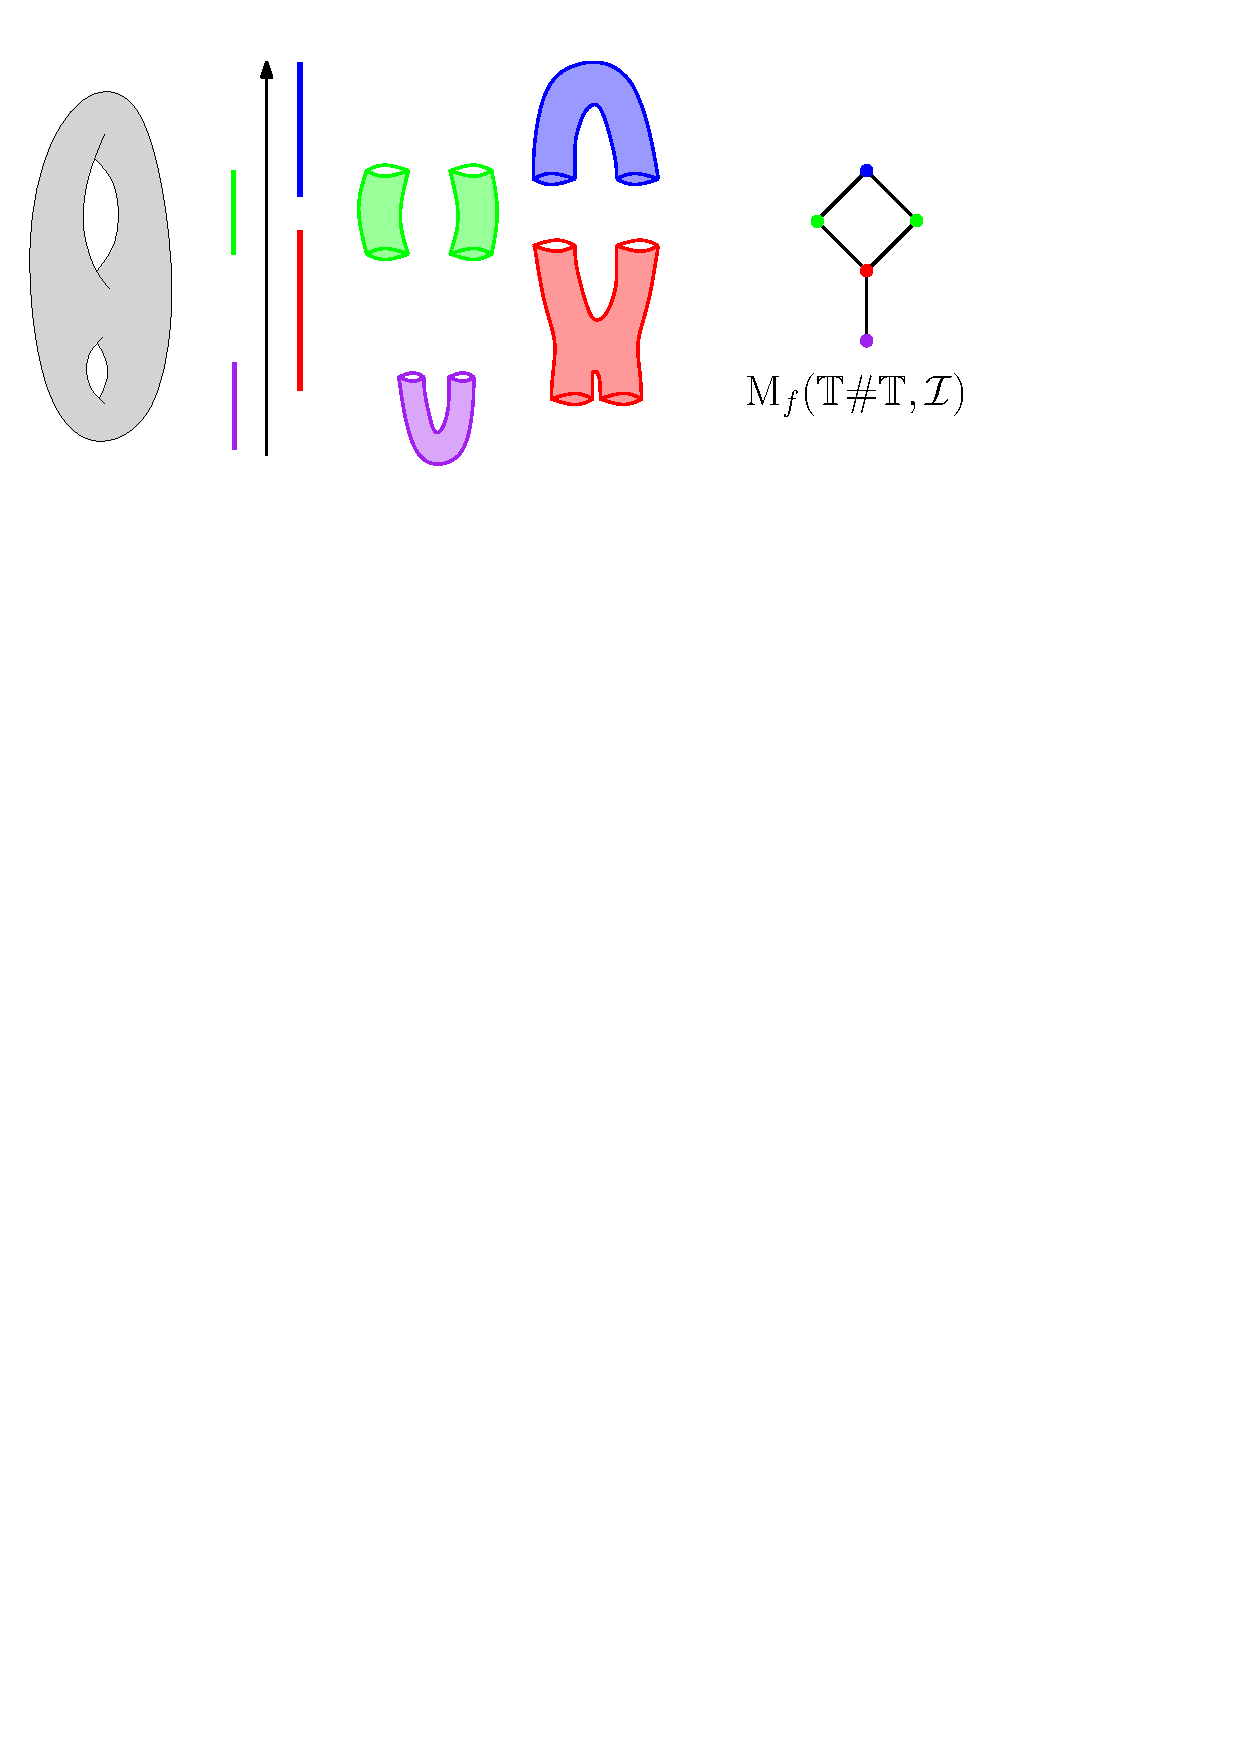
\includegraphics[height = 5cm]{figures/MMapperMapperTorus}
\caption[Mapper on double torus]{\label{fig:mmappervsmappertorus} Example of the Mapper 
%and the MultiNerve Mapper 
computed on the double torus $\mathbb T\# \mathbb T$ with the height function $f$. 
The cover $\I$ of $\im(f)\subseteq\R$ has four intervals (red, green, blue and purple), and the cover of the double torus 
has five connected components (one is blue, one is red, one is purple and the other two are green). 
The Mapper 
%and the MultiNerve Mapper are 
is displayed on the right.} 
\end{figure}

Let $X,Z$ be topological spaces and let $f:X\rightarrow Z$ be a continuous function. 
Consider a cover $\U$ of $\im(f)$, and pull
it back to $X$ via $f^{-1}$. Then, decompose every
$V_\alpha=f^{-1}(U_\alpha)\subseteq X$ into its connected components:
$V_\alpha=\bigsqcup_{i\in\{1...c(\alpha)\}}V_\alpha^i$, where
$c(\alpha)$ is the number of connected components of $V_\alpha$.  Then,
$\V=\{V_\alpha^i\}_{\alpha\in A,i\in\{1,\cdots,c(\alpha)\}}$ is a connected
cover of $X$.  It is called the {\em connected pullback cover}, and
its nerve $\Nerve(\V)$ is the Mapper.

\begin{defin}
Let $X,Z$ be topological spaces, $f:X\rightarrow Z$ be a continuous
function, $\U$ be a cover of $\im(f)$ and $\V$ be the associated
connected pullback cover.  

Then, the \emph{Mapper} of $X$ is
$\Mapper_f(X,\U)=\mathcal{N}(\V)$.
\end{defin}



See Figure~\ref{fig:mmappervsmappertorus} for an illustration.
Note that the Mapper is a simplicial complex and, as a combinatorial object, does not contain metric information. In particular,
its edges have no associated lengths.
We recall that  when the space $X$ is a point cloud, the connected pullback cover is computed with clustering. %as explained in Chapter~\ref{chap:MapperStatistic}.
We study this discrete case in more depth in Chapter~\ref{chap:MapperStatistic}, where we use single-linkage clustering. 



\subsubsection*{Computation}

The construction of Mappers from point cloud data is very easy to describe
and to implement, using standard clustering methods to detect connected
components. For instance, if single-linkage clustering is used, 
it only requires to build the edges of a single neighborhood graph, 
whose size scales up at worst quadratically (and not cubically)
with the size of the input point cloud.


%\bibliographystyle{plain}
%s\bibliography{biblio}